% **************************************************
% Document Class Definition
% **************************************************
\documentclass[%
	paper=A4,					% paper size --> A4 is default in Germany
	twoside=true,				% onesite or twoside printing
	openright,					% doublepage cleaning ends up right side
	parskip=full,				% spacing value / method for paragraphs
	chapterprefix=true,			% prefix for chapter marks
	DIV=12,
	11pt,						% font size
	headings=normal,			% size of headings
	bibliography=totoc,			% include bib in toc
	listof=totoc,				% include listof entries in toc
	titlepage=on,				% own page for each title page
	captions=tableabove,		% display table captions above the float env
	draft=false,				% value for draft version
]{scrreprt}%
\usepackage{sansmathfonts}
\usepackage{amsmath}
\usepackage{textgreek}
\usepackage{colortbl}
\usepackage{transparent}
\usepackage{eso-pic}
% for feynman diagrams
\usepackage{tikz}
\usetikzlibrary{patterns}
\usetikzlibrary{plotmarks}
\usetikzlibrary{arrows,shapes}
\usetikzlibrary{trees}
\usetikzlibrary{matrix,arrows}                 % For commutative diagram
                                            % http://www.felixl.de/commu.pdf
\usetikzlibrary{positioning}                % For "above of=" commands
\usetikzlibrary{calc,through}                % For coordinates
\usetikzlibrary{decorations.pathreplacing}  % For curly braces
% http://www.math.ucla.edu/~getreuer/tikz.html
\usepackage{pgffor}                            % For repeating patterns

\usetikzlibrary{decorations.pathmorphing}    % For Feynman Diagrams
\usetikzlibrary{decorations.markings}
\tikzset{
    >=stealth', %%  Uncomment for more conventional arrows
    vector/.style={decorate, decoration={snake}, draw},
    provector/.style={decorate, decoration={snake,amplitude=2.5pt}, draw},
    antivector/.style={decorate, decoration={snake,amplitude=-2.5pt}, draw},
    fermion/.style={draw=black, postaction={decorate},
        decoration={markings,mark=at position .55 with {\arrow{>}}}},
    fermionbar/.style={draw=black, postaction={decorate},
        decoration={markings,mark=at position .55 with {\arrow{<}}}},
    fermionnoarrow/.style={draw=black},
    gluon/.style={decorate, draw=black,
        decoration={coil,amplitude=4pt, segment length=5pt}},
    scalar/.style={dashed,draw=black, postaction={decorate},
        decoration={markings,mark=at position .55 with {\arrow{>}}}},
    scalarbar/.style={dashed,draw=black, postaction={decorate},
        decoration={markings,mark=at position .55 with {\arrow{<}}}},
    scalarnoarrow/.style={dashed,draw=black},
    electron/.style={draw=black, postaction={decorate},
        decoration={markings,mark=at position .55 with {\arrow{>}}}},
    bigvector/.style={decorate, decoration={snake,amplitude=4pt}, draw},
}

% Function to include a background picture to the titel page and following pages
\newcommand\BackgroundPic[1]{%
\centering
\begin{tikzpicture}[remember picture, overlay]
 \node[opacity=0.04,inner sep=0pt] at (current page.center)
  {\includegraphics[width=1.5\paperwidth]{#1}};
 \end{tikzpicture}
}


% **************************************************
% Debug LaTeX Information
% **************************************************
%\listfiles

% **************************************************
% Information and Commands for Reuse
% **************************************************

\newcommand{\thesisTitle}{Measurement of Higgs boson CP properties in fermionic couplings with the CMS Detector}
\newcommand{\thesisName}{Dominik Wolfschl\"ager}
\newcommand{\thesisSubject}{Masterarbeit}
\newcommand{\thesisDate}{11. Oktober 2018}
\newcommand{\thesisVersion}{Draft 1}

\newcommand{\thesisFirstReviewer}{Univ.-Prof. Dr. rer. nat. Achim Stahl}
\newcommand{\thesisFirstReviewerUniversity}{\protect{RWTH Aachen University}}
\newcommand{\thesisFirstReviewerDepartment}{}

\newcommand{\thesisSecondReviewer}{Priv.Doz. Oliver Pooth}
\newcommand{\thesisSecondReviewerUniversity}{\protect{RWTH Aachen University}}
\newcommand{\thesisSecondReviewerDepartment}{}

\newcommand{\thesisFirstSupervisor}{Prof. Dr. Achim Stahl}
\newcommand{\thesisSecondSupervisor}{}

\newcommand{\thesisUniversity}{\protect{RWTH Aachen University}}
\newcommand{\thesisUniversityDepartment}{Department of Clean Thesis Style}
\newcommand{\thesisUniversityInstitute}{Institut for Clean Thesis Dev}
\newcommand{\thesisUniversityGroup}{Clean Thesis Group (CTG)}
\newcommand{\thesisUniversityCity}{Aachen}
\newcommand{\thesisUniversityStreetAddress}{Street address}
\newcommand{\thesisUniversityPostalCode}{Postal Code}

\newcommand{\textunderscript}[1]{$_{\text{#1}}$}
% Mathe 
\makeatletter
\newcommand*{\textoverline}[1]{$\bar{\hbox{#1}}\m@th$}
\makeatother
%Nützliche Vektordefinitionen
\newcommand{\vvec}[3]{\begin{pmatrix} #1 \\ #2 \\ #3 \end{pmatrix}} %3er Spaltenvektor
\newcommand{\vecbe}[1]{\vec{\hat e}_{#1}} %EInheitsrichtungsvektor
\newcommand{\tdvec}[2]{\begin{pmatrix} #1 \\ #2 \end{pmatrix} }
\newcommand{\nullvec}{\boldsymbol{\it 0}} 
%Kugelkoordinaten
\newcommand{\ephi}{\vecbe{\phi}} %Einheitsrichtungsvektor in \phi Richtung
\newcommand{\etheta}{\vecbe{\theta}} %Einheitsrichtungsvektor in \theta Richtung

%Klammern
\newcommand{\li}{\left(} %linke Klammer (
\newcommand{\re}{\right)}%recht Klammer ) 
\newcommand{\poi}[1]{\left\{ #1 \right\}} %geschwungene Klammern { }
\newcommand{\bra}[1]{\left< #1 \right|} %angled < >
\newcommand{\ket}[1]{\left| #1 \right>}
\newcommand{\braket}[2]{ \left< #1 \right|\hspace*{-3.5pt}\left.#2 \right>} %Skalarprodukt im Hilbertraum

%Differentiale
\newcommand{\pdiff}[2]{\frac{\partial #1}{\partial #2}} %partielle Ableitung
\newcommand{\diff}[2]{\frac{\mathrm d #1}{\mathrm d #2}} %totale Ableitung
\newcommand{\pdiffc}[3]{\left( \frac{\partial #1}{\partial #2} \right)_{#3}} 

%Mathematische Symbole
\newcommand{\meq}{\overset{!}{=}}
\newcommand{\di}{\mathrm d} %aufrechtes "d" für Differentiale 
\newcommand{\origo}[1]{\mathcal O \text{(#1)}} %"Terme der Ordnung...
\newcommand{\Lagr}{\mathcal{L}} %"Terme der Ordnung...
\newcommand{\reell}{\mathbb R} %Zeichen für den reellen Zahlenraum
\newcommand{\Kern}{\mathrm{Kern} \, } 
\newcommand{\abs}[1]{\left| #1 \right| } %Betrag
\newcommand{\vecnorm}[1]{\left| \left| #1 \right| \right| } %Vektornorm
\newcommand{\matb}[1]{\mathbf #1} %Fettdruck im Mathematikmodus
\newcommand{\uuline}[1]{\underline{\underline{ #1}}} %Doppelt Underlined für Matrizen
\newcommand{\im}{\mathrm i} %für imaginäre Zahl 
\newcommand{\expe}{\mathrm e} %Eulerzahl
\newcommand{\unit}[1]{\, \text{#1} } %Aufrecht für Einheiten
\newcommand{\unitb}[1]{\, \mathbf{#1} } %Fett gedruckte Einheiten
\newcommand{\pow}[1]{\cdot 10^{#1} } 
\renewcommand{\\}{\newline \noindent} 
\newcommand{\degree}{^{\circ}}

%Sonstiges
\newcommand{\tab}{\hspace*{0.5cm}}
\newcommand{\ttab}{\hspace*{1.0cm}}
\newcommand{\cit}[1]{``#1''}
\newcommand{\Tr}{\mathrm{Tr}\ }

% particle physics
\newcommand{\htt}{$H\rightarrow\tau\tau$ }
\newcommand{\ggh}{$gg\rightarrow H$ }
\newcommand{\ttbar}{$t\bar{t}$}
\newcommand{\pt}{$p_{\text{\,T}}$}
\newcommand{\mt}{$m_{\text{T}}$}
\newcommand{\msv}{$m_{\tau\tau}$}
\newcommand{\ptautau}{$p_\text{\,T}^{\tau\tau}$}
\newcommand{\tautau}{$\tau_{\text{h}}\tau_{\text{h}}$}
\newcommand{\mutau}{$\mu\tau_{\text{h}}$}
\newcommand{\etau}{$e\tau_{\text{h}}$}
\newcommand{\emu}{$e\mu$}
\newcommand{\antikt}{\textit{anti-k\textunderscript{T}}}
\newcommand{\tauh}{$\tau_\text{h}$}
\newcommand{\jdphi}{$\Delta\phi_\text{jj}$}
\renewcommand{\eta}{\text{\textit{\texteta}}}
\renewcommand{\pi}{\text{\textit{\textpi}}}
\renewcommand{\lambda}{\text{\textit{\textlambda}}}
% **************************************************
% Load and Configure Packages
% **************************************************

\usepackage[utf8]{inputenc}		% defines file's character encoding
\usepackage[english]{babel} % babel system, adjust the language of the content
\usepackage[					% clean thesis style
	figuresep=colon,%
	sansserif=false,%
	hangfigurecaption=false,%
	hangsection=false,%
	hangsubsection=false,%
	hangsubsubsection=false,%
	colorize=full,%
	colortheme=bonbon,%
	bibsys=bibtex,%
	bibfile=bib-refs,%
	bibstyle=numeric,%
]{cleanthesis}
\usepackage{tikz-feynman}
\usepackage{subcaption}
% \usepackage{subfig}
\usepackage{tabu} 
% \pdfpageattr{/Group <</S /Transparency /I true /CS /DeviceRGB>>} 
\hypersetup{					% setup the hyperref-package options
	pdftitle={\thesisTitle},	% 	- title (PDF meta)
	pdfsubject={\thesisSubject},% 	- subject (PDF meta)
	pdfauthor={\thesisName},	% 	- author (PDF meta)
	plainpages=false,			% 	-
	colorlinks=false,			% 	- colorize links?
	pdfborder={0 0 0},			% 	-
	breaklinks=true,			% 	- allow line break inside links
	bookmarksnumbered=true,		%
	bookmarksopen=true			%
}
% \setcounter{secnumdepth}{6}
\renewcommand{\arraystretch}{1.2}
\newcommand*{\plotarchive}[1]{/Users/dominik/cernbox/www/plots_archive/#1}

\DeclareMathSizes{12}{12}{10}{9}
% **************************************************
% Document CONTENT
% **************************************************
\begin{document}
% --------------------------
% rename document parts
% --------------------------

\renewcaptionname{english}{\figurename}{Fig.}
\renewcaptionname{english}{\tablename}{Tab.}

% --------------------------
% Front matter
% --------------------------

\pagenumbering{roman}			% roman page numbing (invisible for empty page style)
\pagestyle{empty}
\newgeometry{margin=1in,bindingoffset=.5cm,showframe}				% no header or footers
% !TEX root = ../main.tex
%
% ------------------------------------  --> cover title page
\begin{titlepage}
\pdfbookmark[0]{Titlepage}{Titlepage}
% \BackgroundPic{Figures/davinci_data_analysis.jpg}
\vspace*{0.6cm}
\centering{

 { \bfseries\Huge\fontsize{34}{42}\color{ctcolormain} Search for   \\
 CP violation in fermionic couplings  \\
 of the Higgs boson  \\
 generated by gluon-gluon fusion  \\
 with the CMS Detector \\}\par

\vspace{0.5cm}

{\large von} \\ \bigskip
{\LARGE Dominik Wolfschläger}

\vspace{0.6cm}

{\Large Masterarbeit im Fach Physik} \bigskip 

{\large vorgelegt der}\\ \smallskip{}
{\Large Fakultät für Mathematik, Informatik und Naturwissenschaften der RWTH Aachen \par}

\vspace{0.3cm}

{\large im}\\ \bigskip
{\Large September 2018 } 

\vspace{0.4cm}

{\large angefertigt am}\\ \bigskip 
{\Large III. Physikalischen Institut B} 

\vspace{0.1cm}

{\large bei} \\ \bigskip
{\Large Prof. Dr. Achim Stahl}
}

\end{titlepage}
\newpage
% \BackgroundPic{Figures/davinci_overview.jpg}
\hfill
\vfill
{
\begin{minipage}{.48\textwidth}
\textbf{Erstgutachter und Betreuer}\medskip \\
Prof. Dr. Achim Stahl \\
III. Physikalisches Institut B\\
RWTH Aachen
\end{minipage}
\hfill\begin{minipage}{.32\textwidth}
{\raggedright  
\textbf{Zweitgutachter}\medskip \\
Priv. Doz. Oliver Pooth \\
III. Physikalisches Institut B\\
RWTH Aachen}
\end{minipage}
}

\restoregeometry
\cleardoublepage
%
% Table of contents
\setcounter{tocdepth}{2}		% define depth of toc
\tableofcontents				% display table of contents
\cleardoublepage


% --------------------------
% Body matter
% --------------------------

\pagenumbering{arabic}			% arabic page numbering
\setcounter{page}{1}			% set page counter
\pagestyle{maincontentstyle} 	% fancy header and footer

% INCLUDE: all titlepages
% !TEX root = ../main.tex

% standrd model is not capitalized is not a proper noun
\chapter{The Higgs boson and CP violation in the Standard Model and beyond}

The discovery of the Higgs boson in 2012 \cite{Aad:2012tfa,Chatrchyan:2012xdj} has been one of the greatest successes of the standard model (SM) of elementary particles, that is currently the most broadly accepted theory describing the fundamental constituents of matter and 
their interactions among each other. Although having defied unnumerous tests, it is insufficient because it cannot explain approved experimental observations such as the matter-antimatter asymmetry in the observable universe. 
Moreover, only three of the four known fundamental forces - the electromagnetic, strong, weak and gravitational force - can be described as a quantum theory. 
Currently, no verified quantum theory of gravitation exists and the SM and general relativity form two complementary descriptions of nature.
There are theories which solve these problems by introducing new physics that goes beyond the description of the SM. In general physicists follow two approaches to search for physics beyond the standard model (BSM). These are direct searches for  new particles and phenomena and indirect searches, where 
BSM physics leads to inconsistencies between measured SM parameters. Consequently, new physics would have been detected if any deviation from the prediction of the SM was observed in a precision measurement. 
Since the discovery of the Higgs boson, a major scientific effort has been performed to measure all the particles' properties. These include measurements of the mass $m_\text{H}$ \cite{combined_mass_Higgs}, the decay width $\Gamma_\text{H}$\,\cite{atlas_Higgswidth}, the spin and parity quantum numbers \cite{Run1_spin_parity,Run1_spinparity_ATLAS}. So far no deviation from the SM predition has been found. 
The precise determination of the properties of the Higgs boson under parity and charge-conjugation transformations, namely the CP properties, is, however, still a major challenge in Higgs physics. Being predicted as a scalar $J^\text{PC}=0^{++}$ particle, 
observations up to now only exclude the pure pseudoscalar scenario. A small pseudoscalar admixture to the prediction of the SM is still a valid scenario. The detection of such an admixture would prove CP violation in the Higgs sector, contributing potentially to the matter-antimatter asymmetry in the universe. This thesis presents a framework for an analysis that is dedicated to the precise
measurement of the CP properties of the Higgs boson in the gluon-gluon fusion process.
Beginning with a brief summary about the current understanding of elementary particles with the focus on the properties of the Higgs boson, a theoretical framework for performing a measurement of CP properties in fermionic couplings 
of the Higgs boson using an effective field theory (EFT) is motivated. In chapter \ref{chap:cms} an overview about the CMS Detector and the LHC at CERN and the reconstruction of particles from recorded signals is given.
Chapter \ref{chap:analysis} presents the setup, statistical tools, and quotes the result in terms of an expected sensitivity for the measurement of the CP mixing angle of the Higgs boson to top quarks.

\section{The Standard Model}
The SM describes the constituents of matter by \textit{elementary particles} and the fundamental \textit{electromagnetic, weak and strong forces}. 
Each particle is considered to be an excitation of a field with certain properties under symmetry transformations. Interactions between particles are based on the principle of \textit{local gauge invariance} leading to bosons that mediate these interactions. 
The SM is mathematically formulated in the framework of relativistic quantum field theories (QFT) and is expressed through a Lagrange density $\Lagr_\text{SM}$ that is invariant under local gauge transformations of the form $\text{SU(3)}_\text{C} \times \text{SU(2)}_\text{L} \times \text{U(1)}_\text{Y}$. 
The corresponding gauge bosons are 8 gluons with color charge resulting from the $\text{SU(3)}_\text{C}$, three weak bosons with weak isospin from $\text{SU(2)}_\text{L}$ and  one boson with hypercharge from $\text{U(1)}_\text{Y}$.
The importance of local gauge invariance can be inferred from t'Hooft's proof \cite{tHooft:1972tcz} that every locally gauge invariant QFT is renormizable. Renormizability enables the prevention of divergencies originating from energy ranges that lie beyond the scope of the theory by restricting the energy scale to the scale of the problem.
Feynman diagrams, which are a graphical representation of  perturbational calculus, are used to derive the matrix element that encapsulates all necessary information to calculate physics observables such as cross sections, angular distributions and decay rates.

\begin{figure}[h!]
    \centering
    \includegraphics[width=.7\textwidth]{Figures/theory/Masterthesis_diagrams_SM/Masterthesis_diagrams_SM.pdf}
    \caption[Particle content and description of the interactions of the SM.]{Particle content and description of the interactions of the SM. Fermions can be categorized into quarks and leptons. 
    According to their similar quantum numbers, but very different masses, both types of fermions are further divided into three generations that come as left-handed doublets and right-handed singlets.
    The four gauge bosons are the mediators of the strong, electromagnetic and weak interactions. By means of electroweak symmetry breaking (EWSB), the Higgs boson gives rise to the masses of the weak bosons and all fermions except for the neutrinos, that are 
    massless particles within the description of the SM and do also not form right-handed singlets. The arrows indicate that an interaction can take place between the associated bosons
     and fermions (EW: Electroweak interaction, QCD: Strong interaction). The shaded area behind some of the particle indicates that they do not couple directly to the Higgs boson and are as a consequence massless.}\label{theory:SM_infographics}
\end{figure}

\subsection{Elementary particles and interactions} 

Elementary particles are entities that do not constitute of more fundamental particles. Each particle posseses distinct quantum numbers such as mass, spin, electric charge, and color charge that precisely define its
properties and possible behaviour regarding the interaction with other particles. 
Based on the spin, it is possible to group all particles into \textit{fermions} with spin-1/2 and \textit{bosons} with integer spin.
The twelve fermions of the SM can be considered as the building blocks of matter. They come up as left-handed doublets and right-handed singlets in so-called generations with increasing mass but otherwise similar physical properties. 
\textit{Quarks} carry color charge and are the only group of elementary particles that interacts via the strong interaction, which is modeled within the theory of quantum chromodynamics (QCD). They also 
have an electric charge of $+\frac{\text{2}}{\text{3}}\text{e}$ or $-\frac{\text{1}}{\text{3}}\text{e}$ for \textit{up-type quarks} and \textit{down-type quarks}, respectively, and carry weak isospin implying that they also take part in the electroweak interaction (EW), which is the unified theory describing the electromagnetic and weak interactions. 
The remaining six fermions are called \textit{leptons}. 
The electron, muon and tau lepton have an electric charge and participate in the EW. The massless and chargeless neutrinos interact only weakly. Although it has been confirmed through the observation of neutrino-oscillations that they must possess very small masses \cite{PhysRevLett.81.1562,Ahmad:2001an,PhysRevLett.89.011301}, neutrinos are considered massless within the SM.
Bosons are force-mediators and responsible for the interaction between fermions. Thereby, the Higgs boson plays an important role as it gives mass to the fermions and EW bosons, as discussed below. \\
The sketch in \figreft{theory:SM_infographics} shows the particle content and the interactions of the SM.

\subsubsection{Quantum Chromodynamics}\label{subsec:QCD}
\begin{figure}[h!]
    \centering
    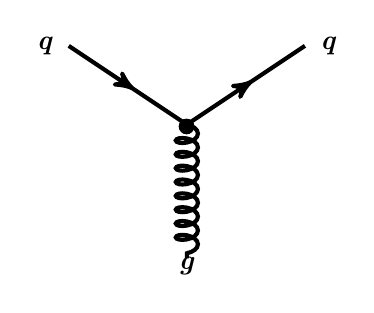
\begin{tikzpicture}[line width=1.5pt, scale=1]
% \draw[step=0.5cm, very thin, transparent] (0cm,0cm) grid (3cm,2cm);
\draw[fermion] (0cm,1.5cm) -- (1.5cm,0.5cm);
\fill[black] (0.62cm:1.57cm) circle (0.1cm);
\node at (0cm-0.3cm,1.5cm) {\textbf{\textit{q}}};
\draw[fermion] (1.5cm,0.5cm) -- (3cm,1.5cm);
\node at (3cm+0.3cm,1.5cm) {\textbf{\textit{q}}};
\draw[gluon] (1.5cm,0.5cm) -- (1.5cm, -1.2cm);
\node at (1.5cm, -1.3cm) {\textbf{\textit{g}}};
\end{tikzpicture}%
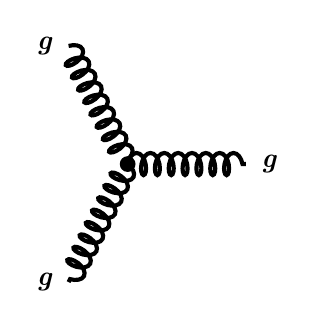
\begin{tikzpicture}[line width=1.5pt, scale=1]
% \draw[step=0.5cm, very thin, transparent] (0cm,0cm) grid (3cm,2cm);
\draw[gluon] (0cm, 1.5cm) -- (0.75cm,0cm);
\node at (-0cm-0.3cm,1.5cm) {\textbf{\textit{g}}};
\fill[black] (0:0.75cm) circle (0.1cm);
\draw[gluon] (0.75 cm,0cm) -- (0cm,-1.5cm);
\node at (0cm-0.3cm,-1.5cm) {\textbf{\textit{g}}};
\draw[gluon] (0.75cm,0cm) -- (2.25cm, 0cm);
\node at (2.25cm+0.3cm, 0cm) {\textbf{\textit{g}}};
\end{tikzpicture}%

\begin{tikzpicture}[line width=1.5pt, scale=1]
% \draw[step=0.5cm, very thin, transparent] (0cm,0cm) grid (3cm,2cm);
\draw[gluon] (0cm,1.5cm) -- (1.5cm,0cm);
\node at (0cm-0.3cm,1.5cm) {\textbf{\textit{g}}};
\draw[gluon] (1.5cm,0cm) -- (3cm,1.5cm);
\node at (3cm+0.3cm,1.5cm) {\textbf{\textit{g}}};
\draw[gluon] (1.5cm,0cm) -- (0cm, -1.5cm);
\node at (3.3cm, -1.5cm) {\textbf{\textit{g}}};
\draw[gluon] (3cm, -1.5cm) -- (1.5cm,0cm);
\node at (0cm-0.3cm, -1.5cm) {\textbf{\textit{g}}};
\fill[black] (0:1.5cm) circle (0.1cm);
\end{tikzpicture}%

    \caption[Standard vertices of QCD.]{Standard vertices of QCD. Gluon coupling to a pair of quarks (left), three gluon-vertex (middle) and 
    four-gluon vertex (right).}\label{theory:QCD_vertices}
\end{figure}

Gluons ($g$) are mediators of the strong force. There are eight gluon generators $T^a$, that are related to the $\text{3\times3}$ Gellmann-matrices $\lambda^a$  for the $\text{SU(3)}_\text{C}$ symmetry group with the relation $T^a = \frac{1}{2}\lambda^a$, corresponding 
to the eight possible non-trivial combinations and superpositions of three different colors $c$ and their associated anti-colors $\bar{c}$. 
As gluons possess an effective color charge $c\bar{c}$, too, they interact with themselves causing the possible standard vertices of QCD depicted in \figreft{theory:QCD_vertices}. The corresponding coupling structure for the QCD vertices in the Feynman diagrams is 
\begin{equation}    
    \propto g_\text{S} \frac{1}{2}\lambda^a_{ij} \gamma^\mu
\end{equation}
with a strong coupling constant $g_\text{S}$ and color factor $\lambda^a_{ij}$, that is the $ij$-th component of the Gellmann matrix of the generator $a \in \left[ 1..8\right]$. \newpage{}
$\gamma^{\mu}$ is the vector of Dirac matrices as it 
appears in the Dirac equation \cite{Thomson:2013zua}.\newline{}
The range of gluon interactions is restricted to the size of the color-neutral hadrons formed by the quarks. This \textit{color confinement} is supported by the experimental observation that
quarks and gluons do not propagate freely and hypothesizes that only particles with a net color charge equal to zero can propagate in free space. 
As a consequence, a quark or gluon being produced in a high-energy physics interaction undergoes the process of \textit{hadronization} and produces a shower of hadrons, called \textit{jet}.


\subsubsection{Quantum Flavourdynamics (QFD)}\label{subsec:QFD}
\begin{figure}[h!]
    \centering
    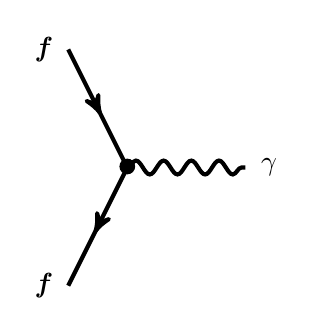
\begin{tikzpicture}[line width=1.5pt, scale=1]
% \draw[step=0.5cm, very thin, transparent] (0cm,0cm) grid (3cm,2cm);
\draw[fermion] (0cm, 1.5cm) -- (0.75cm,0cm);
\node at (-0cm-0.3cm,1.5cm) {\textbf{\textit{f}}};
\draw[fermion] (0.75 cm,0cm) -- (0cm,-1.5cm);
\node at (0cm-0.3cm,-1.5cm) {\textbf{\textit{f}}};
\draw[vector] (0.75cm,0cm) -- (2.25cm, 0cm);
\node at (2.25cm+0.3cm, 0cm) {\textbf{\textit{$\gamma$}}};
\fill[black] (1:0.75cm) circle (0.1cm);
\end{tikzpicture}%
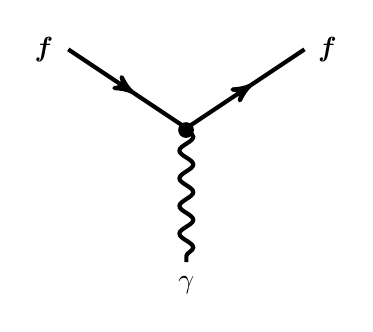
\begin{tikzpicture}[line width=1.5pt, scale=1]
% \draw[step=0.5cm, very thin, transparent] (0cm,0cm) grid (3cm,2cm);
\draw[fermion] (0cm,1.5cm) -- (1.5cm,0.5cm);
\node at (0cm-0.3cm,1.5cm) {\textbf{\textit{f}}};
\draw[fermion] (1.5cm,0.5cm) -- (3cm,1.5cm);
\node at (3cm+0.3cm,1.5cm) {\textbf{\textit{f}}};
\draw[vector] (1.5cm,0.5cm) -- (1.5cm, -1.2cm);
\node at (1.5cm, -1.5cm) {\textbf{\textit{$\gamma$}}};
\fill[black] (0.62cm:1.57cm) circle (0.1cm);
\end{tikzpicture}%
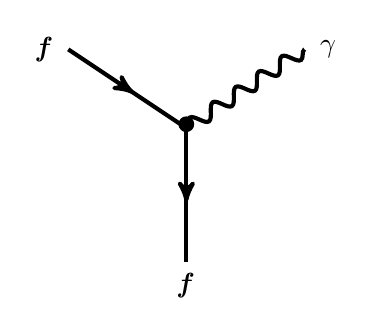
\begin{tikzpicture}[line width=1.5pt, scale=1]
% \draw[step=0.5cm, very thin, transparent] (0cm,0cm) grid (3cm,2cm);
\draw[fermion] (0cm,1.5cm) -- (1.5cm,0.5cm);
\node at (0cm-0.3cm,1.5cm) {\textbf{\textit{f}}};
\draw[vector] (1.5cm,0.5cm) -- (3cm,1.5cm);
\node at (3cm+0.3cm,1.5cm) {\textbf{\textit{$\gamma$}}};
\draw[fermion] (1.5cm,0.5cm) -- (1.5cm, -1.2cm);
\node at (1.5cm, -1.5cm) {\textbf{\textit{f}}};
\fill[black] (1.5cm,.55cm) circle (0.1cm);
\end{tikzpicture}%

    \caption[Standard vertices of QED.]{The three standard vertices of QED describe the annihilation of a fermion-antifermion pair into a photon (s-channel, left), 
    the scattering of a fermion by exchange of a photon (t-channel, middle) and the emission of a photon (right).}\label{theory:QED_vertices}
\end{figure}
The photon (\gamma) is the mediator of the electromagnetic force and couples to all particles that have an electric charge $Q$. 
Quantum electrodynamics (QED) introduces the photon field $A$ that produces the vertices indicated in \figreft{theory:QED_vertices}. The structure
for the fermion current in the Feynman diagrams at an interaction vertex of QED for fermions described by the Dirac spinor $u$ and the Dirac matrices is
\begin{equation}
    \propto Q \bar{u}\gamma^\mu u.  
\end{equation}
The $W^{\pm}$ bosons are responsible for the flavour-changing charged current (FCCC) of the weak interaction and couple to all left-handed particles possessing weak isospin $T_\text{3}$. 
The charged current produces vertices of the form
\begin{equation}
    \propto g_\text{W}\frac{1}{2}\gamma^\mu \li 1-\gamma^5\re,
\end{equation}
where $g_\text{W}$ is the weak coupling constant and $\gamma^5 = i\gamma^0\gamma^1\gamma^2\gamma^3$.\newline{}
The weak and the electromagnetic interactions
are unified within the electroweak model of Glashow, Salam and Weinberg (GSW model)\,\cite{Klapdor1989}. The neutral current (NC) induced by the Z boson is evoked by the third neutral generator $W_3^0$ of the $\text{SU(2)}_\text{L}$ gauge group to the weak isospin $T^\text{(3)}_\text{W}$ through 
mixing with a photon-like neutral field $B$ that obeyes a further $\text{U(1)}_\text{Y}$ gauge group to the weak hypercharge $Y$. Moreover, during the mixing the QED photon field $A$ is retrieved naturally. The hypercharge
is connected to both electric charge $Q$ and weak isospin $T$ by the relation
\begin{equation}
    Y = 2 \li Q - T_\text{W}^{\li 3 \re} \re. 
\end{equation}
The Feynman diagrams of the production of a W and a Z boson are shown in \figreft{theory:QFD_vertices}.
\begin{figure}[h!]
    \centering
    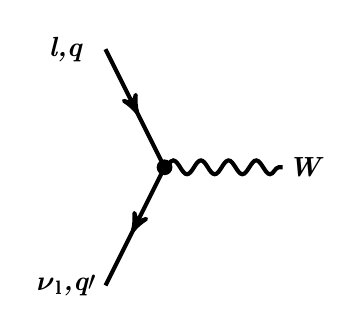
\begin{tikzpicture}[line width=1.5pt, scale=1]
% \draw[step=0.5cm, very thin, transparent] (0cm,0cm) grid (3cm,2cm);
\draw[fermion] (0cm, 1.5cm) -- (0.75cm,0cm);
\node at (-0cm-0.5cm,1.5cm) {\textbf{\textit{l,q}}};
\draw[fermion] (0.75 cm,0cm) -- (0cm,-1.5cm);
\node at (0cm-0.5cm,-1.5cm) {\textbf{\textit{$\boldsymbol{\nu}_\mathbf{l}$,q$\prime$}}};
\draw[vector] (0.75cm,0cm) -- (2.25cm, 0cm);
\node at (2.25cm+0.3cm, 0cm) {\textbf{\textit{W}}};
\fill[black] (0:.75cm) circle (0.1cm);
\end{tikzpicture}%
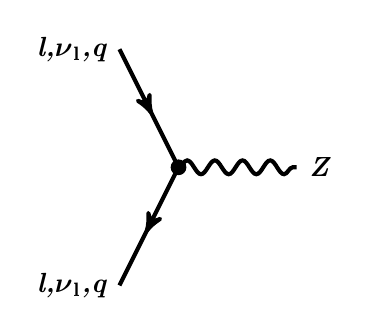
\begin{tikzpicture}[line width=1.5pt, scale=1]
% \draw[step=0.5cm, very thin, transparent] (0cm,0cm) grid (3cm,2cm);
\draw[fermion] (0cm, 1.5cm) -- (0.75cm,0cm);
\node at (-0cm-0.6cm,1.5cm) {\textbf{\textit{l,$\boldsymbol{\nu}_\mathbf{l}$,q}}};
\draw[fermion] (0.75 cm,0cm) -- (0cm,-1.5cm);
\node at (0cm-0.6cm,-1.5cm) {\textbf{\textit{l,$\boldsymbol{\nu}_\mathbf{l}$,q}}};
\draw[vector] (0.75cm,0cm) -- (2.25cm, 0cm);
\node at (2.25cm+0.3cm, 0cm) {\textbf{\textit{Z}}};
\fill[black] (0:.75cm) circle (0.1cm);
\end{tikzpicture}%

    \caption[Weak boson production Feynman graphs.]{The standard vertices of QFD describe the production of a W boson by FCCC and the production of a Z boson. There are also t-channel diagrams which are not shown here. 
            The fermions participating in the production of the W boson must possess left-handed helicity eigenvalues. }\label{theory:QFD_vertices}
\end{figure}

\subsection{The Higgs mechanism}

The Higgs mechanism is an integral part of the SM, because it ensures the self-consistency of the theory. Bosons that are introduced
through a gauge symmetry are necessarily massless particles, because mass terms of the form $m^2V^{\mu\nu}V_{\mu\nu}$ as they appear in the Klein-Gordon equation break the previously required local gauge invariance. 
Opposed to that claim, it was observed that the weak gauge bosons have very large masses, which are
responsible for the short-rangeness of the weak interaction \cite{ARNISON1983103}. The Higgs mechanism proposed independently by Brout, Englert and Higgs et al. in 1964 \cite{PhysRevLett.13.508,PhysRevLett.13.321,PhysRevLett.13.585,1964PhL....12..132H,PhysRev.145.1156} applies the 
principle of \textit{spontaneous symmetry breaking} to a scalar field with a potential of the form given in \figreft{theory:Higgs_potential}. \newline{}
\begin{figure}[!h]
    \centering
    \includegraphics[width = .5\textwidth]{Figures/theory/Higgs_potential}
    \caption[Higgs field potential.]{Projection onto the real plane of the Higgs field potential. The positions of the minima are degenerate and have a value that is different from zero. Thus, the non-zero vacuum expectation value $\nu = \text{246\,{GeV}}$ breaks 
    the symmetry of the Higgs field .}\label{theory:Higgs_potential}
\end{figure}%
In the SM two complex scalar fields are placed within a doublet of the weak isospin
\begin{equation}
    \phi = \tdvec{\phi^+}{\phi^0}. 
\end{equation}
This gives rise to four degrees of freedom that create the masses of the two W bosons and the Z boson through interaction with the scalar field. The fourth degree belongs to the 
massive boson corresponding to the scalar field. This boson is called \textit{Higgs boson}. 
Without loss of generality the scalar field can be chosen to be a real constant by gauge fixing. In the unitary gauge the ground state is
\begin{equation}
    \bra{0}\phi\ket{0} = \tdvec{0}{\nu} 
\end{equation}
with a real, positive constant $\nu$.
The Higgs mechanism creates terms of the form 
\begin{equation}
    \frac{1}{8}\nu^2 g_\text{W}^2 \li W^{\li 1 \re}_\mu W^{\li 1 \re, \mu} + W^{\li 2 \re, \mu} W^{\li 2 \re}_\mu \re + \frac{1}{8} \nu^2 \li g_\text{W} W^{\li 3 \re\,  \mu} - g^\prime B^\mu \re \li g_\text{W} W^{\li 3 \re}_\mu - g^\prime B_\mu \re 
\end{equation}
in the Lagrangian. They have the form of mass terms, and therefore the masses of the weak gauge bosons can be read off or rather be derived within the GSW model to be
\begin{equation}
    m_\text{W} = \frac{1}{2}g_\text{W}\nu \tab \text{and} \tab  m_\text{Z} = \frac{1}{2}\nu \sqrt{g_\text{W}^2 +g^{\prime2}}.
\end{equation}   
This implies that by measuring the masses and coupling constants of the W bosons and the Z boson $m_\text{W/Z}$ and $g_\text{W}/g^\prime$ the vacuum expectation value can be calculated
\begin{equation} 
    \nu = \text{246\,{GeV}}.
\end{equation} 

\subsubsection{Higgs boson Yukawa couplings}
The SM Higgs mechanism generates the masses of the W and Z bosons and solves the mass term problem for them. The 
different behaviour of left-handed and right-handed fermions, $\bar{f}_\text{L}$ and $f_\text{R}$,  under $\text{SU(2)}_\text{L}$ transformation produces Dirac mass terms of the form 
form
\begin{equation}
    \Lagr_\text{f} = -m\bar{f}f  = -m \li \bar{f}_\text{L}f_\text{R} + \bar{f}_\text{R}f_\text{L}\re
\end{equation} 
that break the gauge symmetry again.
Nevertheless, it can be shown that terms of the form 
\begin{equation}
    -y_\text{f} \left[ \bar{L}\phi R + \bar{R}\phi^\dagger L \right]
\end{equation}
and equivalent terms with the complex conjugate Higgs doublet
\begin{equation}
     \phi_\text{C} = \tdvec{-\nu-H}{0}
\end{equation}
of the form
\begin{equation}
    -y_\text{f} \left[ \bar{L}\phi_\text{C} R + \bar{R}\phi_\text{C}^\dagger L \right]
\end{equation}
 are invariant under transformations of the complete $\text{SU(2)}_\text{L} \times \text{U(1)}_\text{Y}$ symmetry group. 
Thereby, $L$ and $R$ denote the left-handed fermion doublet and right-handed fermion singlet, respectively.
For this reason, it is possible to retrieve expressions that have the form of Dirac mass terms 
\begin{equation}
    \Lagr_{\text{mass}} \propto -y_\text{f} \nu \li \bar{f}_\text{L} f_\text{R} + \bar{f}_\text{R} f_\text{L} \re = -y_\text{f} \nu  \bar{f}f.
\end{equation} 
The Yukawa coupling constants $y_\text{f}$, that were introduced above, are not predicted by the SM Higgs mechanism and must be measured. 
This means, $y_\text{f}$ is proportional to the fermion mass by construction
\begin{equation}
    y_\text{f} = \frac{m_\text{f}}{\nu}.
\end{equation}
Moreover, interaction terms between the fermions and the Higgs boson appear that are proportional to the Yukawa couplings
\begin{equation}
    \Lagr_\text{Y} \propto  -y_\text{f} H \li \bar{f}_\text{L} f_\text{R} + \bar{f}_\text{R} f_\text{L} \re = -y_\text{f} \bar{f}fH.
\end{equation} 

\subsubsection{Properties of the Higgs boson}

% describe the production and the decay
% show the relevant Feynman graphs
% pinn down the necessary cross sections
%
Given the mass of the Higgs boson of $\text{125.18\,GeV}$ \cite{Patrignani:2016xqp} the coupling strengths to other particles are fixed within the SM and production cross sections in proton-proton collisions and branching ratios can be predicted.
The two most important production processes are shown in \figreft{theory:feynman_production}.\newline{}
\begin{figure}[h!]
    \centering
    \begin{subfigure}{.49\textwidth}
        \centering
        \begin{tikzpicture}[line width=1.5pt, scale=1.2]
% \draw[step=0.5cm, very thin, transparent] (0cm,0cm) grid (4cm,2cm);

\draw[gluon] (0cm,1.25cm) -- (1.25cm,1.25cm);
\node at (0cm-0.3cm,1.25cm) {$g$};

\draw[gluon] (0cm,-1.25cm) -- (1.25cm,-1.25cm);
\node at (0cm-0.3cm,-1.25cm) {$g$};

\draw[fermion] (1.25cm,1.25cm) -- (1.25cm,-1.25cm);
\draw[fermion] (1.25cm,1.25cm) -- (2.25cm,0cm);
\draw[fermion] (2.25cm,0cm) -- (1.25cm,-1.25cm);
\node at (1.25cm-0.3cm,0cm) {$t$};
\node at (2cm-0.3cm,1.2cm) {$t$};
\node at (2cm-0.3cm,-0.2cm) {$\bar{t}$};
\draw[scalar, ctcoloraccessory] (2.25cm,0cm) -- (3.5cm,0cm);
\node at (3cm-0.3cm,-.3cm) {$H$};
\fill[black] (1.25cm,1.3cm) circle (0.1cm);
\fill[black] (0:2.25cm) circle (0.1cm);
\fill[black] (1.25cm,-1.3cm) circle (0.1cm);
\end{tikzpicture}
 
        \caption{\,Higgs boson produced via ggF.}\label{theory:feynman_production:ggF}
    \end{subfigure}
    \begin{subfigure}{.49\textwidth}
        \centering
        \begin{tikzpicture}[line width=1.5pt, scale=1]
% \draw[step=0.5cm, very thin, transparent] (0cm,0cm) grid (4cm,2cm);

\draw[fermion] (0cm,1.25cm) -- (1.25cm,1.25cm);
\node at (0cm-0.3cm,1.25cm) {$q$};
\draw[fermion] (1.25cm,1.25cm) -- (3cm,1.5cm);
\node at (3cm+0.3cm,1.5cm) {$q$};

\draw[fermion] (0cm,-1.25cm) -- (1.25cm,-1.25cm);
\node at (0cm-0.3cm,-1.25cm) {$q'$};
\draw[fermion] (1.25cm,-1.25cm) -- (3cm,-1.5cm);
\node at (3cm+0.3cm,-1.5cm) {$q'$};

\draw[vector] (1.25cm,1.25cm) -- (1.5cm,0cm);
\draw[vector] (1.25cm,-1.25cm) -- (1.5cm,0cm);

\draw[scalar, ctcoloraccessory] (1.5cm,0cm) -- (3cm,0cm);
\node at (2.5cm-0.3cm,-.3cm) {$H$};

\node at (1.5cm+0.3cm,.75cm) {$V$};
\node at (1.5cm+0.3cm,-.75cm) {$V$};
\fill[black] (1.25cm,1.25cm) circle (0.1cm);
\fill[black] (1.25cm,-1.25cm) circle (0.1cm);
\fill[black] (0:1.5cm) circle (0.1cm);
\end{tikzpicture}
 
        \caption{\,Higgs boson produced via VBF.}\label{theory:feynman_production:VBF}
\end{subfigure}
    \caption[Higgs boson production processes.]{Feynman graphs of the two most efficient production processes of the Higgs boson.}\label{theory:feynman_production}
\end{figure}
At the LHC \textref{sec:LHC} the most efficient production mechanism is the gluon-gluon fusion process (\textit{ggF}) \fref{theory:feynman_production:ggF}. The LHC is a proton collider which means the energy of the actual collision
is determined by the amount of momentum that the two colliding partons (gluon or quark) carry inside the proton. The momentum is a fraction $x$ of the total proton momentum $p_{\,\text{P}}$ and defined by the parton density functions that depict the probability that a parton carries a 
momentum fraction $x$ \cite{PhysRev.179.1547}. At the LHC energies the parton density function for gluons peaks at low values of $x$. These $x$ values are matching to the production of a Higgs boson at 125\,GeV mass.
Together with the Higgs coupling to the top quark which is in the order $\origo{1}$, this leads to the relatively high cross section of $\mathsf{\sigma_{gg\rightarrow H}} = \text{43.92\,pb}$ \cite{Heinemeyer:2013tqa}
for the ggF production process. Later in this thesis, ggF events with two initial-state jets are selected to study the CP properties of the Higgs boson \figref{theory:ggH2j_feynman}. 
These events are a next-to-next-to-leading-order (NNLO) QCD contributions and result, thus, in a cross section that is suppressed by a factor of $g_\text{s}^2$. Nevertheless, the NNLO ggF process contributes with a cross section of $\mathsf{\sigma_{gg\rightarrow Hjj}} = \text{3.98\,{pb}}$, which is still a bit larger than
the contribution from vector boson fusion (VBF)  with a cross section of $\mathsf{\sigma_{VV\rightarrow H}} = \text{3.748\,pb}$. As VBF is characterized by two forward jets originating from the remnants of the two quarks that radiate off the
vector bosons producing the Higgs boson, the topology of VBF is very similar to that of ggF events in association with two jets.

The Higgs production is decoupled from the decay because no spin information is transferred through a scalar or pseudoscalar resonance. For this reason, Higgs boson production processes can be studied with any possible decay mode. The branching ratios 
of the most frequent decay modes are given in \tabreft{theory:higgs:decay}. 

The decay into a pair of tau leptons $H\rightarrow \tau^+\tau^-$ is used to identify Higgs bosons in this thesis as this analysis built upon the SM search for the Higgs boson decaying into tau leptons \cite{Sirunyan:2017khh}. This provides on the 
one hand a relatively high yield of Higgs bosons \tabref{theory:higgs:decay} and on the other hand a settled framework for the selection of Higgs bosons. 
In the following the $H\rightarrow \tau^+\tau^-$ decay is abbreviated by $H\rightarrow \tau\tau$ keeping in mind that the tau leptons in the final state have electric charges. 

\begin{table}[!]
    \centering
    \caption[Higgs boson decay mode branching ratios.]{Decay modes and branching ratios (BR) of the SM Higgs boson \cite{Patrignani:2016xqp}.}\label{theory:higgs:decay}
    \begin{tabular}{lll}
    \toprule
    Decay mode                  & BR / \% & Remark                                                                                \\ \hline
    $H\rightarrow b\bar{b}$     & 57.8                    & Highest branching fraction, but large QCD background \cite{hbb}.                                  \\
    $H\rightarrow WW^*$         & 21.6                    & Off-shell produced W-boson \cite{ATLAS:2014aga}.                     \\
    $H\rightarrow gg$           & 8.6                     & Not detectable at LHC.                                                                \\
    \multirow{2}{*}{$H\rightarrow \tau^+\tau^-$ } & \multirow{2}{*}{6.4}                     & Largest direct coupling to leptons. \\
                            &                                         & Relatively low background compared to $b\bar{b}$ \cite{Sirunyan:2017khh}. \\
    $H\rightarrow c\bar{c}$     & 2.9                     & Not discovered yet, very large QCD backgrounds.                                        \\
    \multirow{2}{*}{$H\rightarrow ZZ^*$  }       & \multirow{2}{*}{2.7}                     & Utilized for Higgs boson discovery.                                           \\
                                            &                         & Very low background in $ZZ\rightarrow 4l$ \cite{Aad:2012tfa,Chatrchyan:2012xdj}.   \\
    \multirow{2}{*}{$H\rightarrow \gamma\gamma$} & \multirow{2}{*}{0.2}                     & Utilized for Higgs boson discovery.  \\
                                            &                         & Clear signature and low backgrounds \cite{Aad:2012tfa,Chatrchyan:2012xdj}.    \\  \bottomrule                                                  
    \end{tabular}
\end{table}

\section{CP violation}
Investigating the behaviour of physics processes under symmetry transformations can provide fundamental information about the nature of the interaction.
For example, physical processes are studied regarding the situation that 
\begin{ct_version_list}
    \item the direction of time is inverted or
    \item the coordinate system is spatially inverted.
\end{ct_version_list}
Invariance under these transformations gives fundamental insight into the physics of the process, because according to 
Emmy Noethers' theorem any symmetry leads to a conserved quantity \cite{zbMATH02611626,zbMATH02611883}.
This section gives an overview about how elementary particle interactions behave under 
parity, charge-conjugation and time-reversel transformations and the implications of violations from these laws.
\newpage{}
\subsection{Symmetry transformations}
The SM is based on the CPT-theorem, that implies that every QFT is invariant under the combination of 
\begin{ct_version_list}
    \item parity transformation $\mathcal{P}$, that inverts the coordinate system with the transformation $\vec{r}\rightarrow -\vec{r}$,
    \item charge-conjugation $\mathcal{C}$, that inverts the sign of every additive quantum number of the particle, thus turning a particle into an anti-particle and vice-versa, and 
    \item time-reversel $\mathcal{T}$, that inverts the sign of the time component $t\rightarrow -t$ and consequently changes the direction of time \cite{CPT_lueders,Pauli1988}. 
\end{ct_version_list}
The interaction terms appearing in the Lagrangian are lorentz-invariant bilinear forms that provide a distinct behaviour under these transformations. An overview about 
the different structures and their properties is given in \tabreft{theory:bilinears}.

\begin{table}[h]
    \centering
    \caption[Bilinear transformation properties.]{Behaviour of bilinear forms under $\mathcal{P}$, $\mathcal{C}$ and $\mathcal{T}$  transformations. The proofs are summarized in Ref. \cite{Nason11}. Here, $\li -1 \re^\mu$ denotes that the transformation is $+1$ if $\mu=0$ and $-1$ for $\mu \in \left[ 1,2,3\right]$, where $\mu$ is the 
     $\mu$-th component of the four-vector.}\label{theory:bilinears}
    \begin{tabular}{lcccc}
        \toprule
        Type         & Form                                 & $\mathcal{P}$               & $\mathcal{C}$ & $\mathcal{T}$                \\ \midrule
        Scalar       & $\bar{\psi}\phi$                     & $+1$                   & $+1$     & $+1$                   \\
        Pseudoscalar & $\bar{\psi}\gamma^5\phi$             & $-1$                   & $+1$     & $-1$                   \\
        Vector       & $\bar{\psi}\gamma^\mu \phi$          & $\li -1 \re^{\mu}$    & $-1$     & $\li -1 \re^{\mu}$ \\
        Axial vector & $\bar{\psi}\gamma^\mu \gamma^5 \phi$ & $-\li -1 \re^{\mu}$     & $+1$     & $\li -1 \re^{\mu}$ \\
        Tensor       & $\bar{\psi}\sigma^{\mu\nu} \phi$     & $\li -1 \re^{\mu}\li -1 \re^{\nu}$   & $-1$     &  $ -\li -1 \re^{\mu}\li -1 \re^{\nu}$ \\ \bottomrule
    \end{tabular}
\end{table}

From \tabreft{theory:bilinears} it can be inferred that 
\begin{ct_version_list}
    \item QED and QCD are invariant under CP-transformations because their fermion currents are vector couplings as given in sections \ref{subsec:QCD} and \ref{subsec:QFD}.
    \item The charged current interaction maximally violates both parity and charge-conjugation transformations individually as experimentally proven by \cite{PhysRev.105.1413}. Mathematically, the coupling structure of the weak interaction of the form $\bar{f}\gamma^\mu-\gamma^\mu \gamma^5 f$ explains this.
            The consequence of this violation is that there are no couplings to right-handed neutrinos and left-handed anti-neutrinos in the SM \cite{PhysRev.109.1015}.
\end{ct_version_list}    

Any quantum state that is eigenstate of the corresponding transformation has the eigenvalue $\pm 1$. For the CP transformation this implies, for instance,
\begin{equation}
    \mathcal{CP}\ket{\psi^{\pm}_\text{CP}} = \pm \ket{\psi^{\pm}_\text{CP}},
\end{equation} 
where +1 and -1 are the eigenvalues of the CP-even and CP-odd eigenstates, respectively. Any superposition of CP-even and CP-odd states is no longer an eigenstate of the CP transformation (see eq. \eqref{eq:CP}). Thus, CP violation is observed:
\begin{equation}\label{eq:CP}
    \mathcal{CP}\ket{\psi_\text{CP}} = \mathcal{CP}\li a \cdot \ket{\psi^{+}_\text{CP}} + b \ket{\psi^{-}_\text{CP}}  \re =  a \cdot \ket{\psi^{+}_\text{CP}} -  b \ket{\psi^{-}_\text{CP}} \neq \pm \ket{\psi_\text{CP}}.
\end{equation} 

\subsection{CP violation in the Standard Model}

Summarizing the properties of the weak interaction under C and P transformations above, one would expect that the weak interaction 
is at least invariant under simultaneous C and P transformations. In contrast to that, evidence for CP violation was reported in 
neutral Kaon decays and mixing  \cite{Christenson:1964fg,Bluemer:503743,Gorini:884851} and in B meson systems \cite{PhysRevLett.87.091801,Aubert:2002ya,PhysRevD.68.051101,PhysRevLett.91.201802,PhysRevLett.89.281802}.
Recently, the T2K experiment reported indications that CP conservation is also not conform with the neutrino sector \cite{Abe:2017uxa} pointing towards CP violation also there. CP violation in the SM has its source in the complex phase of the 3x3 CKM-matrix which relates the mass eigenstates of the quarks to their
weak eigenstates that couple to the weak gauge bosons \cite{PhysRev.105.1413}. 
CP violation occurs because this complex phase is irreducible and appears, thus, in the matrix elements for box diagrams in mixing processes, for example. 
For a brief overview about the occurence of CP violation in the SM the reader is pointed to Ref. \cite{Thomson:2013zua}. A complete and detailed theoretical description, even beyond the SM, is given in Ref. \cite{Branco:1999fs}.

\subsubsection{CP violation and the early universe}

According to the big bang theory, matter and antimatter must have been produced in equal amounts initially. 
This implies that all matter should have been annihilated into gamma rays when the density, and consequently the interaction rate, was still high enough 
in the early universe. Obviously some matter survived the annihilation phase, leading to the formation of stars and galaxies. Measurements
strongly indicate that no major abundances of antimatter are present in the observable universe today. Quantitatively, this can be 
inferred from the matter-antimatter asymmetry $\eta_\text{Asymmetry}$ that is defined by the difference of baryon $n_\text{B}$ and antibaryon $n_{\bar{\text{B}}}$ densities in relation to the cosmic microwave background photon density
\begin{equation}
    \eta_\text{Asymmetry} = \frac{n_\text{B} - n_{\bar{\text{B}}}}{n_{\gamma}} \sim 10^{-9}.
\end{equation}
In principle, the SM provides the theoretical framework required by the Sakharov conditions\,\cite{Sakharov:1967dj} that describe a physical configuration leading to a 
matter-antimatter asymmetry:
\begin{ct_version_list}
    \item Baryon number violation,
    \item CP violation and
    \item a deviation from thermal equilibrium.
\end{ct_version_list}
An estimate for the total amount of CP violation in the SM can be derived using the Jarlskog determinant $\mathcal{J}$ as defined in Ref. \cite{PhysRevLett.55.1039}. 
A dimensionless quantity can be constructed by dividing  the temperature present at the condensation of the Higgs field, when the masses of the quarks were generated, at a temperature $T_\text{EWSB}=\text{125\,{GeV}}$
\begin{equation}
    A_\text{CP} = \frac{\mathcal{J}}{T_\text{EWSB}^{12}} \approx 10^{-19} << \eta \sim 10^{-9}.
\end{equation}
\newpage{}
Comparing this roughly estimated value to the observed baryon asymmetry, it can be seen that the CP nonconservation in the SM is not large enough to explain the Baryogenesis. Therefore, the search for potentially larger sources of CP violation beyond the SM is strongly encouraged.

\subsection{Effective field Lagrangian}

In this analysis an approach utilizing an effective field theory (EFT) is followed. Thereby, the SM Lagrangian $\Lagr_\text{SM}$ 
is modified with kinematically possible new terms. Often processes are introduced at a cut-off scale $\Lambda$. Models relevant for studies aiming to determine the 
spin and parity ($J^\text{PC}$) properties of the Higgs boson are constructed by taking the SM Lagrangian, excluding the Higgs boson, and adding new terms associated with a boson $H$ with model-specific $J^\text{PC}$ properties. 
An EFT provides some advantages compared to other types of BSM theory types, that are, for instance, that
\begin{ct_version_list}
    \item only a limited set of new parameters and combinations of parameters needs to be introduced and studied,
    \item the SM is naturally recovered at low energies,
    \item every EFT is fully renormizable since orders of $\sqrt{s}/\Lambda$ in the expansion become small,
    \item if necessary, the model may be extended by adding  higher order effects or by introducing further interactions and particles.
\end{ct_version_list}
As described in Ref. \cite{Artoisenet2013} such a Lagrangian for a 
spin-0 boson has the form
\begin{equation}
    \Lagr_{\text{eff}} = \Lagr_{\text{SM Higgs}} + \Lagr_{H\text{(J=0)}}. 
\end{equation}%
For the analysis in this thesis a Lagrangian $\Lagr_{H\text{(J=0)}}$ is used that 
\begin{ct_version_list}
    \item allows for a mixing between scalar and pseudoscalar couplings of the boson,
    \item is limited to three-point interactiosn between $H$, fermions and vector bosons, meaning that only \textit{Hff} and \textit{HVV} vertices are considered, and
    \item assumes that the resonance at 125\,{GeV} belongs to a single boson. 
\end{ct_version_list} 

\subsubsection{Determining the Higgs Yukawa coupling to the top quark}
The CP properties of the Higgs boson can be fully deduced from its couplings in the production and its decay because it is a scalar or a pseudoscalar particle. There are studies dedicated 
to the measurement of the CP properties in couplings to vector bosons \cite{CMS-AN-17-034} and to tau leptons in the tau
decay channel \cite{claudia_thesis}. This analysis is dedicated to measure the CP properties in fermionic couplings in the production process which means that 
the Yukawa coupling to quarks needs to be investigated. 
At the LHC Higgs bosons are predominantly produced via ggF. As gluons are massless particles they do not couple directly to the Higgs boson. An intermediate quark loop 
is needed, and thus the effective coupling to gluons in the ggF process is studied to examine the Yukawa couplings of the Higgs boson. 
In principle, any quark flavour can run in the loop between the gluons and the Higgs boson but due to the large coupling of the top quark to the Higgs boson it becomes the 
dominant contribution. In Ref. \cite{DelDuca:2001eu} it was shown that the heavy-top quark limit $m_\text{t}\rightarrow \infty$, where the top quark is much heavier than the Higgs boson, 
is a very good approximation for these studies. Therefore, this simplification is considered within this analysis implying that the Yukawa coupling to the 
top quark is directly inferred from the effective \textit{ggH} coupling.
Compared to the VBF production process which occurs via the t-channel, there are no visible remnants that can be used to deduce the coupling parameters. 
Therefore, two initial-state partons need to be radiated off as indicated in the Feynman graphs in figure \ref{theory:ggH2j_feynman}. These
appear as two jets in the detector. Consequently, the signature of the ggF events, that is used to study the fermionic couplings of the Higgs boson, is very similar to the typical VBF Higgs production topology with its two forward jets. 
For this reason, the $\mathsf{qq\rightarrow{H}}$ process is considered as a background in this analysis.

\begin{figure}[h]
    \centering
    \begin{tikzpicture}[line width=1.5pt, scale=1]
% \draw[step=0.5cm, very thin, transparent] (0cm,0cm) grid (3.5cm,2cm);

\draw[fermion] (-0.75cm,1.5cm) -- (0cm,1.5cm);
\draw[fermion] (0cm,1.5cm) -- (3cm,1.5cm);

\draw[fermion] (-0.75cm,-1.5cm) -- (0cm,-1.5cm);
\draw[fermion] (0cm,-1.5cm) -- (3cm,-1.5cm);

\draw[gluon]  (1.25cm,1cm) -- (0cm,1.5cm);
\node at (0.75cm-0.3cm,.9cm) {\textbf{\textit{g}}};

\draw[gluon] (0cm,-1.5cm) -- (1.25cm,-1cm);
\node at (0.75cm-0.3cm,-0.9cm) {\textbf{\textit{g}}};

\draw[fermion] (1.25cm,1cm) -- (1.25cm,-1cm);
\draw[fermion] (1.25cm,1cm) -- (2.25cm,0cm);
\draw[fermion] (2.25cm,0cm) -- (1.25cm,-1cm);
\node at (1.25cm+0.3cm,0cm) {\textbf{\textit{t}}};
\draw[scalar, ctcoloraccessory] (2.25cm,0cm) -- (3cm,0cm);
\node at (3cm-0.3cm,-.3cm) {\textbf{\textit{H}}};
\fill[black] (0:2.25cm) circle (0.1cm);
\fill[black] (1.25cm,1cm) circle (0.1cm);
\fill[black] (1.25cm,-1cm) circle (0.1cm);
\fill[black] (0cm,-1.5cm) circle (0.1cm);
\fill[black] (0cm,1.5cm) circle (0.1cm);
\end{tikzpicture}

    \begin{tikzpicture}[line width=1.5pt, scale=1.2]
% \draw[step=0.5cm, very thin, transparent] (0cm,0cm) grid (3.5cm,2cm);

\draw[gluon] (-1.25cm,1.0cm) -- (-0.5cm,1.0cm);
\draw[fermion] (-0.5cm,1.0cm) -- (1cm,1.0cm);
\draw[gluon] (1cm,1.cm) -- (2cm,1.cm);

\draw[fermion] (-1.25cm,-1.5cm) -- (-0.5cm,-1.5cm);
\draw[fermion] (-0.5cm,-1.5cm) -- (2cm,-1.5cm);


\draw[gluon] (-0.5cm,-1.5cm) -- (-.5cm,-.5cm);
\draw[fermion] (-0.5cm,-.5cm) -- (-.5cm,1.0cm);
\draw[fermion] (1cm,1.0cm) -- (1cm,-.5cm);
\draw[fermion] (1cm,-.5cm) -- (-0.5cm,-.5cm);

\draw[scalar, ctcoloraccessory] (1cm,-0.5cm) -- (2cm,-0.5cm);
\node at (1.8cm-0.3cm,-.8cm) {\textbf{\textit{H}}};
\fill[black] (-0.5cm,1.0cm) circle (0.1cm);
\fill[black] (1.0cm,1.0cm) circle (0.1cm);
\fill[black] (1.0cm,-0.5cm) circle (0.1cm);
\fill[black] (-0.5cm,-0.5cm) circle (0.1cm);
\fill[black] (-0.5cm,-1.5cm) circle (0.1cm);
\end{tikzpicture}

    \begin{tikzpicture}[line width=1.5pt, scale=1]
% \draw[step=0.5cm,  very thin, transparent] (0cm,0cm) grid (3.5cm,2cm);


\draw[gluon] (-1cm,1cm) -- (0.cm,1cm);
\node at (-1cm-0.3cm,1cm) {\textbf{\textit{g}}};

\draw[gluon] (-1cm,-1cm) -- (0.cm,-1cm);
\node at (-1cm-0.3cm,-1cm) {\textbf{\textit{g}}};

\draw[gluon] (1.5cm,1.5cm) -- (3.cm,1.5cm);
\node at (3cm+0.3cm,1.5cm) {\textbf{\textit{g}}};

\draw[gluon] (1.5cm,-1.5cm) -- (3.cm,-1.5cm);
\node at (3cm+0.3cm,-1.5cm) {\textbf{\textit{g}}};

\draw[fermion] (0cm,-1cm) -- (0cm,1cm);
\draw[fermion] (0cm,1cm) -- (1.5cm,1.5cm); 
\draw[fermion] (1.5cm,1.5cm) -- (2.25cm,0cm);
\draw[fermion] (2.25cm,0cm) -- (1.5cm,-1.5cm);
\draw[fermion] (1.5cm,-1.5cm) -- (0cm,-1cm);

\draw[scalar, ctcoloraccessory] (2.25cm,0cm) -- (3cm,0cm);
\node at (3cm-0.3cm,-.3cm) {\textbf{\textit{H}}};
\fill[black] (0:2.25cm) circle (0.1cm);
\fill[black] (0cm,1cm) circle (0.1cm);
\fill[black] (0cm,-1cm) circle (0.1cm);
\fill[black] (1.5cm,1.5cm) circle (0.1cm);
\fill[black] (1.5cm,-1.5cm) circle (0.1cm);
\end{tikzpicture}

    \caption[ggF plus two jets diagrams.]{Feynman graphs for the production of a Higgs boson via ggF in association with two initial state radiation partons $\mathsf{gg\rightarrow H+2j}$.}\label{theory:ggH2j_feynman}
\end{figure}

Using these constraints, it is possible to derive the most general tensor structure of the ggF process in the heavy-top quark limit. 
From all triangular Feynman diagrams the tensor structure is calculated applying Furry's theorem and using Passarino-Veltman contraction \cite{Heinemeyer:2013tqa}. This yields
\begin{equation}
    T^{\mu\nu} = a_\text{1} g^{\mu\nu} + a_\text{2} \li q_\text{1}\cdot q_\text{2} g^{\mu\nu} - q_\text{1}^{\nu}q_\text{2}^{\mu} \re + a_\text{3} \epsilon^{\mu\nu\alpha\beta}q_{\text{1}\alpha}q_{\text{2}\beta}.
\end{equation} 
Thereby, the $q_i$ denote the four-momenta of the incoming gluons and the $a_i$ are constant factors that are analytically evaluated within the heavy-top quark approximation (see eq. \eqref{theory:eq_a2a3}).
There is no direct coupling between the Higgs boson and gluons in the SM implying that $a_\text{1} = 0$. 
The term proportional to $a_\text{2}$ causes the scalar couplings, the term proportional to $a_3$ evokes pseudoscalar couplings. 
They are directly related to the scalar and pseudoscalar Yukawa coupling strengths $y_\text{t}$ and $\tilde{y}_\text{t}$ and are normalized here to the SM Yukawa coupling strength $y_\text{t}^\text{SM} = \frac{m_\text{t}}{\nu}$:   
\begin{equation}\label{theory:eq_a2a3}
    a_\text{2} = \frac{y_\text{t}}{y_\text{t}^\text{SM}}\frac{g_\text{s}}{3\pi\nu} \ttab \ttab a_\text{3} = \frac{\tilde{y}_\text{t}}{y_\text{t}^\text{SM}}\frac{g_\text{s}}{2\pi\nu}.
\end{equation}

Consequently, the part of the Lagrangian describing the couplings of the CP-odd \-- denoted as \textit{A} \-- and CP-even \-- denoted as \textit{H} \-- components of the Higgs boson
can be written as
 
\begin{equation}
    \Lagr_\text{ggH} =  \frac{y_\text{t}}{y_\text{t}^\text{SM}}\frac{g_\text{s}}{3\pi\nu}HG^{\mu\nu}G_{\mu\nu} + \frac{\tilde{y}_\text{t}}{y_\text{t}^\text{SM}}\frac{g_\text{s}}{2\pi\nu} A G^{\mu\nu}G_{\rho\sigma}\epsilon^{\rho\sigma\mu\nu}.
\end{equation}

If the scalar and pseudoscalar Yukawa coupling constants, $y_\text{t}$ and $\tilde{y}_\text{t}$, are assumed to be equal, the coupling factors can be expressed in terms of an overall coupling modifier $\kappa$ and a CP mixing angle $\alpha_\text{t}$, that describes the mixing in the fermionic couplings of the Higgs boson to the top quark,
\begin{equation}\label{eq:Leff}
    \Lagr_\text{ggH} =  \kappa_\text{ggH}\,\text{cos}\li \alpha_\text{t}\re HG^{\mu\nu}G_{\mu\nu} + \kappa_\text{ggH}\,\text{sin}\li \alpha_\text{t}\re A \frac{3}{2} G^{\mu\nu}G_{\rho\sigma}\epsilon^{\rho\sigma\mu\nu}.
\end{equation}
This means a pseudoscalar admixture is evoked solely under the influence of $\alpha_\text{t}$. A modification of the rate of the ggF process may be due to other reasons such as heavy BSM particles runnning in the loop between the gluons and the Higgs boson.
For $\alpha_\text{t}=0$ the SM scenario of a scalar Higgs boson coupling to top quarks is retrieved, while $\alpha_\text{t}=\frac{\pi}{2}$ describes a purely pseudoscalar coupling.   
The ultimate goal of this analysis is thus the measurement of $\alpha_\text{t}$.
If both the scalar and pseudoscalar couplings are assumed to be at SM strength, the coupling to a pseudoscalar Higgs boson is expected to 
be larger by a factor $\frac{\text{3}}{\text{2}}$ compared to the scalar coupling.
It is important to note, that the CP mixing angle introduced in equation \eqref{eq:Leff} is unique for the coupling of the Higgs boson to the top quark. In general, CP mixing angles may be different 
for couplings to other particles. Throughout this thesis, $\alpha$ refers to the mixing angle as defined by equation \eqref{eq:Leff}, unless otherwise stated.

\subsubsection{Pseudoscalar admixture in VBF}\label{TH:VBF}

Following the same procedure as above, pseudoscalar admixtures can also be introduced for Higgs boson couplings to vector bosons.
As given in Ref. \cite{Artoisenet2013,Demartin:2014fia} the EFT Lagrangian for the coupling to vector bosons is 
\begin{align}
    \mathcal{L}^\text{W/Z} =& \{ \text{cos} \li \alpha_\text{V} \re \kappa_\text{SM}  \left[ \frac{1}{2}g_\text{HZZ}Z_\mu V^\mu +g_\text{HWW}W^+_\mu W^{-\mu} \right]  \\
                            &- \frac{1}{4\Lambda} \left[ \text{cos} \li \alpha_\text{V} \re \kappa_\text{HZZ} Z^{\mu\nu}Z_{\mu\nu} +\text{sin} \li \alpha_\text{V} \re \kappa_\text{AVV} Z^{\mu\nu}Z_{\rho\sigma} \epsilon^{\rho\sigma\mu\nu} \right]  \\
                            &- \frac{1}{2\Lambda} \left[ \text{cos} \li \alpha_\text{V} \re \kappa_\text{HWW} W^{-\mu\nu}W^+_{\mu\nu} +\text{sin} \li \alpha_\text{V} \re \kappa_\text{AWW}  W^{-\mu\nu}W^+_{\rho\sigma}\epsilon^{\rho\sigma\mu\nu} \right]  \} X, 
\end{align}

 where X is a spinless boson that is a superposition of \textit{H} and \textit{A}. $\kappa_\text{SM}$, $\kappa_\text{H/AZZ}$ and $\kappa_\text{H/AWW}$ are the corresponding coupling modifiers and $\alpha_\text{V}$ is the CP mixing angle for CP violation in the vector boson coupling of the Higgs boson.
First of all, it is emphasized that any pseudoscalar couplings occurs only at a higher-order that is suppressed by the cut-off scale $\Lambda$. This means, any effects from CP violation in the VBF production process
occurs on an perturbational order that is suppressed compared to the scalar SM-like interaction. This is not the case in the ggF process investigated in this analysis. Here, scalar and pseudoscalar couplings occur at the same order and can thus
yield a sizeable pseudoscalar admixture even if $\alpha_\text{t}$ has small values.
% Motivate the usage of the factor f.
A framework for the characterization of a potential pseudoscalar admixture in vector boson couplings is given in Ref. \cite{gritsan1} and followed in Ref. \cite{CMS-AN-17-034}. 
CP violation is modeled by a fractional coupling parameter $f$ that describes the ratio of pseudoscalar coupling compared to the overall coupling. If $f=0$ no pseudoscalar 
contribution is present and the SM scenario in the VBF process is obtained.
		 
% !TEX root = ../main.tex

\chapter{Experimental setup}\label{chap:cms}

Today, the Higgs boson and  particles of the second and third generation do not appear very frequently in the universe anymore. When the temperature dropped below their rest masses, they left thermal equilibrium and decayed more or less instantly into more stable particles. 
They are created in high-energy processes such as the interaction of cosmic rays with the atmosphere making it difficult or impossible to study their properties in nature.
Elementary particles have to be produced artificially to study their properties in a reproducible and unbiased environment. To reach energy densities comparable to the first seconds of the universe,
physicists build particle colliders that accelerate charged, stable particles or nuclei to highest energies and scatter them at fixed targets or collide them with an oppositely accelerated beam of particles transforming such kinetic energy eventually into mass.
Sophisticated detector systems, constructed to detect and reconstruct particles produced in the collisions, are built around the interaction point. Thus, the signature of the decay of an unstable particle
eventually created in a particle collision, is recorded.
In this thesis, an analysis using a data set of proton-proton collisions collected at the Large Hadron Collider (LHC) from Run 2 corresponding to an
integrated luminosity of $\text{35.9\,fb}^\text{-1}$ is performed. The data was recorded by the CMS Detector during the year 2016. 

\section{The Large Hadron Collider}\label{sec:LHC}

The LHC at CERN is a particle accelerator and storage ring that is capable of accelerating protons to a maximum energy of currently 6.5\,{TeV} and bringing them into collision at so-called interaction points. 
The ring has a circumference of 26.7\,km and is operated in the old LEP tunnel near Geneva. 
It is currently the largest and most powerful particle accelerator in the world. 
A sketch showing the full LHC complex including relevant pre-acceleration steps is given in \figreft{CMS:LHC_overview}. 
The LHC uses superconducting radio-frequency cavities (RF cavities) operating at a frequency of 400.8\,MHz to accelerate proton bunches in opposite directions. Superconducting dipole magnets with field strengths of up to 8\,{T} force the bunches on a circular orbit \cite{lhc_machine}.
The LHC as storage ring keeps the beams in circulation with a lifetime of \sim 12\,h. During that time proton bunches collide every 25\,ns at the four interaction points \cite{lhc_machine}.
The four major experiments ALICE, ATLAS, CMS and LHCb are built around the interaction points and execute each a tailor-made physics programme. 
While ATLAS and CMS are general purpose experiments with a broad physics programme covering SM precision tests, Higgs sector investigations, searches for Supersymmetry (SUSY) and other exotic 
new physics, ALICE is examining the quark-gluon plasma in heavy-ion collisions and LHCb is specialized in measuring CP properties in B-meson decays.

\begin{figure}
    \centering
    \includegraphics[width=\textwidth]{Figures/theory/Masterthesis_diagrams_SM/Masterthesis_diagrams_LHC.pdf}
    \caption[Schematic overview of the LHC accelerator complex.]{Schematic overview of the LHC accelerator complex condensed from Refs. \cite{cds_1,cds_2,cds_3,cds_openphoto_cms,cds_openphoto_atlas,cds_openphoto_alice,cds_openphoto_lhcb}. Before the protons enter the actual LHC ring,  
    they are pre-accelerated up to 450\,{GeV} in the accelerator chain beginning with the LINAC 2. 
    The particles increase their energy in the Booster and become further accelerated in the Proton Sychrotron (PS). 
    They reach an energy of 450\,{GeV} in the Super Proton Synchrotron (SPS). At the end of its lifetime the beam 
    is directed into a block of carbon, the \textit{beam dump}, to not damage the machine.}\label{CMS:LHC_overview}
\end{figure}
\section{The CMS Detector}

The 12.9\,{m} long superconducting solenoid with a field strength of 3.8\,{T} is the key feature of the \textit{Compact Muon Solenoid} (CMS). The detector
is built around the interaction point covering almost 4\textpi{} of solid angle and is designed to handle the high luminosities present at the LHC to measure and reconstruct
every particle produced in the 40 million bunch crossings every second. The volume within the magnet's internal diameter of 6\,{m} 
is large enough to contain the three layers of silicon pixel detector\footnote{From 2017 on, a new pixel detector is installed with a fourth layer.} very near to the interaction point, the silicon strip detector, the electromagnetic calorimeter (ECAL) 
and the hadronic calorimeter (HCAL). The muon system is embedded in the iron return yoke outside of the magnet and consists of three to four layers depending on the 
part of the detector \fref{CMS:Front_view}. 
 As in the following only a brief overview on the functionality of the detector components is given, the  reader is pointed to Refs.
\cite{CmsTdr1,Chatrchyan:1129810,} for a more detailed description. 

\begin{figure}[h]
    \centering
    \includegraphics[width=\textwidth]{Figures/setup/CMS_front_view_modified}
    \caption[CMS Detector front view.]{Cross section of the CMS detector with highlighted subdetectors. Muons are the only known particles (except for neutrinos that cannot be detected directly with CMS) that traverse the whole detector. They leave signals in the tracker, the calorimeters and the muon system. Hadrons are detected with information 
    of the HCAL and leave signals in the tracker if they possess electric charge. The same holds for electrons that leave a record in the tracker and an energy deposit in the ECAL. Photons on the other hand 
    do not interact with the tracker but deposit their energy in the ECAL. Adapted from Ref. \cite{cds_openphoto_cms_frontview}.}\label{CMS:Front_view}
\end{figure}

\subsection{Detector subsystems}

\subsubsection{Tracker}

\begin{figure}[h]
    \centering
    \includegraphics[width=.8\textwidth]{Figures/setup/tracker}
    \caption[CMS tracker layout.]{Layout of the cylindrical CMS tracker in the $\text{r-z}$-plane. The overall tracker covers pseudorapidities up to $\abs{\eta}=\text{2.5}$ and is made up of the pixel detector highlighted in yellow and the 
    strip detector in rose. The pixel detector is constructed such that every particle within $\abs{\eta}<\text{2.5}$ traverses at least three layers of pixel modules.
    Tracker inner and outer barrel (TIB and TOB) provide ten layers of tracking modules accompanied by three layers of inner disk modules (TID) and up to nine layers of endcap disks (TEC).
    A laser alignment system (LAS - in red) is used to monitor the exact position of each module in the detector to ensure highest accuracy during the track reconstruction. Taken from Ref. \cite{Chatrchyan:1211825}.}\label{CMS:tracker}
\end{figure}
The tracker is designed to measure the trajectories of charged particles. 
A silicon pixel detector with fine granularity is installed directly around the interaction point. The 
pixel detector is surrounded by the strip detector with a slightly broader granularity. 
The layout of the tracking system is depicted in \figreft{CMS:tracker}.
Charged particles ionize the semiconducting material when they traverse it. As a consequence electrons are elevated into the
conduction band, if an electric field is applied to deplete the sensor, and induce a small electrical current.
The high number of in total 66 million pixels and 9.6 million strips, that are each read out individually, leads to a channel occupancy which enables the tracking
system to confidently assign tracks by combining the signals of the charged particles produced during every bunch crossing. 
Tracks are the key ingredient for the identification of charged particles and reconstruction of the event vertex.

\subsubsection{Electromagnetic calorimeter}

% Add a picture of a lead-tungsten crystal.
The ECAL measures the energy of electrons, positrons and photons by total absorption. It covers a region up to $\abs{\eta}=\text{3.0}$ and consists of
61200 homogenous lead-tungsten (PbWO\textunderscript{4}) mono-crystals in the barrel and 7324 in the endcaps that produce scintillation light proportional to the energy of the stopped particle. The light
is collected and amplified by Avalanche Photodiodes (APDs) in the barrel region and Vacuum phototriodes (VPTs) in the endcaps. A preshower
device is installed in front of the endcap ECAL to detect $\pi^0$ decays. 

\subsubsection{Hadronic calorimeter}
The HCAL is a sampling calorimeter surrounding the ECAL that measures the energy of the hadronic activity. It is constructed to maximize the 
material within the coil of the magnet in terms of interaction lengths $\lambda$. Brass plates used as absorber are interspersed by plastic scintillator tiles 
which act as a compact active medium. Wavelength-shifting fibres transport the scintillating light to photosensors, which are connected to the read-out electronics located outside the 
barrel. To ensure hermiticity additional sets of scintillator tiles are installed outside the magnet coil to catch the tail of very high-energetic hadronic showers that are not stopped by the HCAL and the magnet. 
The HCAL in alignment with the ECAL covers pseudorapidities up to $\abs{\eta}=\text{3.0}$. In addition, a hadron forward calorimeter
made of steel and quartz fibres is installed in the region $\text{3.0}<\abs{\eta}<\text{5.0}$ to measure the forward hadronic activity.
Hadrons produce Cherenkov light in the quartz fibres that is detected by photomultipliers. 

\begin{figure}[h!]
    \centering
    \includegraphics[width=.6\textwidth]{Figures/setup/muon_system}
    \caption[Muon chamber schematic view.]{Schematic view of a quarter of the muon system in the $\text{r-}\eta$ plane. Four layers of stacks of DTs (green) and RPCs (red) are installed around each wheel of the detector in the barrel region.
    RPC/CSC (red/blue) stacks are used to cover the region up to $\abs{\eta}=\text{1.6}$. Four layers of CSCs detect muons up to $\abs{\eta}=\text{2.4}$. Taken from \cite{CmsTdr1}.}\label{CMS:muon_system}
\end{figure}
 
\subsubsection{Muon chambers}

Muons are the only particles that pass through the whole inner detector and the solenoid.
The muon system uses three different types of gaseous detectors to identify muons. 
As indicated in \figreft{CMS:muon_system} the muon system is located  outside the solenoid.
The barrel covers pseudorapidities up to $\abs{\eta}<\text{1.2}$ and uses stacks of drift tubes (DT) and resistive plate chambers (RPC) to detect muons. The RPCs 
provide a very good time resolution as their response time is in the order of 1\,ns and make it subsequently possible to assign the correct bunch crossing.
In the endcaps the muon chambers operate in a higher magnetic field and must process higher muon rates. Therefore, six layers of cathode 
strip chambers (CSC) replace the DTs.\newpage{}
Overall, the muon system can measure muons with pseudorapidities up to $\abs{\eta}<\text{2.4}$.
Muons leave hits in both the tracker and the muon chambers and yield an exceptionally high track and primary vertex (PV) reconstruction precision for high energetic muons. 
The muon system is part of the trigger system to select interesting physics events.




\subsection{Trigger}
Due to technical limitations only about 100-1000 events out of the 40 million collisions taking place in CMS every second can
be written to tape and stored for high-level analyses. For this reason, the event rate must be reduced by a factor of $\text{10}^\text{5-6}$ using a sophisticated triggering system 
that is capable of extracting only the most relevant physics events within a couple of microseconds. CMS uses several stages of triggering. The electrical signals of all detector subsystems are stored in pipelined buffers while
the \textit{level-1} (L1) trigger, that is implemented in hardware, decides whether an event is kept or rejected. This decision is solely based on the primitive information of the calorimeters and the muon system. 
For this first step a computing time of 3.8\,{\textmu s} is allocated per event.
Events passing the L1 stage are feed into a processor farm where the high-level trigger (HLT) is applied that runs several menus of 
a lightweight reconstruction software. The HLT trigger is designed to reject events as early as possible. For this reason, the 
algorithms evaluate calorimeter and muon system data first and utilize the tracking system content and the full event information
only if the event was not disregarded in the first step. \newline{}
In 2016 the CMS Detector recorded proton-proton collision at a center-of-mass energy of $\sqrt{s}=\text{13\,TeV}$ with an integrated luminosity of $\text{L=35.9\,fb}^{-1}$. Recorded data is grouped into
so-called \textit{Runs} with similar quality assessment and detector performance. 2016 data from the Runs \textit{B-H} is used for this analysis.


\section{Particle Flow}

To perform a complex physics analysis, information provided by tracking, calorimeter and muon systems has to be
combined to reconstruct the actual particles produced in the collisions. At CMS, advanced reconstruction algorithms are 
applied to piece together particle signatures and find vertices. An iterative tracking reconstruction algorithm described in 
Ref. \cite{trackreco} uses hits in the tracker to reconstruct trajectories and vertices of charged particles. 
The energy of electrons, hadrons, and photons is inferred from energy deposit clusters in the ECAL and HCAL. Tracks and clusters are interpreted by the particle-flow (PF) algorithm \cite{1748-0221-12-10-P10003} that
links the reconstructed elements according to their spatial and kinematic compatability and tests which one of the five possible particle hypotheses describes the whole object. As a result, PF will give a list
of muons, electrons, photons, neutral and charged hadrons with the associated tracks and energy deposits. These particle candidates can further be
used to construct complexer objects, like \textit{jets}.
The reconstruction and selection criteria as used in this analysis are outlined in the following subsections. 
\clearpage
\subsection{Leptons}

\subsubsection{Muons}
Muons are required to be reconstructed by the PF algorithm. Thereby, muons are denoted  \textit{global} if a muon candidate based on muon chamber hits was matched to tracks in the inner tracker.
\textit{Tracker} muons are muons that were identified by assigning calorimeter and muon chamber entries to an already reconstructed inner track.
 In this analysis muons must pass the medium muon ID provided by the CMS collaboration \cite{muonID} with the requirements that the muon
\begin{ct_version_list}
    \item is reconstructed as a \textit{tracker} or \textit{global} muon, 
    \item has at least 49\% of valid tracker hits in data for Run B-F or 80\% valid hits for MC and data for Run G-H, and 
    \item is associated with the PV of the event by d\textunderscript{xy}<0.045\,{cm} and d\textunderscript{z}<0.2\,{cm}. Thereby, d\textunderscript{xy} and d\textunderscript{z} denote the transversal and longitudinal minimal distances between of the muon track and the PV.
\end{ct_version_list}
Furthermore, the muon must fulfill various quality criteria based on the performance of the fit.

\subsubsection{Electrons}
Electrons are reconstructed from energy deposits in the ECAL and tracks in the inner tracker.
They must pass the tight-working point of the multivariate-analysis (MVA) based electron ID corresponding to a 80\% electron selection efficiency.
To ensure that the electron is assigned to the PV, they must satisfy d\textunderscript{xy}<0.045\,{cm} and d\textunderscript{z}<0.2\,{cm}.

\subsubsection{Lepton isolation}

Lepton identification is made robust by isolating the lepton from other PF candidates around the lepton candidate within a cone of size $\text{\Delta R<0.4}$ ($\text{\Delta R<0.3}$) for muons (electrons) 
according to the formula
\begin{equation}
    I_\ell^\text{rel} = \frac{\sum p_\text{\,T} \li h^\pm \re + max\li \sum E_\text{T} \li h^0 \re + \sum E_\text{T} \li \gamma \re -\Delta \beta \sum E_\text{T} \li \text{PU} \re, 0 \re }{P^\ell_\text{T}}.
\end{equation}
The variable compares the transverse momentum of the candidate lepton $P^\ell_\text{T}$ with the sum of the transverse momenta of charged hadrons $p_\text{\,T} \li h^\pm \re$ and transverse energies of neutral hadrons and photons within the size of the cone.
Thereby, $\text{\Delta \beta = 0.5}$ is the estimate of the ratio of neutral to charged particles originating from additional proton collisions in the same event called \textit{pileup}\,(PU). 
Non-isolated leptons are likely to originate from heavy quark decays. In the analysis presented in the next chapter, leptons play an important role in identifying Higgs bosons. The isolation is a powerful observable to 
select leptons originating from the decay products of the Higgs boson. 
 
\subsection{Jets}
Jets originate from partons, generated in EW or QCD processes, for example. They undergo hadronization and create a collimated stream of particles that is seen as a cone shaped cluster of tracks and energy deposits in the detector.
As jets inherit the properties of the initial parton, it is crucial for the correct reconstruction of the jets to assign only those particles to the
jet that were really produced during hadronization. For this reason, dedicated sequential jet-finding algorithms have been developed that 
apply distinct angular distance criteria to combine particles in the detector to jets.
This analysis utilizes the \antikt{} algorithm \cite{antikt} with a cone size of $\text{R=0.4}$ to reconstruct jets. The algorithm clusters
individual particle flow candidates using a distance measure of the form 
\begin{equation}
    d_{ij} = \text{min}\li k_{ti}^{2p}, k_{tj}^{2p} \re \frac{\li \Delta y_{ij} + \Delta \phi_{ij} \re^2}{R^2},
\end{equation}
where $p=-1$ for the \antikt{} algorithm, $\Delta y_{ij}$ and $\Delta \phi_{ij}$ denote the rapidity and azimuthal differences, and the k\textunderscript{t} are the transverse momenta of the candidates.
By this, particles with large transverse momenta are clustered first, making the reconstructed jets particularly resistant against soft radiation, that is not originating from the hadronization process.
The jet properties are fully determined by the sum of all four-momentum vectors over all jet constituents. \\
To be considered in the analysis, jets are required to fulfill $\abs{\eta}<\text{4.7}$ and $p_\text{\,T}>\text{30\,{GeV}}$ and they must pass the jet ID \cite{CMS-AN-17-074}. Moreover, they must be separated by at least 
\begin{equation}
    \Delta R = \sqrt{\li \Delta\eta \re^2 + \li \Delta\phi \re^2} > \text{0.5}
\end{equation} 
from each of two reconstructed tau leptons. 
Jets originating from b-quarks usually emerge from a secondary vertex because the b-mesons have a relatively large lifetime and travel a non-neglibible distance in the detector before they decay.
Such jets are tagged by the Combined Secondary Vertex (CSV) algorithm and are considered \textit{b-tagged} if they pass the medium working point of the
b-tag ID provided by the CMS collaboration and have at least $\abs{\eta}<\text{2.4}$ and $p_\text{\,T}>20\unit{GeV}$.

\subsection{Tau leptons}
The hadron-plus-strips (HPS) algorithm \cite{hps1,CMS-DP-2017-006, CMS-DP-2017-002} is employed to reconstruct and identify hadronically decaying tau leptons, denoted by \tauh{}, by their decay mode \tabref{ES:tau_decaymodes}. Jets that were reconstructed by the \antikt{} algorithm in the previous step are taken as inputs for the algorithm.
From all electron and photon candidates with \pt{}>0.5\,GeV the one with the highest \pt{} seeds a $\pi^0$ candidate. Neutral pions decay almost immediately into a pair of photons.
Some of the photons convert in the tracker creating electron and positron tracks. Electrons and positrons may in addition radiate bremsstrahlung when crossing tracker material.
Thus, additional photon and electron candidates in a small $\phi-\eta$ window around the $\pi^0$ candidate are added. Such a cluster is called \textit{strip}.  
\tauh{} candidates are constructed from the charged hadrons and the neutral $\pi^0$s with $p_\text{\,T}>\text{2.5\,{GeV}}$.
Due to conservation of electric charge in the hadronic tau decay, only decay modes with an odd number of charged hadrons occur. 
Decays with one (three) charged hadron(s) in the final state are often called \textit{one-prong} (\textit{three-prong}) decays. The HPS algorithm combines decays with one charged hadron with 0, 1 or 2 $\pi^0$ candidates and
decay modes with three charged hadrons with no further $\pi^0$ candidate to \tauh{} candidates and calculates its four-momentum by summation of the four-momenta of the constituents.
To select a unique \tauh{} candidate the criteria given in table \ref{ES:tau_decaymodes} are applied. If a candidate can be assigned to more than one decay mode, the decay mode that maximizes the \pt{} of the \tauh{} candidate is selected.
Since \tauh's are reconstructed from jets, there is a high probability that a jets is misidentified as a tau lepton. Moreover,
the charged hadrons may be misidentified as electrons and muons and vice versa. For this reason, MVA-based discriminators are utilized to reject jets and electrons taking tau-lifetime variables and isolation 
of the \tauh{} candidate into account. Muons are vetoed using a cut-based discriminant. The discriminator against other jets are often referred to as the \textit{Tau ID}. \newline{}
Leptonically decaying taus are treated as if they were prompt leptons. Although tau leptons possess a relatively large lifetime and should be travelling some distance in the detector, it is rather challenging to identify leptons originating from tau decays. 
The determination of the impact parameter with respect to the PV is not very precise. Moreover, the large missing transverse energy (see section \ref{sec:MET}) coming from the two neutrinos in the leptonic decay is more or less balanced in the case that the decaying Higgs boson is not strongly boosted in the laboratory frame,
since the taus are produced more or less back-to-back in the lab frame, too. 
\begin{table}[!]
    \centering
    \caption[Tau lepton decay modes and branching fractions.]{Tau lepton decay modes and branching fractions ($\mathcal{B}$) with intermediate resonances. Charged hadrons are denoted by $h^\pm$ and neutral hadrons by $h^0$. The hadronic decay modes highlighted in
    light blue are reconstructed and used in this analysis. Adapted from Refs. \cite{nehrkorn} and \cite{Patrignani:2016xqp}.}\label{ES:tau_decaymodes}
    \begin{tabular}{ccccc}
        \toprule
        Decay mode  & Resonance    & \multicolumn{2}{c}{$\mathcal{B}$ / \% } & Selection \\ \hline
        Leptonic decays &           &   &   35.2 &  \\
        {\small $\tau^- \rightarrow e^-\bar{\nu_e}\nu_{\tau}$} &  &   {\small 17.8 } & &  \\
        {\small $\tau^- \rightarrow \mu^-\bar{\nu_{\mu}}\nu_{\tau}$} & &  {\small  17.4} & & \\ \midrule 
        Hadronic decays &           &   &   64.8  &  \\
        \rowcolor{ctcolormain!20}
        {\small $\tau^- \rightarrow h^- \nu_{\tau}$} &   & {\small 11.5}  & &  {\footnotesize No strips } \\
        \rowcolor{ctcolormain!20}
        {\small $\tau^- \rightarrow h^- \pi^0 \nu_{\tau}$ }& $\rho \li 770 \re$   &  {\small 25.9}  & & {\footnotesize One strip and $\text{0.3}<m_{\tau} <\text{1.3}\sqrt{􏰓p_\text{\,T}\text{/100\,GeV}}$}\\
        \rowcolor{ctcolormain!20}
        {\small $\tau^- \rightarrow h^- \pi^0 \pi^0 \nu_{\tau}$ }& $a_\text{1} \li 1260 \re$  &{\small 9.5 } & & {\footnotesize 2 strips and $\text{0.4}<m_{\tau} <\text{1.2}􏰓\sqrt{p_\text{\,T}\text{/100\,GeV}}$}\\
        \rowcolor{ctcolormain!20}
        {\small $\tau^- \rightarrow h^-h^-h^+   \nu_{\tau}$} & $a_\text{1}\li 1260\re$  & {\small 9.8 } & & {\footnotesize No strips and $\text{0.8}<m_{\tau} <\text{1.34\,{GeV}}$, $\text{\Delta z} <\text{0.4\,{cm}}$} \\
        {\small $\tau^- \rightarrow h^-h^-h^+ \pi^0 \nu_{\tau}$} &   & {\small 4.8 } & & \\
        {\small others} &   & {\small 3.3}  & \\ \bottomrule
    \end{tabular}%
\end{table}%
\subsection{Missing transverse energy}\label{sec:MET}
The missing transverse energy of the event is defined as the negative vectorial sum of the transverse momenta 
of all particles that are reconstructed by the PF algorithm in the event\,\cite{CMS_MET}
\begin{equation}
    \vec{E}_{\text{T}}^\text{miss} = -\sum_i \vec{p}_{\text{T},i}.
\end{equation}
	
% !TEX root = ../main.tex
\chapter{Search for CP violation in gluon-gluon fusion events}\label{chap:analysis}

The performance of the measurement of the CP mixing angle in couplings of the Higgs boson to
top quarks is presented in this chapter.
First, kinematic observables that are sensitive to 
scalar and pseudoscalar couplings of the Higgs boson are introduced. Based on these observables categories are defined that
yield an enhanced fraction of ggF events and lead to a better sensitivity of the discriminating variables.
A new data-driven background estimation technique is presented to estimate the contribution of multijet and W+jets backgrounds. 
The measurement of the CP mixing angle $\alpha$ based on a pseudo-dataset is discussed in the last section of this chapter.
\section{Measuring CP properties in gluon-gluon fusion events}

% !TEX root = ../main.tex

\subsection{Baseline event selection}\label{sec:baseline}
This analysis is developed on top of the SM search for the decay of the Higgs boson into a pair of tau leptons \cite{Sirunyan:2017khh}. Consequently, Higgs boson events are tagged exploiting the same baseline event selection. 
They are identified in four of the in total six combinatorically possible decay channels of the tau leptons. These are the $e\mu$, $e\tau_\text{h}$, $\mu\tau_\text{h}$ and $\tau_\text{h}\tau_\text{h}$ channels.
The $ee$ and $\mu\mu$ channels are disregarded because they have both a small branching fraction and suffer from an overwhelming background of $Z\rightarrow ee/\mu\mu$ events. 
The notation used above refers to events with leptonically decaying tau leptons by the final state lepton that triggers the event. For instance, $\tau_\text{e}$ is denoted $e$ and $\tau_\mu$ is called $\mu$.
The lepton and tau candidates are triggered with the same HLT menus as used in Ref. \cite{Sirunyan:2017khh}. The requirements of the trigger menus and the criteria on the isolation are summarized in \tabreft{ES:tab:channels}. 
Only events with exactly two leptons are considered to make the channels exclusive among each other. This means events with additional loosely identified and isolated leptons are rejected. Moreover, leptons must have opposite-sign electric
charges as they possibly originate from the electrically neutral Higgs boson. Ditau pairs are constructed using the pair matching algorithm from Ref. \cite{Sirunyan:2017khh}. 
Last but not least, requirements on the compatability with the PV of the event are imposed. Therefore, leptons must satisfy d\textunderscript{xy}\,<\,0.045\,{cm} and d\textunderscript z\,<\,0.2\,{cm}. \newline{} 
In the semileptonic decay channels, $e\tau_\text{h}$ and $\mu\tau_\text{h}$, \textit{W+jets} events become a major source of background. These are rejected by requiring the transverse mass to be
\begin{equation}
    m_\text{T} = \sqrt{2p^\ell_\text{T} E_\text{T}^{\text{miss}} \li 1- \cos \li \Delta \phi \re \re} < \text{50\,{GeV}},
\end{equation}
with the transverse momentum of the lepton $p^\ell_\text{T}$ and the angle $\Delta\phi$ between the lepton and the missing transverse energy $E_\text{T}^\text{miss}$. 
The choice of $m_\text{T}< \text{50\,{GeV}}$ was investigated in \cite{Sirunyan:2017khh} and found to provide a close-to-optimal signal acceptance and background rejection.
The distribution of \mt{} for the \textit{0-jet} category \textref{sec:categorization} in the semileptonic channels are shown in \figreft{ES:dzeta}.
% Blinded distributions of the transverse mass 
% HiggsAnalysis/KITHiggsToTauTau/scripts/makePlots_controlPlots.py -i /nfs/dust/cms/user/dwolfsch/htautau/artus/2018-08-07_18-44_Run2CPStudies_Nominal_Summer16_plusHToTauTauM110-140/merged/ -s ztt zll ttj vv wj qcd qqh gghjhusm data -c et mt -x mt_1 --categories ZeroJetCP BoostedCP dijet2D_lowboost dijet2D_boosted -a "  --live --mask-histogram-nicks data ratio_Data --mask-below-threshold 50  --formats png pdf --y-subplot-lims 0.7 1.3"  --background-method simeqn --cpggh --www EventSelection/control_plots/ -r --analysis-modules MaskHistograms -n 8

\begin{table}[h]
    \centering
    \caption[Baseline selection of lepton pairs.]{Minimum selection criteria for the lepton pairs. The requirements are slightly tighter than actually imposed in the HLT menus to reduce the impact originating from the turn-on curve of the trigger. In the $e\mu$ and $\mu\tau_\text{h}$ channels several triggers are used. The setups used for these different triggers are highlighted accordingly. Adapted from Ref. \cite{Sirunyan:2017khh}.}\label{ES:tab:channels}
    \begin{tabular}{lllll}
        \toprule
        Channel                       & \multicolumn{3}{c}{Selection criteria}                       \\ \cline{2-4}
                                      & $p_\text{\,T} / \text{GeV}$                    & $\eta$                              & Isolation \\ \midrule
\multirow{4}{*}{$e\mu$}               & \cellcolor{ctcolormain!20}{$p_\text{\,T}^e > \text{13}$  }                 & \cellcolor{ctcolormain!20}{$\abs{\eta^e}<\text{2.5}$    }              & \multirow{2}{*}{$I^e < \text{0.15}$} \\
                                      & \cellcolor{ctcolormain!20}{$p_\text{\,T}^\mu > \text{24}$}                 & \cellcolor{ctcolormain!20}{$\abs{\eta^\mu}<\text{2.4}$  }              &                               \\
                                      & \cellcolor{ctcoloraccessory!20}{$p_\text{\,T}^e > \text{24}$      }            & \cellcolor{ctcoloraccessory!20}{$\abs{\eta^e}<\text{2.5}$   }               & \multirow{2}{*}{$I^\mu < \text{0.2}$}   \\
                                      & \cellcolor{ctcoloraccessory!20}{$p_\text{\,T}^\mu > \text{15} $   }            & \cellcolor{ctcoloraccessory!20}{$\abs{\eta^\mu}<\text{2.4}$ }               &                               \\ \midrule
\multirow{2}{*}{$e\tau_\text{h}$}     & $p_\text{\,T}^e > \text{26}$                   & $\abs{\eta^e} < \text{2.1}$                  & $I^e < \text{0.1}$       \\
                                      & $p_\text{\,T}^{\tau_\text{h}} > \text{30}$   & $\abs{\eta^{\tau_\text{h}}}< \text{2.3}$  &  MVA  $\tau_\text{h}$ ID \\  \midrule 
\multirow{4}{*}{$\mu\tau_\text{h}$}   & \cellcolor{ctcolormain!20}{$p_\text{\,T}^\mu > \text{23}$               }  & \cellcolor{ctcolormain!20}{$\abs{\eta^\mu}<\text{2.1}$               } & \multirow{2}{*}{$I^\mu < \text{0.15}$} \\
                                      & \cellcolor{ctcolormain!20}{$p_\text{\,T}^{\tau_\text{h}} > \text{30}$ }  & \cellcolor{ctcolormain!20}{$\abs{\eta^{\tau_\text{h}}}<\text{2.3}$ } &                               \\
                                      & \cellcolor{ctcoloraccessory!20}{$20<p_\text{\,T}^\mu < \text{23}$            }  & \cellcolor{ctcoloraccessory!20}{$\abs{\eta^\mu}<\text{2.1}$              }  & \multirow{2}{*}{MVA  $\tau_\text{h}$ ID}   \\
                                      & \cellcolor{ctcoloraccessory!20}{$p_\text{\,T}^{\tau_\text{h}} > \text{15} $}  & \cellcolor{ctcoloraccessory!20}{$\abs{\eta^{\tau_\text{h}}}<\text{2.3}$}  &                               \\ \midrule  
$\tau_\text{h}\tau_\text{h}$          & $p_\text{\,T}^{\tau_\text{h}}>\text{50 \& 40}$ & $\abs{\eta^{\tau_\text{h}}}<\text{2.1}$  & MVA $\tau_\text{h}$ ID \\ \bottomrule                                
    \end{tabular}%
\end{table}%
\begin{figure}[h!]
    \centering
    \begin{subfigure}{0.45\textwidth}
        \centering
        \includegraphics[width=\textwidth]{Figures/eventselection/control_plots/et/ZeroJetCP/mt_1.pdf}%
    \end{subfigure}
    \begin{subfigure}{0.45\textwidth}
        \centering
        \includegraphics[width=\textwidth]{Figures/eventselection/control_plots/mt/ZeroJetCP/mt_1.pdf}%
    \end{subfigure}        
    \caption[\mt{} control plots in \textit{0-jet} category.]{The transverse mass expected background distribution in the
    \textit{0-jet} category estimated with the techniques introduced in \textreft{sec:background_estimation} and data blinded for $m_\text{T}<\text{50\,{GeV}}$ are shown for the $e\tau_\text{h}$ (left) and $\mu\tau_\text{h}$ (right) channels.}\label{ES:dzeta}%
\end{figure}% 


\clearpage
\subsection{Event kinematics and CP sensitive observables}\label{sec:jdphi}
% - show the event kinematics of a Higgs boson produced in ggF
% - explain the possible angles
% - introduce Deltaphijj as goldplated variable - Why is it sensitive to CP properties?
% - Introduce matrix element techniques - why are they useful? / MELA
% - Introduce the D0- and DCP variables
The different tensor structures in the effective Lagrangian of the scalar and pseudoscalar couplings between the Higgs boson and the gluon fields 
lead to different kinematic distributions of the observable objects in the fermionic couplings in $\mathsf{gg\rightarrow H+2j \rightarrow \tau^+\tau^-+2j}$ events. The production via ggF and decay into tau leptons of a Higgs boson at rest is shown in \figreft{ES:event_kinematics}.
The outgoing particles produced in the event carry information about the quantum numbers and couplings because these quantities must be conserved at each interaction vertex. Generally, information about spin and parity is encoded in angular distributions. 
Consequently, the five angles $\Omega = \{\Delta\phi_\text{jj}, \theta_1, \theta_2, \theta^*,\phi_2 \}$ in the sketch in \figreft{ES:event_kinematics} must contain all this information. The figure shows the kinematic situation of  $\mathsf{gg\rightarrow H+2j \rightarrow \tau^+\tau^-+2j}$ events in the rest frame of the Higgs boson.
The two initial-state jets span up two production planes together with the incoming partons, whose directions are aligned with the directions of the colliding protons. Furthermore, the intersection of the two production planes and the flight direction of the tau leptons span up an additional decay plane. As the tau leptons are produced back-to-back in the
rest frame of the Higgs boson, they do not build a linearly independent set of two vectors necessary to span up a plane by their own.\newline{}
It was found that the signed azimuthal difference between the two initial-state jets $\Delta\phi_\text{jj}$ defined by 
\begin{equation}
    \Delta\phi_\text{jj} = \phi_{\text{j}_1} - \phi_{\text{j}_2 }, \tab \text{with} \, \eta_{\text{j}_1} > \text{0}\, \text{and} \,  \eta_{\text{j}_2} < \text{0}
\end{equation}
already contains much of the total information and is consequently particularly sensitive to the dissimiliarities of scalar and pseudoscalar couplings \cite{Hankele:2006ma,Plehn:2001nj}.
 $\Delta\phi_\text{jj}$ is a signed angle, that is uniquely defined by subtracting the azimuthal angle of the backward jet from the forward jet.
 \begin{figure}[h]
     \centering
     \begin{tikzpicture}[line width=1.5pt]
% https://github.com/thomas-mueller/PhdThesis/tree/master/doc/thesis/figures/latex

\draw[gluon, ctcoloraccessory] (0:0cm) -- (0:2cm);
\node[ctcoloraccessory] at (20:1.5cm) {$g$};
\draw[fermion, ctcoloraccessory] ($ (0:4cm) + (90+10:3cm) $) -- (0:2cm);
\node[ctcoloraccessory] at ($ (0:2cm) + (70:2.75cm) $) {$q$};
\draw[fermion, ctcoloraccessory] (0:2cm) -- ($ (0:4cm) + (90+10+180:3.0cm) $);
\node[ctcoloraccessory] at ($ (0:2cm) + (-58:3cm) $) {$q$};

\draw[gluon, ctcolormain] (180:0cm) -- (180:2cm);
\node[ctcolormain] at (180-20:1.5cm) {$g$};
\draw[gluon, ctcolormain] ($ (180:4cm) + (90-20:3.0cm) $) -- (180:2cm);
\node[ctcolormain] at ($ (180:2cm) + (120:2cm) $) {$g$};
\draw[gluon, ctcolormain] (180:2cm) -- ($ (180:4cm) + (90-20+180:3.0cm) $);
\node[ctcolormain] at ($ (180:2cm) + (-129:3.1cm) $) {$g$};

\fill[black] (0:0cm) circle (0.15cm);
\node[black] at (70:0.55cm) {$H$};

\draw[ctcoloraccessory, dotted, thin] (0:2cm) -- (0:4cm);
\fill[ctcoloraccessory, opacity=0.1] (90+10:3.0cm) -- ($ (0:4cm) + (90+10:3.0cm) $) -- ($ (0:4cm) + (90+10+180:3.0cm) $) -- (90+10+180:3.0cm);
\draw[ctcoloraccessory, -, dashed, very thin] (90+10:3.0cm) -- ($ (0:4cm) + (90+10:3.0cm) $) -- ($ (0:4cm) + (90+10+180:3.0cm) $) -- (90+10+180:3.0cm) -- (90+10:3.0cm);
\fill[ctcoloraccessory] (0:2cm) circle (0.1cm);

\draw[black] (0:2.8cm) arc (0:-50:0.8cm);
\node[black] at ($ (0:2cm) + (-25:1.2cm) $) {$\vartheta_1$};

\draw[ctcolormain, dotted, thin] (180:2cm) -- (180:4cm);
\fill[ctcolormain, opacity=0.1] (90-20:3.0cm) -- ($ (180:4cm) + (90-20:3.0cm) $) -- ($ (180:4cm) + (90-20+180:3.0cm) $) -- (90-20+180:3.0cm);
\draw[ctcolormain, -, dashed, very thin] (90-20:3.0cm) -- ($ (180:4cm) + (90-20:3.0cm) $) -- ($ (180:4cm) + (90-20+180:3.0cm) $) -- (90-20+180:3.0cm) -- (90-20:3.0cm);
\fill[ctcolormain] (180:2cm) circle (0.1cm);

\draw[black] (180:1.4cm) arc (0:-136:0.6cm);
\node[black] at ($ (180:2cm) + (-68:1cm) $) {$\vartheta_2$};

\draw[black] (-80:1.2cm) arc (-80:-110:1.2cm);
\node[black] at (-95:1.6cm) {$\Delta\phi_{jj}$};

\draw[fermion, gray] (90+40:3.0cm) -- (0:0cm);
\node[gray] at (90+40:3.35cm) {$\tau^+$};
\draw[fermion, gray] (0:0cm) -- (90+40+180:3.0cm);
\node[gray] at (90+40+180:3.35cm) {$\tau^-$};
\fill[black] (0:0cm) circle (0.15cm);

\fill[gray, opacity=0.1] ($ (0:4cm) + (90+40:3.0cm) $) -- ($ (0:4cm) + (90+40+180:3.0cm) $) -- ($ (180:4cm) + (90+40+180:3.0cm) $) -- ($ (180:4cm) + (90+40:3.0cm) $);
\draw[gray, -, dashed, very thin] ($ (0:4cm) + (90+40:3.0cm) $) -- ($ (0:4cm) + (90+40+180:3.0cm) $) -- ($ (180:4cm) + (90+40+180:3.0cm) $) -- ($ (180:4cm) + (90+40:3.0cm) $) -- ($ (0:4cm) + (90+40:3.0cm) $);

\draw[black] (0:0.8cm) arc (0:-50:0.8cm);
\node[black] at (-25:1.2cm) {$\vartheta^*$};

\draw[black] ($ (0:4cm) + (-50:1.2cm) $) arc (-50:-80:1.2cm);
\node[black] at ($ (0:4cm) + (-65:1.6cm) $) {$\varphi_2$};

\end{tikzpicture}

     \caption[Event kinematics of $\mathsf{gg\rightarrow H+2j}$ events.]{Production (blue and orange) and decay (grey) planes in the rest frame of a Higgs boson produced via gluon-gluon fusion and decaying into a pair of tau leptons. The incoming partons 
     and the initial-state produced gluons and quarks span up two production planes with azimuthal anglular difference $\Delta\phi_\text{jj}$. A further decay plane
     is defined by the intersection of the two production planes and the direction of the two tau leptons.}\label{ES:event_kinematics}
 \end{figure}%
As indicated in \figreft{ES:event_kinematics} the angle represents the azimuthal separation of the two production planes spanned by the incoming and outgoing partons creating the two 
gluons that produce the Higgs boson. The shape of $\Delta\phi_\text{jj}$ for three different CP hypotheses is shown in \figreft{ES:jdphi_shapes}.
Without any further selection criteria ,all hypotheses have very similar shapes. Using an additional cut of $m_\text{jj}>\text{300\,{GeV}}$ as motivated in Ref. \cite{harris_paper} the shape differences become more pronounced. For scalar couplings the two initial-state jets are emitted parallel or anti-parallel, whereas jets originating from a pseudoscalar interaction are more likely to be orthogonal to each other in the azimuthal plane. 
% As shown in \figreft{ES:mjj} the reason for the better separation is due to the larger kinematical differences in the tail of the distribution. When the distributions are normalized to SM expectation the larger relative difference
% in events with $m_\text{jj}>300\,GeV$ is clearly noticeable. This observation motivates that CP information is more likely to be found in ggF events with a VBF-like topology.
% Commands to produce jdphi shape distributions
% makePlots_controlPlots.py -i /nfs/dust/cms/user/dwolfsch/htautau/artus/2018-08-07_18-44_Run2CPStudies_Nominal_Summer16_plusHToTauTauM110-140/merged/ -s gghjhusm gghjhumm gghjhups -c tt -x jdphi --shapes -a " --colors material_blue2  material_green material_orange -m LINE --x-bins \"16,-3.141,3.141\" --filename JHU_jdphi_no_cuts --live --y-lims 0 0.11 --legend-markers LINE  --formats png pdf --y-lims 0 0.15 "  --www CPHypotheses -w "(njets>1)"
% makePlots_controlPlots.py -i /nfs/dust/cms/user/dwolfsch/htautau/artus/2018-08-07_18-44_Run2CPStudies_Nominal_Summer16_plusHToTauTauM110-140/merged/ -s gghjhusm gghjhumm gghjhups -c tt -x jdphi --shapes -a " --colors material_blue2  material_green material_orange -m LINE --x-bins \"16,-3.141,3.141\" --filename JHU_jdphi_mjj_cuts --live --y-lims 0 0.11 --legend-markers LINE --formats png pdf --y-lims 0 0.15 "  --www CPHypotheses -w "(njets>1)*(mjj>300)"
% mjj distribution and comparison
%  makePlots_controlPlots.py -i /nfs/dust/cms/user/dwolfsch/htautau/artus/2018-08-07_18-44_Run2CPStudies_Nominal_Summer16_plusHToTauTauM110-140/merged/ -s gghjhusm gghjhumm gghjhups -c  tt -x mjj -a " --live --www mjj_signaldistribution --ratio-denominator-nicks gghjhusm125jhusm gghjhusm125jhusm gghjhusm125jhusm --ratio-numerator-nicks gghjhusm125jhusm gghjhumm125jhumm gghjhups125jhups --ratio-result-nicks smsm mmsm pssm --subplot-nicks pssm smsm mmsm --y-subplot-label \"Ratio to SM\"  --stacks 1 2 3 4 5 6 --formats png pdf --y-label "#frac{1}{N}#frac{dN}{dm_\text{jj}}" --y-title-offset 1.1 --legend-cols 1 --legend 0.5 0.5 0.87 0.9  " --analysis-modules NormalizeToUnity Ratio
\begin{figure}[h!]
    \centering
    \begin{subfigure}{.45\textwidth}
        \centering
        \includegraphics[width=\textwidth]{Figures/eventselection/CPHypotheses/tt/JHU_jdphi_no_cuts.pdf} %
    \end{subfigure}
    \begin{subfigure}{.45\textwidth}
        \centering
        \includegraphics[width=\textwidth]{Figures/eventselection/CPHypotheses/tt/JHU_jdphi_mjj_cuts.pdf}%
    \end{subfigure}
    \caption[\jdphi{} shape comparison.]{Comparison of the normalized $\Delta \phi_\text{jj}$ distributions of three CP hypotheses in the $\tau_\text{h}\tau_\text{h}$ channel.
    Simulated events provided by the three samples generated by the JHU \@{Monte Carlo} event generator were utilized for this study.
    The left figure shows the shapes without applying any further criteria on top of the event selection requirements from \textreft{sec:baseline}.
     For the right plot events are required to have an $m_\text{jj}>\text{300\,GeV}$ yielding a better separability.}\label{ES:jdphi_shapes}%
\end{figure}%

\subsubsection{Matrix Element Likelihood Analysis (MELA)}\label{sec:MELA}
The matrix element $\mathcal{M}$ calculated by Monte Carlo generators is used to simulate the distributions
of kinematic observables. It encaptures all information about a quantum physical process and vice versa.
This fact is exploited in the Matrix Element Likelihood Approach
(MELA) that aims to project the full Higgs boson production kinematics of multiple observables into a set of only a few kinematic discriminants \cite{constrainingHiggsAtProtonColliders,spin_determination,onthespin,constrainHiggsBosonCoupingsWithMET}. This approach was already applied during the search for the Higgs boson decaying into a pair of Z bosons in Run 1 \cite{Chatrchyan2012_hzz}.
So far only one of the five angles present in \figreft{ES:event_kinematics} was examined. By means of MELA, the full information of all five angles can be exploited projected into a 1D-variable.
MELA is seeded with the Lorentz four-vector of the Higgs boson as reconstructed by the \textit{SVFit} algorithm \cite{svfit} and the jet four-vectors clustered by the \textit{anti-k\textunderscript{t}} algorithm and calculates the likelihood $\mathcal{P}$ of 
the kinematics to be compatible with the Matrix element of a given CP scenario on an event-by-event basis. These likehoods are used further to 
build ratios that are optimal variables in terms of the Neyman-Pearson-Lemma \cite{Neyman289} to distinguish between two different hypotheses.  
To be able to distinguish between scalar, pseudoscalar and CP violating couplings of Higgs bosons produced via gluon-gluon fusion two observables are needed: 
\begin{align}
    D_{0-} &= \frac{\mathcal{P}_{0+}}{\mathcal{P}_{0+} + \mathcal{P}_{0-}} \\
    D_\text{CP} &= \frac{\mathcal{P}_\text{CP violation}}{\mathcal{P}_{0+} + \mathcal{P}_{0-}} 
\end{align}
$D_{0-}$ is used to discriminate between the scalar and pseudoscalar hypotheses and is constructed from the likelihoods $\mathcal{P}_{0+}$ and $\mathcal{P}_{0-}$ to be compatible with the scalar ($J^\text{P}=0^+$) and pseudoscalar ($J^\text{P}=0^-$) matrix elements and yields a score between 0 and 1. It is expected that
$D_{0-}$ peaks at 1 for a scalar Higgs boson, where pseudoscalar events should yield lower values on average. $D_\text{CP}$ investigates a possible CP violating term using the likelihood $\mathcal{P}_\text{CP violation}$. It projects the event information into a score between $-1$ and $+1$ and is expected to possess an asymmetric shape if CP violation is present.
The distributions of both discriminators for three CP scenarios
are shown in \figreft{ES:dcpstar_shapes}. \newline{}
Here again the shapes of the three different CP hypotheses without applying any selection cuts are hard to distinguish. For this reason, the $m_\text{jj}>\text{300\,{GeV}}$ criterion is applied again  
leading to more pronounced shapes, too.
Furthermore, it is observed that all distributions peak around 0.5 implying that the event kinematics for different CP scenarios are very similar. Therefore, the likelihoods to belong to a certain CP scenario are rather equal. Nevertheless, it can be seen that the peaks for scalar and pseudoscalar couplings lie at different values (blue and orange histograms in the upper row, right plot) and that the intermediate scenario
causes an asymmetry  in the $D_\text{CP}$ distribution (green histogram right plot, bottom row). 

\subsection{Simulated samples}

This analysis is based on the data set collected during Run 2 at the LHC in 2016 corresponding to an integrated luminosity of $\text{35.9\,fb}^\text{-1}$.
Simulated samples for all backgrounds and SM Higgs bosons decaying into a pair of tau leptons were taken from the analysis for the search for $\mathsf{H\rightarrow\tau\tau}$ events in Ref. \cite{Sirunyan:2017khh}.
The signal samples were generated with the POWHEG generator and contain simulated Higgs bosons created by all production processes. This means, there are only few events with two initial-state jets provided, which make 
these POWHEG samples not extraordinary suited for the usage in this analysis, because two jets are needed to calculate the CP sensitive observables.
For this reason, three inclusive dijet samples for Higgs bosons produced via gluon-gluon fusion and decaying into tau leptons
with CP mixing angles $\alpha=0$, $\alpha=\frac{\pi}{4}$, and $\alpha=\frac{\pi}{2}$ were generated with the JHU generator \cite{constrainingHiggsAtProtonColliders,spin_determination,onthespin,constrainHiggsBosonCoupingsWithMET}.
PYTHIA 8 \cite{pythia} is used for modeling the decay of the Higgs boson into tau leptons, parton-showering, and hadronization. JHU uses only
matrix elements that were calculated at leading order (LO). By comparing the kinematic distributions of the scalar samples with a sample generated by the 
POWHEG event generator at next-to-leading order (NLO), it was found that the emission of two jets is well-described \cite{CMS-AN-17-034}.
The samples are listed in \tabreft{ES:jhu_samples_xsecs} together with the SM cross sections of the processes.
JHU assumes equal cross sections for the scalar and pseudoscalar scenarios. In the case of the intermediate scenario twice the cross section is yielded which can be inferred from equation \eqref{SA:total_yield} if the normalization are equal to one
as realized by the JHU generator. 
Command to produce the shapes for DCPStar 
% higgsplot.py -i /nfs/dust/cms/user/dwolfsch/htautau/artus/2018-08-07_18-44_Run2CPStudies_Nominal_Summer16_plusHToTauTauM110-140/merged/GluGluH2JetsToTauTauM125CPmixingsmJHU_RunIISummer16MiniAODv2_PUMoriond17_13TeV_MINIAOD_JHUgen/GluGluH2JetsToTauTauM125CPmixingsmJHU_RunIISummer16MiniAODv2_PUMoriond17_13TeV_MINIAOD_JHUgen.root /nfs/dust/cms/user/dwolfsch/htautau/artus/2018-08-07_18-44_Run2CPStudies_Nominal_Summer16_plusHToTauTauM110-140/merged/GluGluH2JetsToTauTauM125CPmixingmaxmixJHU_RunIISummer16MiniAODv2_PUMoriond17_13TeV_MINIAOD_JHUgen/GluGluH2JetsToTauTauM125CPmixingmaxmixJHU_RunIISummer16MiniAODv2_PUMoriond17_13TeV_MINIAOD_JHUgen.root  /nfs/dust/cms/user/dwolfsch/htautau/artus/2018-08-07_18-44_Run2CPStudies_Nominal_Summer16_plusHToTauTauM110-140/merged/GluGluH2JetsToTauTauM125CPmixingpseudoscalarJHU_RunIISummer16MiniAODv2_PUMoriond17_13TeV_MINIAOD_JHUgen/GluGluH2JetsToTauTauM125CPmixingpseudoscalarJHU_RunIISummer16MiniAODv2_PUMoriond17_13TeV_MINIAOD_JHUgen.root -f tt_nominal/ntuple -x melaDiscriminatorDCPGGH --x-label "D_{CP}" --x-bins "3,-1,1" --labels "ggH+2j(#alpha=0)" "ggH+2j(#alpha=#frac{#pi}{4})" "ggH+2j(#alpha=#frac{#pi}{2})"  --colors material_blue2  material_green material_orange  --analysis-modules NormalizeToUnity --title "#tau_{h}#tau_{h}" -w "(njets>1)" --y-label "arb. u." --filename "JHU_DCP_no_cuts" -m LINE --legend-markers LINE --legend --y-lims 0 1.5 --www CPHypotheses --live --line-width 2  --formats png pdf
% higgsplot.py -i /nfs/dust/cms/user/dwolfsch/htautau/artus/2018-08-07_18-44_Run2CPStudies_Nominal_Summer16_plusHToTauTauM110-140/merged/GluGluH2JetsToTauTauM125CPmixingsmJHU_RunIISummer16MiniAODv2_PUMoriond17_13TeV_MINIAOD_JHUgen/GluGluH2JetsToTauTauM125CPmixingsmJHU_RunIISummer16MiniAODv2_PUMoriond17_13TeV_MINIAOD_JHUgen.root /nfs/dust/cms/user/dwolfsch/htautau/artus/2018-08-07_18-44_Run2CPStudies_Nominal_Summer16_plusHToTauTauM110-140/merged/GluGluH2JetsToTauTauM125CPmixingmaxmixJHU_RunIISummer16MiniAODv2_PUMoriond17_13TeV_MINIAOD_JHUgen/GluGluH2JetsToTauTauM125CPmixingmaxmixJHU_RunIISummer16MiniAODv2_PUMoriond17_13TeV_MINIAOD_JHUgen.root  /nfs/dust/cms/user/dwolfsch/htautau/artus/2018-08-07_18-44_Run2CPStudies_Nominal_Summer16_plusHToTauTauM110-140/merged/GluGluH2JetsToTauTauM125CPmixingpseudoscalarJHU_RunIISummer16MiniAODv2_PUMoriond17_13TeV_MINIAOD_JHUgen/GluGluH2JetsToTauTauM125CPmixingpseudoscalarJHU_RunIISummer16MiniAODv2_PUMoriond17_13TeV_MINIAOD_JHUgen.root -f tt_nominal/ntuple -x melaDiscriminatorD0MinusGGH --x-label "D_{0-}" --x-bins "4,0,1" --labels "ggH+2j(#alpha=0)" "ggH+2j(#alpha=#frac{#pi}{4})" "ggH+2j(#alpha=#frac{#pi}{2})"  --colors material_blue2  material_green material_orange  --analysis-modules NormalizeToUnity --title "#tau_{h}#tau_{h}" -w "(njets>1)" --y-label "arb. u." --filename "JHU_D0Minus_no_cuts" -m LINE --legend-markers LINE  --legend --y-lims 0 1.0 --www CPHypotheses --live --line-width 2  --formats png pdf
% higgsplot.py -i /nfs/dust/cms/user/dwolfsch/htautau/artus/2018-08-07_18-44_Run2CPStudies_Nominal_Summer16_plusHToTauTauM110-140/merged/GluGluH2JetsToTauTauM125CPmixingsmJHU_RunIISummer16MiniAODv2_PUMoriond17_13TeV_MINIAOD_JHUgen/GluGluH2JetsToTauTauM125CPmixingsmJHU_RunIISummer16MiniAODv2_PUMoriond17_13TeV_MINIAOD_JHUgen.root /nfs/dust/cms/user/dwolfsch/htautau/artus/2018-08-07_18-44_Run2CPStudies_Nominal_Summer16_plusHToTauTauM110-140/merged/GluGluH2JetsToTauTauM125CPmixingmaxmixJHU_RunIISummer16MiniAODv2_PUMoriond17_13TeV_MINIAOD_JHUgen/GluGluH2JetsToTauTauM125CPmixingmaxmixJHU_RunIISummer16MiniAODv2_PUMoriond17_13TeV_MINIAOD_JHUgen.root  /nfs/dust/cms/user/dwolfsch/htautau/artus/2018-08-07_18-44_Run2CPStudies_Nominal_Summer16_plusHToTauTauM110-140/merged/GluGluH2JetsToTauTauM125CPmixingpseudoscalarJHU_RunIISummer16MiniAODv2_PUMoriond17_13TeV_MINIAOD_JHUgen/GluGluH2JetsToTauTauM125CPmixingpseudoscalarJHU_RunIISummer16MiniAODv2_PUMoriond17_13TeV_MINIAOD_JHUgen.root -f tt_nominal/ntuple -x melaDiscriminatorDCPGGH --x-label "D_{CP}" --x-bins "3,-1,1" --labels "ggH+2j(#alpha=0)" "ggH+2j(#alpha=#frac{#pi}{4})" "ggH+2j(#alpha=#frac{#pi}{2})"  --colors material_blue2  material_green material_orange  --analysis-modules NormalizeToUnity --title "#tau_{h}#tau_{h}" -w "(njets>1)*(mjj>300)" --y-label "arb. u." --filename "JHU_DCP_mjj_cuts" -m LINE --legend-markers LINE  --legend --y-lims 0 1.5 --www CPHypotheses --live --line-width 3 --formats png pdf
% higgsplot.py -i /nfs/dust/cms/user/dwolfsch/htautau/artus/2018-08-07_18-44_Run2CPStudies_Nominal_Summer16_plusHToTauTauM110-140/merged/GluGluH2JetsToTauTauM125CPmixingsmJHU_RunIISummer16MiniAODv2_PUMoriond17_13TeV_MINIAOD_JHUgen/GluGluH2JetsToTauTauM125CPmixingsmJHU_RunIISummer16MiniAODv2_PUMoriond17_13TeV_MINIAOD_JHUgen.root /nfs/dust/cms/user/dwolfsch/htautau/artus/2018-08-07_18-44_Run2CPStudies_Nominal_Summer16_plusHToTauTauM110-140/merged/GluGluH2JetsToTauTauM125CPmixingmaxmixJHU_RunIISummer16MiniAODv2_PUMoriond17_13TeV_MINIAOD_JHUgen/GluGluH2JetsToTauTauM125CPmixingmaxmixJHU_RunIISummer16MiniAODv2_PUMoriond17_13TeV_MINIAOD_JHUgen.root  /nfs/dust/cms/user/dwolfsch/htautau/artus/2018-08-07_18-44_Run2CPStudies_Nominal_Summer16_plusHToTauTauM110-140/merged/GluGluH2JetsToTauTauM125CPmixingpseudoscalarJHU_RunIISummer16MiniAODv2_PUMoriond17_13TeV_MINIAOD_JHUgen/GluGluH2JetsToTauTauM125CPmixingpseudoscalarJHU_RunIISummer16MiniAODv2_PUMoriond17_13TeV_MINIAOD_JHUgen.root -f tt_nominal/ntuple -x melaDiscriminatorD0MinusGGH --x-label "D_{0-}" --x-bins "4,0,1" --labels "ggH+2j(#alpha=0)" "ggH+2j(#alpha=#frac{#pi}{4})" "ggH+2j(#alpha=#frac{#pi}{2})"  --colors material_blue2  material_green material_orange  --analysis-modules NormalizeToUnity --title "#tau_{h}#tau_{h}" -w "(njets>1)*(mjj>300)" --y-label "arb. u." --filename "JHU_D0Minus_mjj_cuts" -m LINE --legend-markers LINE  --legend --y-lims 0 1.0 --www CPHypotheses --live --line-width 3 --formats png pdf

\begin{figure}[h!]
   \centering
   \begin{subfigure}{.49\textwidth}
       \centering
       \includegraphics[width=\textwidth]{Figures/eventselection/CPHypotheses/JHU_D0Minus_no_cuts.pdf}%
   \end{subfigure}
   \begin{subfigure}{.49\textwidth}
       \centering
       \includegraphics[width=\textwidth]{Figures/eventselection/CPHypotheses/JHU_D0Minus_mjj_cuts.pdf} \\%
   \end{subfigure}
   \begin{subfigure}{.49\textwidth}
       \centering
       \includegraphics[width=\textwidth]{Figures/eventselection/CPHypotheses/JHU_DCP_no_cuts.pdf}%
   \end{subfigure}
   \begin{subfigure}{.49\textwidth}
       \centering
       \includegraphics[width=\textwidth]{Figures/eventselection/CPHypotheses/JHU_DCP_mjj_cuts.pdf} \\%
   \end{subfigure}    
   \caption[$D_{0-}$ and $D_\text{CP}$ shape comparison.]{Comparison of the normalized $D_{0-}$ (upper row) and $D_\text{CP}$ (bottom row) distributions for three CP scenarios in the $\tau_\text{h}\tau_\text{h}$ channel. Simulated events generated by the JHU Monte Carlo event generator where utilized to predict the shapes. The left plots shows the distribution without any further criteria on top of those defined 
   in \textreft{sec:baseline} are used. For the right plot events are required to satisfy $m_\text{jj}>\text{300\,{GeV}}$ yielding a better separation between the different hypotheses.
   With the $m_\text{jj}$ criterion the peak of the different CP scenarios in $D_{0-}$ (right plot, upper row) lies in neighboring bins around $\text{0.5}$. This means the different CP scenarios have very similar shapes. Three bins are used in $D_\text{CP}$ to put emphasis on events that were well reconstructed and lie therefore in the tails of the distribution.  
   The CP violating scenario shows here an asymmetry, whereas the pure states cannot be distinguished (right plot, bottom row).}\label{ES:dcpstar_shapes}%
\end{figure}%
\newpage{}
% https://twiki.cern.ch/twiki/bin/viewauth/CMS/Run2MCProductionforHiggsProperties
\begin{table}[h]
    \centering
    \caption[Simulated JHU signal samples.]{Gluon-gluon fusion in association with two jets and VBF samples generated by the JHU generator used in this analysis. Events
    are generated with an increased cross section and later normalized to SM cross section \cite{Patrignani:2016xqp}.}\label{ES:jhu_samples_xsecs} 
    \begin{tabular}{llll}
        \toprule
        Name                                              & Events &  $\sigma_{SM}$/pb \\
        \midrule
        { GluGluH2JetsToTauTau\_M125\_13TeV\_CPmixing\_sm\_JHU          }  & $\text{10}^\text{6}$ & 0.399 \\
        { GluGluH2JetsToTauTau\_M125\_13TeV\_CPmixing\_maxmix\_JHU      }  & $\text{10}^\text{6}$ & 0.789 \\
        { GluGluH2JetsToTauTau\_M125\_13TeV\_CPmixing\_pseudoscalar\_JHU}  & $\text{10}^\text{6}$ & 0.386 \\
        \midrule
        { VBFHiggs0PM\_M-125\_13TeV-JHUGenV6           }                   & $\text{10}^\text{6}$ & 2.671 \\
        { VBFHiggs0Mf05ph0\_M-125 13TeV-JHUGenV6       }                   & $\text{10}^\text{6}$ & 0.474 \\
        { VBFHiggs0MM\_M-125\_13TeV-JHUGenV6           }                   & $\text{10}^\text{6}$ & 0.237 \\ \bottomrule
    \end{tabular}%
\end{table}%

\subsection{Categorization}\label{sec:categorization}
Previously, it has been found that a simple requirement on $m_\text{jj}$ leads to better distinguishability between the three signal samples. 
This motivates that there are regions of phase space that provide a better separation between these samples than the overall separation in an inclusive event selection. Moreover, the selection of 
events is not pure in Higgs boson events. The baseline selection comes with a large contamination of background events which have signatures that mimick the signal in the detector. In this section, additional quality requirements are introduced to separate signal from background.
Another goal here is to increase the fraction of selected Higgs bosons generated by ggF compared to VBF produced Higgs bosons in the signal categories to be sensitive to fermionic couplings.
In this analysis events, that pass the baseline selection, are split into four categories to maximize the sensitivity to measure the CP properties in the fermionic couplings. 
For this purpose, the categories defined for \cite{Sirunyan:2017khh} are adapted and optimized.

\subsubsection{0-jet and boosted categories}

\begin{table}[!]
    \centering
    \caption[Selection cuts \textit{0-jet} and \textit{boosted} categories.]{Selection cuts and observables of the \textit{0-jet} and \textit{boosted} categories used within this analysis.}\label{ES:categorization_0jet1jet}
    \begin{tabular}{lll}
        \toprule
        Channel         & 0-jet         & boosted    \\ \midrule
        \multicolumn{3}{c}{Selection cuts}                                                       \\ \hline
        $e\mu$,$e\tau_\text{h}$,$\mu\tau_\text{h}$           & No jet \& No b-jet  &  \multirow{2}{*}{Not in 0-jet \& not in dijet}        \\                
        $\tau_\text{h}\tau_\text{h}$  &  No jet                                 &          \\\midrule     
        \multicolumn{3}{c}{Observables}                                         \\ \midrule
        All          &  $m_{\tau\tau}$                            &  $m_{\tau\tau}\times p_\text{\,T}^{\tau\tau}$  \\    \bottomrule                                                                         
    \end{tabular}
\end{table}

Events with no jets fall into the \textit{0-jet} category. All events that have either one jet or a dijet system without an invariant dijet mass greater than $m_\text{jj}=\text{300\,{GeV}}$ fall into the \textit{boosted} category. 
Since signal events are required to have at least two jets, these two categories serve as background containers, that help to control the contamination of backgrounds and nuisance parameters
in the signal categories during the final fit. The requirements for these two categories are summarzied in \tabreft{ES:categorization_0jet1jet}.
Compared to Ref. \cite{Sirunyan:2017khh}, a b-tag veto is added to the $e\mu$, $e\tau_\text{h}$ and $\mu\tau_\text{h}$ channels to further reduce the contamination from top-anti-top quark production, $t\bar{t}$. 
Moreover, events in the \textit{0-jet} category are no longer discriminated in bins of the reconstructed tau decay mode but remain to be examined using the reconstructed invariant ditau mass $m_{\tau\tau}$. This has the advantage that 
the five associated decay-mode specific systematic uncertainties listed in \tabreft{tab:redundant} become redundant. \\
$m_{\tau\tau}$ is the full invariant ditau mass as reconstructed by the \textit{SVFit} algorithm. As shown in \figreft{ES:controlplots:0jet_boosted} the \textit{SVFit} mass is 
capable of separating the Z and the Higgs boson resonances and is thus a powerful discriminant to reject Drell-Yan (DY) background events. 
For the \textit{boosted} category a two-dimensional discriminator is chosen in bins of $m_{\tau\tau}$ and the $p_\text{\,T}$ of the Higgs boson, that is constructed from the reconstructed four-momenta of the two taus and the missing transverse energy
\begin{equation}
    \vec{p}_{\text{T}}^{\tau\tau}=  \vec{p}_{\text{\,T}} \li \tau_1 \re + \vec{p}_{\text{\,T}} \li \tau_2 \re + \vec{E}_\text{T}^\text{miss}.
\end{equation}
\begin{table}[h]
    \centering
    \caption[Selection cuts \textit{0-jet} and \textit{boosted} categories.]{Selection cuts and observables of the \textit{0-jet} and \textit{boosted} categories used within this analysis.}\label{ES:categorization_0jet1jet}
    \begin{tabular}{lll}
        \toprule
        Channel         & 0-jet         & boosted    \\ \midrule
        \multicolumn{3}{c}{Selection cuts}                                                       \\ \hline
        $e\mu$,$e\tau_\text{h}$,$\mu\tau_\text{h}$           & No jet \& No b-jet  &  \multirow{2}{*}{Not in 0-jet \& not in dijet}        \\                
        $\tau_\text{h}\tau_\text{h}$  &  No jet                                 &          \\\midrule     
        \multicolumn{3}{c}{Observables}                                         \\ \midrule
        All          &  $m_{\tau\tau}$                            &  $m_{\tau\tau}\times p_\text{\,T}^{\tau\tau}$  \\  \bottomrule                                                                           
    \end{tabular}%
\end{table}%
For the ggF signal in the \textit{0-jet} and \textit{boosted} categories POWHEG samples are utilized because the JHU samples are inclusive dijet samples and therefore not usable for these categories. 
An overlap with dijet events with $m_\text{jj} < \text{300\,{GeV}}$ is prevented by using only events from the POWHEG samples in the \textit{boosted} category. 
The modeling of the backgrounds and ggF signal is estimated with the methods described in section \ref{sec:background_estimation}. They are shown in \figreft{ES:controlplots:0jet_boosted} for the  $\tau_\text{h}\tau_\text{h}$ channel.

\begin{table}[!]
    \centering
    \caption[Removed tau decay mode systematic uncertainties.]{Decay-mode specific systematic uncertainties that are removed from this analysis because the decay mode of the tau leptons is no longer
    used as an observable in the \textit{0-jet} category.}\label{tab:redundant} 
    \begin{tabular}{l}
        \toprule
        Name                        \\
        \midrule
        CMS\_tauDMReco\_1prong\_13TeV             \\
        CMS\_tauDMReco\_1prong1pizero\_13TeV        \\
        CMS\_tauDMReco\_3prong\_13TeV \\ \bottomrule
    \end{tabular}%
\end{table}%

%Commands for plotting the m_sv and H_pt distributions in 0jet and 1jet
% makePlots_controlPlots.py -i /nfs/dust/cms/user/dwolfsch/htautau/artus/2018-08-07_18-44_Run2CPStudies_Nominal_Summer16_plusHToTauTauM110-140/merged/ -s ztt zll ttj vv wj qcd qqh ggh -x m_sv -c tt --categories ZeroJetCP -a " --live --formats pdf  --x-bins \" 0 50 60 70 80 90 100 110 120 130 140 150 160 170 180 190 200 210 220 230 240 250 260 270 280 290 300 \" --y-subplot-label "Fraction"   " --www EventSelection --cpggh --background-method simeqn --ratio-subplot
% makePlots_controlPlots.py -i /nfs/dust/cms/user/dwolfsch/htautau/artus/2018-08-07_18-44_Run2CPStudies_Nominal_Summer16_plusHToTauTauM110-140/merged/ -s ztt zll ttj vv wj qcd qqh ggh -x m_sv -c em et mt --categories ZeroJetCP -a " --live --formats pdf  --x-bins \" 0 50 60 70 80 90 100 110 120 130 140 150 160 170 180 190 200 220 240 260 280 300 \" --y-subplot-label "Fraction"   " --www EventSelection --cpggh --background-method simeqn --ratio-subplot 
% makePlots_controlPlots.py -i /nfs/dust/cms/user/dwolfsch/htautau/artus/2018-08-07_18-44_Run2CPStudies_Nominal_Summer16_plusHToTauTauM110-140/merged/ -s ztt zll ttj vv wj qcd qqh ggh -x m_sv -c em et mt --categories BoostedCP -a " --live --formats pdf  --x-bins \" 0 80 90 100 110 120 130 140 150 160 300 \" --y-subplot-label "Fraction" --y-label "Events/bin"   " --www EventSelection --cpggh --background-method simeqn --ratio-subplot --analysis-modules NormalizeByBinWidth
% makePlots_controlPlots.py -i /nfs/dust/cms/user/dwolfsch/htautau/artus/2018-08-07_18-44_Run2CPStudies_Nominal_Summer16_plusHToTauTauM110-140/merged/ -s ztt zll ttj vv wj qcd qqh ggh -x m_sv -c tt --categories BoostedCP -a " --live --formats pdf  --x-bins \" 0 40 60 70 80 90 100 110 120 130 150 200 250 \" --y-subplot-label "Fraction" --y-label "Events/bin"   " --www EventSelection --cpggh --background-method simeqn --ratio-subplot --analysis-modules NormalizeByBinWidth
% makePlots_controlPlots.py -i /nfs/dust/cms/user/dwolfsch/htautau/artus/2018-08-07_18-44_Run2CPStudies_Nominal_Summer16_plusHToTauTauM110-140/merged/ -s ztt zll ttj vv wj qcd qqh ggh -x H_pt -c tt --categories BoostedCP -a " --live --formats pdf --y-subplot-label "Fraction" --y-label "Events/bin"   --x-bins \" 0 100 170 300 \" " --www EventSelection --cpggh --background-method simeqn --ratio-subplot --analysis-modules NormalizeByBinWidth
% makePlots_controlPlots.py -i /nfs/dust/cms/user/dwolfsch/htautau/artus/2018-08-07_18-44_Run2CPStudies_Nominal_Summer16_plusHToTauTauM110-140/merged/ -s ztt zll ttj vv wj qcd qqh ggh -x H_pt -c em et mt --categories BoostedCP -a " --live --formats pdf --y-subplot-label "Fraction" --y-label "Events/bin"  --x-bins \" 0 100 150 200 250 300 1000 \" " --www EventSelection --cpggh --background-method simeqn --ratio-subplot --analysis-modules NormalizeByBinWidth
\begin{figure}[h!]
    \centering
    \begin{subfigure}{.32\textwidth}
        \centering
        \includegraphics[width=\textwidth]{Figures/eventselection/tt/ZeroJetCP/m_sv.pdf}
    \end{subfigure}%
    \begin{subfigure}{.32\textwidth}
        \centering
        \includegraphics[width=\textwidth]{Figures/eventselection/tt/BoostedCP/m_sv.pdf}
    \end{subfigure}%
    \begin{subfigure}{.32\textwidth}
        \centering
        \includegraphics[width=\textwidth]{Figures/eventselection/tt/BoostedCP/H_pt.pdf}
    \end{subfigure} % 
    \caption[Background modeling in the \textit{0-jet} and \textit{boosted} categories.]{ Estimated background and ggF signal distributions of observables in the \textit{0-jet} category (left) and \textit{boosted} category (middle, right) for the $\tau_\text{h}\tau_\text{h}$ channel. 
    Background and signal are modeled from simulation. From the middle plot it can be inferred that the invariant ditau mass is capable of separating Higgs bosons from Drell-Yan background, as both the Z and the Higgs boson peaks are visible and separated. The subplot shows the relative fraction of each background in each bin. In the \tautau{} channel is the dominant background are multijet events. More plots can be found in the appendix \figref{SUPPLEMENT:ES:controlplots:0jet_boosted}.}\label{ES:controlplots:0jet_boosted}  
\end{figure}%

\subsubsection{Dijet signal categories}

Events containing two or more jets are further divided into a \textit{dijet boosted} and a \textit{dijet lowboost} category according to the
transverse momentum of the Higgs boson $p_\text{\,T}^{\tau\tau}$. 
To be part of the \textit{dijet boosted} category $p_\text{\,T}^{\tau\tau}>\text{200\,{GeV}}$ must be satisfied. Otherwise events fall in the \textit{lowboost} category.
As shown for the $\tau_\text{h}\tau_\text{h}$ channel in \figreft{ES:controlplots:0jet_boosted}, this criterion is particularly suited to separate signal from background.
Furthermore, the two jets in the dijet categories are required to have $m_\text{jj}>\text{300\,{GeV}}$ as discussed in \textreft{sec:jdphi} and \textreft{sec:jdphi}. The distribution of $m_\text{jj}$ for dijet events is shown in \figreft{ES:categorization:tt_distributions}.
In the final fit, three-dimensional  discriminators in bins of $m_{\tau\tau}$, $D_{0-}$, and $D_\text{CP}$ are constructed. The distributions of the individual observables and the background modeling are shown in \figreft{ES:controlplots:2jet_lowboost}. The categorization criteria are summarized in \tabreft{ES:categorization_2jet}. 
For the three observables the binnings
\begin{ct_version_list}
    \item $m_{\tau\tau} \in \left[ 0; 80;100;115;130;150;\infty \right]\text{\,{GeV}}$,
    \item $D_{0-} \in \left[ 0.0;0.25;0.5;0.75;1.0 \right]$, and
    \item $D_\text{CP} \in \left[ -1.0; -0.4;0.4;1.0 \right]$
\end{ct_version_list}%
were found to provide a reasonable compromise between sensitivity and bin population.
In principle two bins in $D_\text{CP}$ are sufficient to measure an asymmetry pointing to the presence of a CP violating term, but since it was observed that the event kinematics of different CP scenarios are rather similar, three bins were chosen.
The idea is that events with a clear signature, and therefore a high likelihood, found in the tails of the distribution get a larger impact on the analysis sensitivity.
The binning in $m_{\tau\tau}$ was chossen to find regions in the phase space with improved signal-to-background ratios close to the Higgs boson mass of $\text{125\,{GeV}}$.
% Distribution of mjj and Hpt to show that they can be used to reject background
% HiggsAnalysis/KITHiggsToTauTau/scripts/makePlots_controlPlots.py -i /nfs/dust/cms/user/dwolfsch/htautau/artus/2018-08-07_18-44_Run2CPStudies_Nominal_Summer16_plusHToTauTauM110-140/merged/ -s ztt zll ttj vv wj qcd qqh gghjhusm gghjhumm gghjhups -x mjj -c em et mt tt -w "(njets>1)" -a "  --live --formats pdf  --x-bins "50,0,2000" --scale-nicks gghjhumm125jhumm --scales 0.5 --y-log  --y-lims 0.1 100000"   --www EventSelection/Categorization --cpggh --background-method simeqn -n 4 --analysis-modules ScaleHistograms
% HiggsAnalysis/KITHiggsToTauTau/scripts/makePlots_controlPlots.py -i /nfs/dust/cms/user/dwolfsch/htautau/artus/2018-08-07_18-44_Run2CPStudies_Nominal_Summer16_plusHToTauTauM110-140/merged/ -s ztt zll ttj vv wj qcd qqh gghjhusm gghjhumm gghjhups -x H_pt -c em et mt tt -w "(njets>1)*(mjj>300)" -a "  --live --formats pdf --x-label \" p_{T}^{#tau#tau} / GeV \" --scale-nicks gghjhumm125_25jhumm --scales 0.5 --legend-cols 2 --legend 0.5 0.3 0.87 0.87  --x-bins "20,0,400" " --www EventSelection/Categorization --scale-signal 25 --cpggh --background-method simeqn --ratio-subplot --analysis-modules ScaleHistograms
% HiggsAnalysis/KITHiggsToTauTau/scripts/makePlots_controlPlots.py -i /nfs/dust/cms/user/dwolfsch/htautau/artus/2018-08-07_18-44_Run2CPStudies_Nominal_Summer16_plusHToTauTauM110-140/merged/ -s qqh gghjhusm gghjhumm gghjhups -x H_pt -c em et mt tt -w "(njets>1)*(mjj>300)" -a "  --live --formats pdf --x-label \" p_{T}^{#tau#tau} / GeV \" --filename H_pt_log --scale-nicks gghjhumm125jhumm --scales 0.5 --x-bins "20,0,400" " --www EventSelection/Categorization --cpggh --background-method simeqn --analysis-modules ScaleHistograms
\begin{figure}[h!]
    \centering
    \begin{subfigure}{.32\textwidth}
        \centering
        \includegraphics[width=\textwidth]{Figures/eventselection/Categorization/tt/mjj.pdf}
    \end{subfigure}%
    \begin{subfigure}{.32\textwidth}
        \centering
        \includegraphics[width=\textwidth]{Figures/eventselection/Categorization/tt/H_pt.pdf}
    \end{subfigure}% 
    \begin{subfigure}{.32\textwidth}
        \centering
        \includegraphics[width=\textwidth]{Figures/eventselection/Categorization/tt/H_pt_log.pdf}
    \end{subfigure}%     
    \caption[Background modeling in the \textit{dijet lowboost} and \textit{dijet boosted} categories.]{Expected signal and background modeling of the invariant dijet mass $m_\text{jj}$ (left) and the ditau transverse momentum $\vec{p}_{\text{T}}^{\tau\tau}$ (middle and right) for the $\tau_\text{h}\tau_\text{h}$ channel are shown for events with two jets or more. The cross section of all three CP scenarios are normalized to the SM ggF cross section. 
    The signal distributions in the middle plot of ditau transverse momentum is scaled by a factor of 25 for a better visibility.
    The right plots shows the same selection as applied in the middle plot focusing on the distributions of Higgs boson events. Above  $\vec{p}_{\text{T}}^{\tau\tau}=\text{200\,{GeV}}$ the fraction of ggF events compared to VBF events increases. More plots are shown \figreft{Supplement:ES:categorization:tt_distributions}.}\label{ES:categorization:tt_distributions}
\end{figure}

\begin{table}[!]
    \centering
    \caption[Dijet event categorization.]{Selection criteria and observables used in the two dijet categories.}\label{ES:categorization_2jet}
    \begin{tabular}{lllll}
        \toprule
        Channel         & dijet lowboost       & dijet boosted \\ \hline
        \multicolumn{3}{c}{Selection cuts}                       \\ \hline
        \multirow{2}{*}{$e\mu$}          & {\footnotesize >1 jet, $m_\text{jj}>\text{300\,{GeV}}$, $p_\text{\,T}^{\tau\tau}<\text{200\,{GeV}}$, }   &     {\footnotesize >1 jets, $m_\text{jj}>\text{300\,{GeV}}$, $p_\text{\,T}^{\tau\tau}>\text{200\,{GeV}}$, }           \\         
                                         & {\footnotesize $D_\zeta< \text{ -10\,{GeV}}$, \textit{b-tag veto} }                     &   {\footnotesize $D_\zeta< \text{ -10\,{GeV}}$, \textit{b-tag veto}  }  \\
        \multirow{2}{*}{$e\tau_\text{h}$}       & \multirow{2}{*}{{\footnotesize>1 jets, $ m_\text{jj}>\text{300\,{GeV}}$}}             &        \multirow{2}{*}{{\footnotesize >1 jets \& $ m_\text{jj}>\text{300\,{GeV}}$}  }      \\                
                                         &                                                                  &                                                               \\
        $\mu\tau_\text{h}$                      & {\footnotesize ,$p_\text{\,T}^{\tau\tau}<\text{200\,{GeV}}$, \textit{b-tag veto} }                       &          {\footnotesize$p_\text{\,T}^{\tau\tau}>\text{200\,{GeV}}$, \textit{b-tag veto}}      \\                
        $\tau_\text{h}\tau_\text{h}$  & {\footnotesize >1 jets, $m_\text{jj}>\text{300\,{GeV}}$, $p_\text{\,T}^{\tau\tau}<\text{200\,{GeV}}$ }                                            &      {\footnotesize >1 jets, $ m_\text{jj}>\text{300\,{GeV}}$, $p_\text{\,T}^{\tau\tau}>\text{200\,{GeV}}$  }          \\  \midrule 
        \multicolumn{3}{c}{Observables}                       \\ \hline
         All           &  \multicolumn{2}{c}{$m_{\tau\tau} \times D_\text{CP} \times D_{0-}$}  \\ \bottomrule                
    \end{tabular}%
\end{table}%

% Distribution of the observables in the dijet_lowboost and dijet-boosted categories
% makePlots_controlPlots.py -i /nfs/dust/cms/user/dwolfsch/htautau/artus/2018-08-07_18-44_Run2CPStudies_Nominal_Summer16_plusHToTauTauM110-140/merged/ -s ztt zll ttj vv wj qcd qqh gghjhusm gghjhumm gghjhups -x m_sv -c em et mt tt --categories dijet2D_lowboost dijet2D_boosted -a "  --live --formats pdf --scale-nicks gghjhumm125_10jhumm --scales 0.5  --x-bins \" 0.0 80.0 100.0 115.0 130.0 150.0 \" --y-label  \"dN/dm_{#tau #tau}(1/GeV)\" "  --scale-signal 10 --www EventSelection --cpggh --background-method simeqn --ratio-subplot --analysis-modules NormalizeByBinWidth ScaleHistograms -n 8
% makePlots_controlPlots.py -i /nfs/dust/cms/user/dwolfsch/htautau/artus/2018-08-07_18-44_Run2CPStudies_Nominal_Summer16_plusHToTauTauM110-140/merged/ -s ztt zll ttj vv wj qcd qqh gghjhusm gghjhumm gghjhups -x melaDiscriminatorD0MinusGGH -c em et mt tt --categories dijet2D_lowboost dijet2D_boosted -a " --live --formats pdf --scale-nicks gghjhumm125_10jhumm --scales 0.5  --x-bins \" 0.0 0.25 0.5 0.75 1.00 \" --y-label  \"dN/dD_{0-}^{ggH}\" " --scale-signal 10 --www EventSelection --cpggh --background-method simeqn --ratio-subplot --analysis-modules NormalizeByBinWidth ScaleHistograms -n 8
% makePlots_controlPlots.py -i /nfs/dust/cms/user/dwolfsch/htautau/artus/2018-08-07_18-44_Run2CPStudies_Nominal_Summer16_plusHToTauTauM110-140/merged/ -s ztt zll ttj vv wj qcd qqh gghjhusm gghjhumm gghjhups -x melaDiscriminatorDCPGGH -c em et mt tt --categories dijet2D_lowboost dijet2D_boosted -a " --live --formats pdf  --scale-nicks gghjhumm125_10jhumm --scales 0.5 --x-bins \" -1.0 -0.4 0.4 1.00 \" --y-label  \"dN/dD_{CP}^{ggH}\" " --scale-signal 10 --www EventSelection --cpggh --background-method simeqn --ratio-subplot --analysis-modules NormalizeByBinWidth ScaleHistograms -n 8

\begin{figure}[h!]
    \centering
    \begin{subfigure}{.32\textwidth}
        \centering
        \includegraphics[width=\textwidth]{Figures/eventselection/tt/dijet2D_lowboost/m_sv.pdf}
    \end{subfigure}%
    \begin{subfigure}{.32\textwidth}
        \centering
        \includegraphics[width=\textwidth]{Figures/eventselection/tt/dijet2D_lowboost/melaDiscriminatorD0MinusGGH.pdf}
    \end{subfigure}%
    \begin{subfigure}{.32\textwidth}
        \centering
        \includegraphics[width=\textwidth]{Figures/eventselection/tt/dijet2D_lowboost/melaDiscriminatorDCPGGH.pdf}
    \end{subfigure} % 
    \caption[\textit{Dijet lowboost} background modeling in the \tautau{} channel.]{Background and ggH signal distributions for a scalar (blue), a CP violating (green) and a pseudoscalar (orange) CP scenario of the observables in the dijet lowboost category for the $\tau_\text{h}\tau_\text{h}$ channel. 
    The cross section of the different CP scenarios are normalized to the SM ggF cross section.
    All histograms are normalized by the bin width and the ggF signal scaled by a factor 10 to improve the visibility. More plots can be found in \figreft{Supplement:ES:controlplots:2jet_lowboost}.}\label{ES:controlplots:2jet_lowboost}  
\end{figure}%

For cross-checks the analysis is also performed using $\Delta\phi_\text{jj}$ as a discriminating variable. In that approach a two-dimensional discriminator in bins of $m_{\tau\tau}$ and $\Delta\phi_\text{jj}$ is constructed. The binning 
used in this case is 
\begin{ct_version_list}
    \item  $m_{\tau\tau} \in \left[ 0; 80;100;115;130;150;\infty \right]\text{\,{GeV}}$ and
    \item  $\Delta\phi_\text{jj} \in \left[-3.2;-2.7;-2.1;-1.6;-1.1;-0.5;0.0;0.5;1.1;1.6;2.1;2.7;3.2 \right]$.
\end{ct_version_list}
As a qualitative test for the potential of the two CP sensitive observables to distinguish between different CP hypotheses the signal efficiency of a scalar Higgs boson coupling ($0^{++}$) is plotted versus the signal efficiency of a pseudoscalar Higgs boson coupling ($0^{-+}$).
This so-called \textit{ROC curve} is shown in \figreft{ES:ROC_curve} for the \textit{dijet boosted} category in the $\tau_\text{h}\tau_\text{h}$ channel. The curve proves the statement made before that the approach with the optimal observables
provides more potential than using $\Delta\phi_\text{jj}$ as a single observable. This means, there is indeed more spin information encapsulated in the remaining four angles that are fully taken into account by the matrix element likelihood approach.
% Command needed for ROC Curve - first to to get roc curve - third to plot in one plot.

 % higgsplot.py -i /nfs/dust/cms/user/dwolfsch/htautau/artus/2018-08-07_18-44_Run2CPStudies_Nominal_Summer16_plusHToTauTauM110-140/merged/GluGluH2JetsToTauTauM125CPmixingsmJHU_RunIISummer16MiniAODv2_PUMoriond17_13TeV_MINIAOD_JHUgen/GluGluH2JetsToTauTauM125CPmixingsmJHU_RunIISummer16MiniAODv2_PUMoriond17_13TeV_MINIAOD_JHUgen.root /nfs/dust/cms/user/dwolfsch/htautau/artus/2018-08-07_18-44_Run2CPStudies_Nominal_Summer16_plusHToTauTauM110-140/merged/GluGluH2JetsToTauTauM125CPmixingpseudoscalarJHU_RunIISummer16MiniAODv2_PUMoriond17_13TeV_MINIAOD_JHUgen/GluGluH2JetsToTauTauM125CPmixingpseudoscalarJHU_RunIISummer16MiniAODv2_PUMoriond17_13TeV_MINIAOD_JHUgen.root -f tt_nominal/ntuple -x "TMath::Sign(1,melaDiscriminatorDCPGGH)*melaDiscriminatorD0MinusGGH" --live --analysis-modules NormalizeToUnity CutEfficiency --nicks noplot_sm noplot_ps roc --cut-efficiency-sig-nicks noplot_ps --cut-efficiency-bkg-nicks noplot_sm --cut-efficiency-nicks roc --colors material_blue2 --x-bins "12,0,1" --plot-modules ExportRoot -w "(mjj>300)*(H_pt>200)*(njets>1)" --cut-efficiency-modes sigEffVsBkgEff --y-label "GF 0^{-+}" --x-label "GF 0^{++}" -o roc_curve --filename mela_roc  
 % higgsplot.py -i /nfs/dust/cms/user/dwolfsch/htautau/artus/2018-08-07_18-44_Run2CPStudies_Nominal_Summer16_plusHToTauTauM110-140/merged/GluGluH2JetsToTauTauM125CPmixingsmJHU_RunIISummer16MiniAODv2_PUMoriond17_13TeV_MINIAOD_JHUgen/GluGluH2JetsToTauTauM125CPmixingsmJHU_RunIISummer16MiniAODv2_PUMoriond17_13TeV_MINIAOD_JHUgen.root /nfs/dust/cms/user/dwolfsch/htautau/artus/2018-08-07_18-44_Run2CPStudies_Nominal_Summer16_plusHToTauTauM110-140/merged/GluGluH2JetsToTauTauM125CPmixingpseudoscalarJHU_RunIISummer16MiniAODv2_PUMoriond17_13TeV_MINIAOD_JHUgen/GluGluH2JetsToTauTauM125CPmixingpseudoscalarJHU_RunIISummer16MiniAODv2_PUMoriond17_13TeV_MINIAOD_JHUgen.root -f tt_nominal/ntuple -x "TMath::Abs(TMath::Sin(jdphi))" --live --analysis-modules NormalizeToUnity CutEfficiency --nicks noplot_sm noplot_ps roc --cut-efficiency-sig-nicks noplot_sm --cut-efficiency-bkg-nicks noplot_ps --cut-efficiency-nicks roc --colors material_blue2 --x-bins "20,0,1" --plot-modules ExportRoot -w "(mjj>300)*(H_pt>200)*(njets>1)" --cut-efficiency-modes sigEffVsBkgEff --y-label "GF 0^{-+}" --x-label "GF 0^{++}" -o roc_curve --filename sinjdphi_roc
% higgsplot.py -i roc_curve/sinjdphi_roc.root roc_curve/mela_roc.root -x roc --live --nicks jdphi mela --labels "sin(|#Delta#phi_{jj}|)" "D_{CP}*" --legend 0.2 0.75 0.45 0.92 --tree-draw-options TGraph -m L --colors material_blue2 material_orange --legend-markers L --x-label "ggH+2j(#alpha=0)" --y-label "ggH+2j(#alpha=#frac{#pi}{2})" --y-lims 0 1 --x-lims 0 1 --www roc_curve --filename ROC_curve --formats pdf --title "#tau_{h}#tau_{h}"

\begin{figure}[h!]
    \centering
    \includegraphics[width=.5\textwidth]{Figures/eventselection/ROC_curve}
    \caption[Distinguishability of kinematic and \jdphi{} approaches.]{Comparison of ability to separate scalar and pseudoscalar fermionic couplings in the $\tau_\text{h}\tau_\text{h}$ channel in the \textit{dijet boosted} category. 
    It can be seen, that the MELA approach has more potential to distinguish between scalar and pseudoscalar hypotheses.}\label{ES:ROC_curve}
\end{figure}%

\begin{table}[!]
    \centering
    \caption[Signal acceptances and background acceptances of the event categorization.]{Fraction in percent of ggF signal events (always first number given per cell), VBF background events (second number) and other background events (last number). The fractions are calcaluted from the
    histograms entering the final fit (Prefit). The categorization successfully provides the largest fraction of ggF events in the \textit{dijet boosted} category, where the fraction also superceeds the VBF contamination.}\label{ES:purities}
    \begin{tabular}{lcccc}
\toprule
\multicolumn{5}{c}{Fraction [\%] of ggF, VBF, Bkg events per channel and category}                         \\
 Channel/category &                 0-jet &               boosted &        dijet lowboost &         dijet boosted \\
\midrule
\multirow{2}{*}{$e\mu$   }                        &  0.29, 0.00,  &  0.51, 0.11,  &  0.85, 1.13,  &  4.74, 1.65, \\
                                                  &      99.71      &        99.38    &     98.01      &       93.61      \\   
\multirow{2}{*}{$e\tau_\text{h}$  }             &  0.47, 0.01,  &  0.67, 0.14,  &  0.81, 1.06,  &  4.66, 1.76, \\
                                                  &     99.53       &        99.20   &       98.13     &        93.58\     \\                
\multirow{2}{*}{$\mu\tau_\text{h}$ }            &  0.44, 0.01,  &  0.67, 0.13,  &  0.82, 1.15,  &  4.27, 1.76, \\
                                                  &     99.56       &        99.20   &      98.03      &        93.97     \\   
\multirow{2}{*}{$\tau_\text{h}\tau_\text{h}$} &  0.54, 0.01,  &  0.88, 0.20,  &  0.97, 1.22,  &  5.55, 2.11,  \\
                                                  &       99.45     &       98.92     &      97.81      &         92.34       \\   
\bottomrule
\end{tabular}

\end{table}%
\subsubsection{Purity and background contamination}
The fraction of ggF and VBF events per channel and category is calculated from the histograms corresponding to the one-dimensional, two-dimensional and three-dimensional discriminants that
are passed to the final fit. The contribution of VBF was split from the others backgrounds to cross-check whether indeed more ggF events than VBF events are selected.
As shown in \tabreft{ES:purities} the fraction of ggF is largest in the \textit{dijet boosted} category. Although VBF events tend to fall into the \textit{dijet boosted} category, too, they only superceed
ggF events in the \textit{dijet lowboost} category. This means that the \textit{lowboost} category is exceptionally capable of controlling the VBF background contamination in the final fit.\newline{}
Albeit the fraction of signal events does not exceed 6\% in any category, regions of phase space (especially bins of $m_{\tau\tau}$) can be found that show a larger signal-to-background ratio. These regions are produced by the combined binning of the three (two) discriminating observables
used in the matrix element ($\Delta\phi_\text{jj}$) approach.


\clearpage


\section{Background estimation}\label{sec:background_estimation}

% !TEX root = ../main.tex
%
\subsection{$\mathsf{Z\rightarrow\tau\tau/\ell\ell}$}
As Z bosons may decay into a pair of tau leptons ($\mathsf{Z\rightarrow \tau\tau}$), they are an important source of background in this analysis. The contribution is estimated using simulated events and is split into three groups according to the matching of the 
the tau lepton candidate to the generator objects, that are the actual particles as they were produced by the Monte Carlo event generator.
\begin{ct_version_list}
    \item ZTT: $\tau_\text{h}$'s are matched to the generated hadronically decaying tau lepton in the $e\tau_\text{h}$, $\mu\tau_\text{h}$ and $\tau_\text{h}\tau_\text{h}$ channels and electrons and muons to the 
    generated leptonically decaying tau leptons in the $e\mu$ final state.
    \item ZL: $\tau_\text{h}$'s are matched to a generated electron or muon and
    \item ZJ: $\tau_\text{h}$'s otherwise.
\end{ct_version_list}
The latter two contributions are denoted $\mathsf{Z\rightarrow \ell\ell}$ within this analysis.

\subsection{$t\bar{t}$}

The contribution of events with a  top-anti-top quark pair, that predominantly decay into a bottom quark and a W boson,
is the largest background in the $e\mu$ channel. The shape of the distribution is fully taken from simulated events. A first estimate of the normalization
is taken from simulation, but later dynamically adjusted in the final fit by including a $t\bar{t}$ control region. 
Again, the contribution is split according to the matching of the tau lepton candidate to the generated object.
\begin{ct_version_list}
    \item TTT: $\tau_\text{h}$ matches generated hadronically decaying tau leptons in the $e\tau_\text{h}$, $\mu\tau_\text{h}$ and $\tau_\text{h}\tau_\text{h}$ channels,
    \item TTJ: otherwise.
\end{ct_version_list}

To reduce its contribution a b-tag veto is applied in 
all channels, except for $\tau_\text{h}\tau_\text{h}$ where the $t\bar{t}$ contamination is negligible. As additional requirement, events must satisfy $D_{\zeta} < \text{-10\,{GeV}}$  as defined in Refs. \cite{Sirunyan:2017khh,nehrkorn} in the $e\mu$ channel.
$D_\zeta$ describes the collinearity of the visible and invisible decay products 
of the two tau leptons. If the decay products originate from the decay of a resonance such as a Z boson, $D_\zeta$ yields values close to zero. As shown in \figreft{dzeta} for the inclusive distribution in the $e\mu$ channel, this variable is a powerful discriminant to reject $t\bar{t}$ events.
% The $D_{\zeta}$ observable 
% \begin{align}
%     D_\zeta &= P_\zeta - 1.85 \cdot P_\zeta^{vis}, where \\
%         P_\zeta = \li  \vec{p}_{\mathrm{T}}^{vis} \li \tau_1 \re + \vec{p}_{\mathrm{T}}^{vis} \li \tau_2 \re + \vec{E}_{\mathrm{T}}^{vis} \re \frac{\vec{\zeta}}{\abs{\vec{\zeta}}}  &\mathrm{and} P_\zeta^{vis} = \li  \vec{p}_{\mathrm{T}}^{vis} \li \tau_1 \re + \vec{p}_{\mathrm{T}}^{vis} \li \tau_2 \re \re \frac{\vec{\zeta}}{\abs{\vec{\zeta}}} 
% \end{align}
%  is a measure for the alignment of the visible part and the missing transverse momentum of the di-tau pair. If the pair was produced by
%  a high-mass resonance such a Z boson it is expected that the taus are boosted and the direction of their decay products more or less coincide.
%  If the variable differs significantly from zero, the particles were most likely not produced by a single resonance. 
% Dzeta distribtuion - need to comment out diLepMetMT and nbtag cut in cutstrings.py
% HiggsAnalysis/KITHiggsToTauTau/scripts/makePlots_controlPlots.py -i /nfs/dust/cms/user/dwolfsch/artus/outputs_march/ -s ztt zll ttj vv wj qcd qqh data -x pZetaMissVis -c em -a " --x-label \"D_{#zeta} / GeV\" --no-cache   --live --formats pdf --x-bins "40,-250,150" "  --cpggh --background-method simeqn --www EventSelection/Categorization -r
\begin{figure}[h!]
    \centering
    \includegraphics[width=0.47\textwidth]{Figures/eventselection/Categorization/em/pZetaMissVis.pdf}
    \caption[$D_{\zeta}$ inclusive distribution in the $e\mu$ channel.]{The inclusive background distribution and data of $D_{\zeta}$ neglecting the $m_\text{T}<\text{60\,{GeV}}$ baseline criterion and the b-tag veto for the $e\mu$ channel is shown. Requiring $D_{\zeta} < \text{-10\,{GeV}}$ the $t\bar{t}$ contribution is significantly reduced.}\label{dzeta}
\end{figure}%

\subsubsection{$t\bar{t}$ control region}

The initial normalization is derived taking into account the theory cross section, reconstruction and identification efficiencies, and the integrated luminosity. Later, a dedicated
$t\bar{t}$ control region is added to the final fit to adjust the $t\bar{t}$ normalization dynamically. The control region (CR) is 
constructed in the $e\mu$ channel by requiring 
\begin{equation}
    D_\zeta < \text{-50\,{GeV}} \text{\,and \,} m_\text{vis} > \text{90\,GeV} 
\end{equation}
and keeping all other selection criteria as defined in \textreft{sec:categorization} fixed.
The visible mass criterion is applied to reduce the small contamination of $\mathsf{Z\rightarrow\tau\tau}$ events leading to a purity of 82\% $t\bar{t}$ events in the control region.
The event content of the control region is shown in \figreft{bkg:ttbar:control_region}. 

% makePlots_controlPlots.py -i /nfs/dust/cms/user/dwolfsch/htautau/artus/2018-08-07_18-44_Run2CPStudies_Nominal_Summer16_plusHToTauTauM110-140/merged/ -s ztt zll ttj vv wj qcd ggh data -c em -x m_sv -e pzeta bveto -w "(pZetaMissVis<-50)*(m_vis>90)" --cpggh --background-method simeqn -a " --live --x-bins 1,0,250 --x-label \" m_{#tau#tau} / GeV\" --format png pdf " -r --www tt_controlregion --analysis-modules PrintInfos
\begin{figure}[h!]
    \centering
    \includegraphics[width=.5\textwidth]{Figures/background_estimation/ttbar/m_sv.pdf}
    \caption[$t\bar{t}$ control region.]{Expected number of background events and data in the $t\bar{t}$ control region as given to the final fit.}\label{bkg:ttbar:control_region}
\end{figure}%

\subsection{W+jets}\label{sec:BackgroundEstimations:W}

\textit{W+jets} events are a major background of $\mathsf{H\rightarrow \tau\tau}$ events. Especially in the semileptonic channels \textit{W+jets} becomes large
if the W boson decays leptonically and one jet in the event is identified as a hadronically decaying tau lepton.
The estimation of \textit{W+jets} and \textit{QCD multijet} backgrounds distinguishes from the estimation of the other backgrounds as Monte Carlo 
generated events in that case do not provide a trustworthy prediction of the shape and yield of these backgrounds leading to large uncertainties.
Therefore, a new data-driven estimation technique is applied that provides 
a simultaneous estimation of both backgrounds in the semileptonic channels. 
Throughout this thesis \textit{QCD multijet background} is abbreviated by \textit{QCD}.  

\subsubsection{$e\mu$ and $\tau_\text{h}\tau_\text{h}$ channels}

In the $e\mu$ and $\tau_\text{h}\tau_\text{h}$ channels shape and yield are predicted from simulated \textit{W+jets} events.

\subsubsection{$e\tau_\text{h}$ and $\mu\tau_\text{h}$ channels}\label{sec:BackgroundEstimations:W:etmt}

\begin{figure}[h!]
    \centering
    \includegraphics[width=.8\textwidth]{Figures/background_estimation/Wjets_etmt/Simeqn_method_2-crop.pdf}
    \caption[Simultaneous equation method.]{Procedure of the \textit{simultaneous equation method} - a data-driven estimation of \textit{W+jets} and \textit{QCD} backgrounds in the semileptonic ditau decay channels. 
    The shape and yield of the \textit{W+jets} background is taken from a \textit{W+jets} enriched sideband. This sideband is realized by selecting events with a transverse mass $m_\text{T}>\text{70\,GeV}$ ($\text{high } m_\text{T}$). 
    QCD is estimated from a sideband where the charged hadron and the lepton from the tau lepton decays have the same electric charge. Usually an estimate of \textit{W+jets} is needed to derive the QCD estimate in the sideband or vice-versa.
    Here, the $\text{high } m_\text{T}$ sideband is split again into same-sign and opposite-sign events (yellow and red boxes). By means of this, the \textit{W+jets} yield can be derived  
    in a same-sign control region and is calculated without a first estimate of the multijet contribution using formula \eqref{BR:eq:simeqn_1}. 
    For this, an opposite-sign to same-sign extrapolation factor $R_\text{W}^\text{OS/SS}$ must be measured (yellow and red boxes). Using further high-to-low (high2low) extrapolation factors (yellow and green boxes) the \textit{W+jets} yield can be estimated in every region. 
    As a consequence, the \textit{W+jets} contribution, that must be subtracted from data in a same-sign control region to get the shape and preliminary normalization for QCD events, is taken from the data-driven estimate in the yellow box.
    Last but not least, a QCD opposite-sign to same-sign extrapolation factor is measured in an additional sideband with inverted isolation of the light lepton (light-green and orange boxes).
    With all these factors the contribution of both \textit{W+jets} and \textit{QCD} can estimated in the signal region (blue box).}\label{BE:W:simeqn_method_sketch}
\end{figure}%

For the $e\tau_\text{h}$ and $\mu\tau_\text{h}$ channels the \textit{W+jets} contribution is determined using a high transverse mass control region (high $m_\text{T}$ CR) with $m_\text{T}>\text{70\,{GeV}}$. This CR is chosen because it profits from a high
purity of \textit{W+jets} events. %TODO: Whats the estimate for the purity?
In order to estimate the \textit{W+jets} background in this CR, all other sources of backgrounds are subtracted from data. Except for QCD, which is also estimated using a data-driven technique, all background shapes and 
yields are taken from simulation here. As a consequence, the estimation of \textit{W+jets} and \textit{QCD} backgrounds are entangled with each other and only the sum of both yields can be derived using a single CR. Splitting the high $m_\text{T}$ CR according to the electric charge the final state leptons possess
, the sum of yields of \textit{W+jets} and \textit{QCD} in both sub-CRs can be calculated. Thereby, \textit{SS} denotes events where the leptons have equal electric charges and \textit{OS} denotes events with oppositely charged leptons.
The yields in both subregions fulfill the following set of equations:
\begin{align}
    N_\text{W}^\text{SS,CR} + N_\text{QCD}^\text{SS,CR} &= N_\text{data}^\text{SS,CR} - N_\text{other}^\text{SS,CR} \\
    N_\text{W}^\text{OS,CR} + N_\text{QCD}^\text{OS,CR} &= N_\text{data}^\text{OS,CR} - N_\text{other}^\text{OS,CR}. 
\end{align}
Solving them for $N_\text{W}^\text{SS,CR}$, the \textit{W+jets} yield in the SS high $m_\text{T}$ region can be determined without a first estimate 
of the \textit{QCD} background.
First, the OS yields of \textit{QCD} and \textit{W+jets} is expressed by the OS/SS extrapolation factors $R_\text{QCD}^\text{OS/SS}$ and  $R_\text{W}^\text{OS/SS}$:
\begin{align*}
    \begin{cases}  
        N_\text{QCD}^\text{SS,CR} &= N_\text{data}^\text{SS,CR} - N_\text{other}^\text{SS,CR} - N_\text{W}^\text{SS,CR} \\
        R_\text{W}^\text{OS/SS} \cdot N_\text{W}^\text{SS,CR} &= N_\text{data}^\text{OS,CR} - N_\text{other}^\text{OS,CR} - R_{QCD}^{OS/SS}\cdot N_{QCD}^{SS,CR} 
    \end{cases}
\end{align*}
$N_\text{QCD}^\text{SS,CR}$ can then by substituted by the upper equation
\begin{align*}
    &\Rightarrow R_\text{W}^\text{OS/SS} \cdot N_\text{W}^\text{SS,CR} = N_\text{data}^\text{OS,CR} - N_\text{other}^\text{OS,CR} - R_\text{QCD}^\text{OS/SS}\cdot \left( N_\text{data}^\text{SS,CR} - N_\text{other}^\text{SS,CR} - N_\text{W}^\text{SS,CR} \right).   
\end{align*}
After that $N_\text{W}^\text{SS,CR}$ is extracted
\begin{align*}
    &\Rightarrow R_\text{W}^\text{OS/SS} \cdot N_\text{W}^\text{SS,CR} - R_\text{QCD}^\text{OS/SS} N_\text{W}^\text{SS,CR}  = N_\text{data}^\text{OS,CR} - N_\text{other}^\text{OS,CR} - R_\text{QCD}^\text{OS/SS}\cdot \left( N_\text{data}^\text{SS,CR} - N_\text{other}^\text{SS,CR} \right)    
\end{align*} 
giving an expression that is independent of the \textit{QCD} yield in the high $m_\text{T}$ SS region:
\begin{align}\label{BR:eq:simeqn_1}
\Rightarrow N_\text{W}^\text{SS,CR} &=  \frac{1}{R_\text{W}^\text{OS/SS}-R_\text{QCD}^\text{OS/SS}} \left(  N_\text{data}^\text{OS,CR} - N_\text{other}^\text{OS,CR} - R_\text{QCD}^\text{OS/SS}\cdot \left( N_\text{data}^\text{SS,CR} - N_\text{other}^\text{SS,CR} \right) \right).
\end{align}
This approach is called \textit{simultaneous equation method} and its major advantage compared to the approach used in \cite{Sirunyan:2017khh} is that no
\textit{W+jets} Monte Carlo is needed to calculate the yield of \textit{QCD} in the control region to later determine the shape and yield of \textit{W+jets} there. 
This implies that the yield of \textit{W+jets} is obtained naturally by this technique and no \textit{QCD} Monte Carlo sample is needed at all. 
The technique is visualized in the sketch in \figreft{BE:W:simeqn_method_sketch}.

The \textit{W+jets} yield in the signal region is finally extrapolated utilizing
\begin{equation}
    N_\text{W}^\text{SR} = R_\text{W}^\text{SS,high2low}\cdot R_\text{W}^\text{OS/SS}\cdot N_\text{W}^\text{SS,CR}. 
\end{equation}\label{BR:eq:simeqn_2}
Summarizing the procedure above, three extrapolation factors need to be measured: %An additional third factor is needed to estimate the same-sign \textit{QCD} yield.
\begin{enumerate}
    \item A \textit{W+jets} OS/SS extrapolation factor $R_\text{W}^\text{OS/SS}$ that is measured using simulated \textit{W+jets} events. For the \textit{0-jet} and \textit{boosted} categories, this factor is measured in events that satisfy the criterion $m_\text{T}>\text{70\,{GeV}}$. For the two dijet categories, an inclusive selection is utilized by omitting the requirement that events must have a transverse mass smaller than $\text{50\,GeV}$.
    \item A \textit{QCD} OS/SS extrapolation factor $R_\text{QCD}^\text{OS/SS}$ that is measured from data in a sideband with anti-isolated leptons (see section \ref{sec:qcdosss} and the light-green and orange sideband in \figreft{BE:W:simeqn_method_sketch}).
    \item A \textit{W+jets} high transverse mass ($m_\text{T}>\text{70\,{GeV}}$) to low transverse mass ($m_\text{T}<\text{50\,{GeV}}$) extrapolation factor $R_\text{W}^\text{OS/SS,high2low}$ that is measured using Monte Carlo simulated \textit{W+jets} events and is calculated in SS and OS events, respectively.
\end{enumerate} 

In the following subsections the results for the measurement of the different \textit{W+jets} extrapolation factors are discussed. 
The procedure of measuring the \textit{QCD} OS/SS factor is described in section \ref{sec:qcdosss}. 

\paragraph{W+jets extrapolation factors}\mbox{}\\
Simulated \textit{W+jets} events are utilized to measure all three \textit{W+jets} extrapolation factors. 
Figure \ref{W:Scale_factors} (left) shows the measured OS/SS factors in each category for both channels. Only statistical uncertainties are shown here.
The OS/SS ratios for both $m_\text{T}$ control regions were found to not always agree within their uncertainties. 
Therefore, it was decided that $R_\text{W}^\text{OS/SS}$ cannot be measured in an inclusive $m_\text{T}$ distribution for all categories
and the high $m_\text{T}$ control region is used to measure the factor only in the \textit{0-jet} and the \textit{boosted} categories.
In the dijet categories the statistics become so low that the factors agree within their uncertainties and $R_\text{W}^\text{OS/SS}$ can be measured without distinguishing between different transverse mass regions. As a consequence, factors measured in the inclusive selection profit from a larger bin population. 
The trend clearly indicates, that the OS/SS factor depend on the number of jets in the events implying that the \textit{W+jets} extrapolation factors must be measured for each signal category individually.
The high-to-low transverse mass extrapolation factors are measured individually for OS and SS events, because they should be as proximate as possible to the region where they are applied,  and are shown in figure \ref{W:Scale_factors} in the right canvas.
The exact scale factors with their associated statistical uncertainties of the measurements for both $e\tau_\text{h}$ and $\mu\tau_\text{h}$ channels for all 
signal categories are summarized in tables \ref{tab:etmt_wj:wj_factors_0jet1jet} and \ref{tab:etmt_wj:wj_factors_2jet}, respectively.

\begin{table}[h!]
    \centering
    \caption[Measured W+jets extrapolation factors and associated statistical uncertainties in the \textit{0-jet} and \textit{boosted} categories.]{Measured W+jets extrapolation factors and associated statistical uncertainties in the \textit{0-jet} and \textit{boosted} categories. $R_\text{W}^\text{OS/SS}$ is measured in the high $m_\text{T}$ region for these two categories. The relative uncertainty of the measurement is given in the brackets.}\label{tab:etmt_wj:wj_factors_0jet1jet}
    \begin{tabular}{lclll}
        \toprule
         Category              & Channel    & $R_\text{W}^{\text{OS/SS, }m_\text{T}>\text{70\,GeV}}$         & $R_\text{W}^\text{SS,high2low}$ & $R_\text{W}^\text{OS,high2low}$\\ \hline
        \multirow{2}{*}{0-jet} & $e\tau_\text{h}$   & {\footnotesize $\text{5.14} \pm \text{0.08 (1.4\%)}$ }& {\footnotesize $\text{0.284} \pm \text{0.003 (1.3\%)}$ }       & {\footnotesize $\text{0.283} \pm \text{0.008 (2.8\%)}$ }      \\
                               & $\mu\tau_\text{h}$ & {\footnotesize $\text{5.39} \pm \text{0.06 (1.0\%)}$ }& {\footnotesize $\text{0.301} \pm \text{0.003 (0.9\%)}$ }       & {\footnotesize $\text{0.300} \pm \text{0.006 (2.0\%)}$ }      \\
        \multirow{2}{*}{boosted}& $e\tau_\text{h}$   &{\footnotesize  $\text{3.84} \pm \text{0.07 (1.8\%)}$} &{\footnotesize  $\text{0.282} \pm \text{0.005 (1.8\%)}$}        &{\footnotesize  $\text{0.269} \pm \text{0.010 (3.6\%)}$}       \\
                               & $\mu\tau_\text{h}$ & {\footnotesize $\text{3.39} \pm \text{0.04 (1.2\%)}$ }& {\footnotesize $\text{0.295} \pm \text{0.003 (1.3\%)}$ }       & {\footnotesize $\text{0.313} \pm \text{0.007 (2.2\%)}$ }      \\
    \end{tabular}% 
\end{table}%     
\begin{table}[h!]
    \centering
    \caption[Measured W+jets extrapolation factors and associated statistical uncertainties in the \textit{dijet lowboost} and \textit{dijet boosted} categories.]{Measured W+jets extrapolation factors and associated statistical uncertainties in the \textit{dijet lowboost} and \textit{dijet boosted} categories. The full region of $m_\text{T}$ events, omitting the baseline $m_\text{T}<\text{50\,GeV}$ criterion, is taken to measure $R_\text{W}^\text{OS/SS}$.
    Relative uncertainties of the measurement are stated in the brackets.}\label{tab:etmt_wj:wj_factors_2jet}
    \begin{tabular}{lclll}
        \toprule
         Category                       & Channel    & $R_\text{W}^\text{OS/SS}$          & $R_\text{W}^\text{OS,high2low}$ & $R_\text{W}^\text{SS,high2low}$   \\ \hline
        \multirow{2}{*}{2-jet lowboost} & $e\tau_\text{h}$   & {\footnotesize $\text{2.70} \pm \text{0.20 (7.6\%)}$}  &  {\footnotesize $\text{0.291} \pm \text{0.024 (8.2\%)}$ }       &{\footnotesize $\text{0.185} \pm \text{0.024 (13.2\%)}$}    \\
                                        & $\mu\tau_\text{h}$ & {\footnotesize $\text{2.70} \pm \text{0.15 (5.4\%)}$}  &  {\footnotesize $\text{0.300} \pm \text{0.017 (5.9\%)}$ }      & {\footnotesize $\text{0.209} \pm \text{0.018 (8.8\%)}$ }          \\
        \multirow{2}{*}{2-jet boosted}  & $e\tau_\text{h}$   & {\footnotesize $\text{2.96} \pm \text{0.73 (25\%)}$ }  &  {\footnotesize $\text{0.376} \pm \text{0.089 (23\%)}$  }      & {\footnotesize $\text{0.249} \pm \text{0.098 (39\%)}$  } \\
                                        & $\mu\tau_\text{h}$ & {\footnotesize $\text{2.59} \pm \text{0.50 (19\%)}$ }  &  {\footnotesize $\text{0.463} \pm \text{0.084 (18\%)}$  }      & {\footnotesize $\text{0.250} \pm \text{0.068 (28\%)}$  } \\
    \end{tabular}%
\end{table}%

% higgsplot.py -j osss_sf_Wjets.json
% higgsplot.py -j h2l_Wjets.json
\begin{figure}[h!]
    \centering
    \includegraphics[width=0.47\textwidth]{Figures/background_estimation/Wjets_OSSS.pdf}
    \includegraphics[width=0.47\textwidth]{Figures/background_estimation/Wjets_h2l.pdf}
    \caption[\textit{W+jets} extrapolation factors.]{\textit{W+jets} OS/SS extrapolation factors (left) and high $m_\text{T}$ to low $m_\text{T}$ scale factors (right) measured from simulated events.
    For the OS/SS factors a clear dependence on the number of jets is noted as the factors strongly depend on the number of jets of the different categories.}\label{W:Scale_factors}
\end{figure}

\paragraph{W+jets systematic uncertainties}\mbox{}\\
Systematic uncertainties covering the extrapolation from the high $m_\text{T}$ CR to the signal region are calculated using the Ersatz method \cite{higMSSM}.
In addition to the high $m_\text{T}$ to low $m_\text{T}$ uncertainty, there is a low $p_{\,\text{T}}$ to high $p_{\,\text{T}}$ extrapolation uncertainty 
in the \textit{dijet boosted} category that takes the higher Higgs boson transverse momentum regime in this region into account.\newline{}
As the \textit{W+jets} OS/SS factor is estimated from simulated events a potential mismodeling of these events is accounted for by systematic uncertainties on the 
this factor. These uncertainties are estimated in a CR with inverted isolation of the hadronically decaying tau lepton. Other background contributions are subtracted from data in this sideband separately for OS and SS events. The OS/SS factor is measured from this data-driven \textit{W+jets} estimate and then compared
to the MC estimate from before. The difference $\abs{R_\text{W}^\text{OS/SS, data}-R_\text{W}^\text{OS/SS, MC}}$ is used as systematic uncertainty and is measured in the \textit{0-jet}, \textit{boosted} and an inclusive \textit{dijet} category. These uncertainties were measured in \cite{danny2} and are summarized in \tabreft{BR:W:ersatz}. 
For the dijet categories a single uncertainty was measured. 
\begin{table}
    \centering
    \caption[List of \textit{W+jets} systematic uncertainties arising from the background estimation.]{Systematic uncertainties arising from the \textit{W+jets} background estimation method. Extrapolation uncertainties are derived using the \textit{Ersatz method} from \cite{higMSSM} in the \textit{0-jet} and \textit{boosted} categories. Uncertainties for the \textit{dijet lowboost} and \textit{dijet boosted} categories are 
    measured in an inclusive selection for both categories simultaneously. An additional low $p_{\,\text{T}}$ to high $p_{\,\text{T}}$ extrapolation uncertainty is used in the \textit{dijet boosted} category.
    \textit{W+jets} OS/SS uncertainties were measured by comparing simulated events with data in a sideband with a relaxed selection of hadronically decaying tau leptons.
    As these uncertainties affect only the rate of the \textit{W+jets} process, they are assigned as log-normal (lnN) uncertainties.}\label{BR:W:ersatz}
    \begin{tabular}{llll}
        \toprule
        Name & Channel & Type & Value \\ \midrule
        \multicolumn{4}{c}{Ersatz method} \\ \midrule
        WHighMTtoLowMT\_0jet\_CHANNEL\_13TeV & $e\tau_\text{h}$, $\mu\tau_\text{h}$ & lnN &     3.3\%           \\    
        WHighMTtoLowMT\_boosted\_CHANNEL\_13TeV & $e\tau_\text{h}$, $\mu\tau_\text{h}$ & lnN &   6.7\%          \\    
        WHighMTtoLowMT\_dijet\_CHANNEL\_13TeV & $e\tau_\text{h}$, $\mu\tau_\text{h}$ & lnN &  18.2\%     \\    
        WlowPTtoHighPT\_dijet\_boosted\_CHANNEL\_13TeV & $e\tau_\text{h}$, $\mu\tau_\text{h}$ & lnN &  27.9\%     \\    \midrule
        \multicolumn{4}{c}{Data-MC comparison} \\ \midrule
        WOSSS\_syst\_0jet\_et\_13TeV & $e\tau_\text{h}$ & lnN &  0.2\%     \\   
        WOSSS\_syst\_boosted\_et\_13TeV & $e\tau_\text{h}$ & lnN &  2.9\%     \\   
        WOSSS\_syst\_dijet\_et\_13TeV & $e\tau_\text{h}$ & lnN &  13.1\%     \\
        WOSSS\_syst\_0jet\_mt\_13TeV & $\mu\tau_\text{h}$ & lnN &  1.2\%     \\   
        WOSSS\_syst\_boosted\_mt\_13TeV & $\mu\tau_\text{h}$ & lnN &  4.9\%     \\   
        WOSSS\_syst\_dijet\_mt\_13TeV & $\mu\tau_\text{h}$ & lnN &  8.6\%     \\   
        WOSSS\_stat\_0jet\_et\_13TeV & $e\tau_\text{h}$ & lnN &  3.5\%     \\   
        WOSSS\_stat\_boosted\_et\_13TeV & $e\tau_\text{h}$ & lnN &  2.6\%     \\   
        WOSSS\_stat\_dijet\_et\_13TeV & $e\tau_\text{h}$ & lnN &  8.2\%     \\
        WOSSS\_stat\_0jet\_mt\_13TeV & $\mu\tau_\text{h}$ & lnN &  2.6\%     \\   
        WOSSS\_stat\_boosted\_mt\_13TeV & $\mu\tau_\text{h}$ & lnN &  2.0\%     \\   
        WOSSS\_stat\_dijet\_mt\_13TeV & $\mu\tau_\text{h}$ & lnN &  6.6\%     \\  \bottomrule  
    \end{tabular}
\end{table}
 
\paragraph{Control plots}\mbox{} \\
The results of the background estimation for the transverse mass variable are shown for all categories in figures \ref{fig:etmt_wj:wj_control_0jet}-\ref{fig:etmt_wj:wj_control_boosted}. The distribution of data are blinded in the signal region up 
to $m_\text{T}<\text{50\,GeV}$ and only statistical uncertainties are taken into account. 
After the background estimation, an overall good agreement between data and simulation in the high $m_\text{T}$ region is observed.

% python HiggsAnalysis/KITHiggsToTauTau/scripts/makePlots_controlPlots.py -i /nfs/dust/cms/user/dwolfsch/htautau/artus/2018-08-07_18-44_Run2CPStudies_Nominal_Summer16_plusHToTauTauM110-140/merged/ -s ztt zll ttj vv wj qcd qqh gghjhusm data -c et mt -x mt_1 --categories ZeroJetCP BoostedCP dijet2D_lowboost dijet2D_boosted -a "   --live --mask-histogram-nicks data ratio_Data --mask-below-threshold 50  --formats png pdf --y-subplot-lims 0.7 1.3 " --background-method simeqn --cpggh --www BackgroundEstimation/control_plots/ -r --analysis-modules MaskHistograms -n 8  
\begin{figure}[h!]
 \centering
  \includegraphics[width=0.47\textwidth]{Figures/background_estimation/control_plots/et/ZeroJetCP/mt_1.pdf}
  \includegraphics[width=0.47\textwidth]{Figures/background_estimation/control_plots/mt/ZeroJetCP/mt_1.pdf}  
\caption[\textit{W+jets} control plots in the \textit{0-jet} category.]{Blinded $m_\text{T}$ distribution in the \textit{0-jet} category for the $e\tau_\text{h}$ (left) and $\mu\tau_\text{h}$ (right) channel.
Backgrounds were estimated with the techniques introduced in section \ref{sec:background_estimation}.}\label{fig:etmt_wj:wj_control_0jet}
\end{figure}  
\begin{figure}[h!]
 \centering
  \includegraphics[width=0.47\textwidth]{Figures/background_estimation/control_plots/et/BoostedCP/mt_1.pdf}
  \includegraphics[width=0.47\textwidth]{Figures/background_estimation/control_plots/mt/BoostedCP/mt_1.pdf}
 \caption[\textit{W+jets} control plots in the \textit{boosted} category.]{Blinded $m_\text{T}$ distribution in the \textit{boosted} category for the $e\tau_\text{h}$ (left) and $\mu\tau_\text{h}$ (right) channel.
 Backgrounds were estimated with the techniques introduced in section \ref{sec:background_estimation}.}\label{fig:etmt_wj:wj_control_1jet}
\end{figure}

\begin{figure}[h!]
 \centering
  \includegraphics[width=0.47\textwidth]{Figures/background_estimation/control_plots/et/dijet2D_lowboost/mt_1.pdf}
  \includegraphics[width=0.47\textwidth]{Figures/background_estimation/control_plots/mt/dijet2D_lowboost/mt_1.pdf}  
\caption[\textit{W+jets} control plots in the \textit{dijet lowboost} category.]{Blinded $m_\text{T}$ distribution in the \textit{dijet lowboost} category for the $e\tau_\text{h}$ (left) and $\mu\tau_\text{h}$ (right) channel.
Backgrounds were estimated with the techniques introduced in section \ref{sec:background_estimation}.}\label{fig:etmt_wj:wj_control_lowboost}
\end{figure} 
\begin{figure}[h!]
    \centering
  \includegraphics[width=0.47\textwidth]{Figures/background_estimation/control_plots/et/dijet2D_boosted/mt_1.pdf}
  \includegraphics[width=0.47\textwidth]{Figures/background_estimation/control_plots/mt/dijet2D_boosted/mt_1.pdf} 
 \caption[\textit{W+jets} control plots in the \textit{dijet boosted} category.]{Blinded $m_\text{T}$ distribution in the \textit{dijet boosted} category for the  $e\tau_\text{h}$ (left) and $\mu\tau_\text{h}$  (right) channel.
 Backgrounds were estimated with the techniques introduced in section \ref{sec:background_estimation}.}\label{fig:etmt_wj:wj_control_boosted}
\end{figure}%
\clearpage 

\paragraph{W+jets control regions}\mbox{} \\ 
One OS high $m_\text{T}$ and one SS high $m_\text{T}$ control region are added to the final fit in the \textit{0-jet} and \textit{boosted} categories, respectively. As no \textit{W+jets} events remain in the SS high $m_\text{T}$ CR of the two dijet category, no dijet control regions are added to the final fit. 
This means in total eight \textit{W+jets} control regions are used with this setup.
The expected background contents and event numbers in these control regions are shown in figures \ref{fig:etmtqcd:0jet_w_control} and \ref{fig:etmtqcd:0jet_w_ss_control} for the high $m_\text{T}$ and SS high $m_\text{T}$ region, respectively.

% HiggsAnalysis/KITHiggsToTauTau/scripts/makePlots_prefitPostfitPlots.py -i CombineHarvester/HTTSMCP2016/output/2018-09-23_FULL_mela3D_JECgroupings/et/common/htt_inputet10.root -b ZTT "ZLL ZL ZJ" "TT TTT TTJ" "VV VVT VVJ" W QCD qqH -r -a " --y-subplot-lims 0.95 1.05 --x-label \"m_{#tau#tau} / GeV\" --y-label \"Events/bin\"  --title \"e#tau_{h} - 0jet W CR\" --formats pdf png " --www qcd_et_control-regions --cpggh
% HiggsAnalysis/KITHiggsToTauTau/scripts/makePlots_prefitPostfitPlots.py -i CombineHarvester/HTTSMCP2016/output/2018-09-23_FULL_mela3D_JECgroupings/et/common/htt_inputet11.root -b ZTT "ZLL ZL ZJ" "TT TTT TTJ" "VV VVT VVJ" W QCD qqH -r -a " --y-subplot-lims 0.9 1.1 --x-label \"m_{#tau#tau} / GeV\" --y-label \"Events/bin\"  --title \"e#tau_{h} - 0jet QCD CR\" --formats pdf png " --www qcd_et_control-regions --cpggh
% HiggsAnalysis/KITHiggsToTauTau/scripts/makePlots_prefitPostfitPlots.py -i CombineHarvester/HTTSMCP2016/output/2018-09-23_FULL_mela3D_JECgroupings/et/common/htt_inputet12.root -b ZTT "ZLL ZL ZJ" "TT TTT TTJ" "VV VVT VVJ" W QCD qqH -r -a " --y-subplot-lims 0.95 1.05 --x-label \"m_{#tau#tau} / GeV\" --y-label \"Events/bin\"  --title \"e#tau_{h} - 0jet W SS CR\" --formats pdf png " --www qcd_et_control-regions --cpggh
% HiggsAnalysis/KITHiggsToTauTau/scripts/makePlots_prefitPostfitPlots.py -i CombineHarvester/HTTSMCP2016/output/2018-09-23_FULL_mela3D_JECgroupings/et/common/htt_inputet13.root -b ZTT "ZLL ZL ZJ" "TT TTT TTJ" "VV VVT VVJ" W QCD qqH -r -a " --y-subplot-lims 0.95 1.05 --x-label \"m_{#tau#tau} / GeV\" --y-label \"Events/bin\"  --title \"e#tau_{h} - boosted W CR\" --formats pdf png " --www qcd_et_control-regions --cpggh
% HiggsAnalysis/KITHiggsToTauTau/scripts/makePlots_prefitPostfitPlots.py -i CombineHarvester/HTTSMCP2016/output/2018-09-23_FULL_mela3D_JECgroupings/et/common/htt_inputet14.root -b ZTT "ZLL ZL ZJ" "TT TTT TTJ" "VV VVT VVJ" W QCD qqH -r -a " --y-subplot-lims 0.95 1.05 --x-label \"m_{#tau#tau} / GeV\" --y-label \"Events/bin\"  --title \"e#tau_{h} - boosted QCD CR\" --formats pdf png "  --www qcd_et_control-regions --cpggh
% HiggsAnalysis/KITHiggsToTauTau/scripts/makePlots_prefitPostfitPlots.py -i CombineHarvester/HTTSMCP2016/output/2018-09-23_FULL_mela3D_JECgroupings/et/common/htt_inputet15.root -b ZTT "ZLL ZL ZJ" "TT TTT TTJ" "VV VVT VVJ" W QCD qqH -r -a " --y-subplot-lims 0.95 1.05 --x-label \"m_{#tau#tau} / GeV\" --y-label \"Events/bin\"  --title \"e#tau_{h} - boosted W SS CR\" --formats pdf png "  --www qcd_et_control-regions --cpggh
% HiggsAnalysis/KITHiggsToTauTau/scripts/makePlots_prefitPostfitPlots.py -i CombineHarvester/HTTSMCP2016/output/2018-09-23_FULL_mela3D_JECgroupings/mt/common/htt_inputmt10.root -b ZTT "ZLL ZL ZJ" "TT TTT TTJ" "VV VVT VVJ" W QCD qqH -r -a " --y-subplot-lims 0.95 1.05 --x-label \"m_{#tau#tau} / GeV\" --y-label \"Events/bin\"  --title \"#mu#tau_{h} - 0jet W CR\" --formats pdf png " --www qcd_mt_control-regions --cpggh
% HiggsAnalysis/KITHiggsToTauTau/scripts/makePlots_prefitPostfitPlots.py -i CombineHarvester/HTTSMCP2016/output/2018-09-23_FULL_mela3D_JECgroupings/mt/common/htt_inputmt11.root -b ZTT "ZLL ZL ZJ" "TT TTT TTJ" "VV VVT VVJ" W QCD qqH -r -a " --y-subplot-lims 0.9 1.1 --x-label \"m_{#tau#tau} / GeV\" --y-label \"Events/bin\"  --title \"#mu#tau_{h} - 0jet QCD CR\" --formats pdf png " --www qcd_mt_control-regions --cpggh
% HiggsAnalysis/KITHiggsToTauTau/scripts/makePlots_prefitPostfitPlots.py -i CombineHarvester/HTTSMCP2016/output/2018-09-23_FULL_mela3D_JECgroupings/mt/common/htt_inputmt12.root -b ZTT "ZLL ZL ZJ" "TT TTT TTJ" "VV VVT VVJ" W QCD qqH -r -a " --y-subplot-lims 0.95 1.05 --x-label \"m_{#tau#tau} / GeV\" --y-label \"Events/bin\"  --title \"#mu#tau_{h} - 0jet W SS CR\" --formats pdf png " --www qcd_mt_control-regions --cpggh
% HiggsAnalysis/KITHiggsToTauTau/scripts/makePlots_prefitPostfitPlots.py -i CombineHarvester/HTTSMCP2016/output/2018-09-23_FULL_mela3D_JECgroupings/mt/common/htt_inputmt13.root -b ZTT "ZLL ZL ZJ" "TT TTT TTJ" "VV VVT VVJ" W QCD qqH -r -a " --y-subplot-lims 0.95 1.05 --x-label \"m_{#tau#tau} / GeV\" --y-label \"Events/bin\"  --title \"#mu#tau_{h} - boosted W CR\" --formats pdf png " --www qcd_mt_control-regions --cpggh
% HiggsAnalysis/KITHiggsToTauTau/scripts/makePlots_prefitPostfitPlots.py -i CombineHarvester/HTTSMCP2016/output/2018-09-23_FULL_mela3D_JECgroupings/mt/common/htt_inputmt14.root -b ZTT "ZLL ZL ZJ" "TT TTT TTJ" "VV VVT VVJ" W QCD qqH -r -a " --y-subplot-lims 0.9 1.1 --x-label \"m_{#tau#tau} / GeV\" --y-label \"Events/bin\"  --title \"#mu#tau_{h} - boosted QCD CR\" --formats pdf png "  --www qcd_mt_control-regions --cpggh
% HiggsAnalysis/KITHiggsToTauTau/scripts/makePlots_prefitPostfitPlots.py -i CombineHarvester/HTTSMCP2016/output/2018-09-23_FULL_mela3D_JECgroupings/mt/common/htt_inputmt15.root -b ZTT "ZLL ZL ZJ" "TT TTT TTJ" "VV VVT VVJ" W QCD qqH -r -a " --y-subplot-lims 0.95 1.05 --x-label \"m_{#tau#tau} / GeV\" --y-label \"Events/bin\"  --title \"#mu#tau_{h} - boosted W SS CR\" --formats pdf png "  --www qcd_mt_control-regions --cpggh
% HiggsAnalysis/KITHiggsToTauTau/scripts/makePlots_prefitPostfitPlots.py -i CombineHarvester/HTTSMCP2016/output/2018-09-23_FULL_mela3D_JECgroupings/et/common/htt_inputet17.root -b ZTT "ZLL ZL ZJ" "TT TTT TTJ" "VV VVT VVJ" W QCD qqH -r -a " --y-subplot-lims 0.9 1.1 --x-label \"m_{#tau#tau} / GeV\" --y-label \"Events/bin\"  --title \"e#tau_{h}-2jet lowboost QCD CR\" --formats pdf png "  --www qcd_et_control-regions --cpggh
% HiggsAnalysis/KITHiggsToTauTau/scripts/makePlots_prefitPostfitPlots.py -i CombineHarvester/HTTSMCP2016/output/2018-09-23_FULL_mela3D_JECgroupings/mt/common/htt_inputmt17.root -b ZTT "ZLL ZL ZJ" "TT TTT TTJ" "VV VVT VVJ" W QCD qqH -r -a " --y-subplot-lims 0.9 1.1 --x-label \"m_{#tau#tau} / GeV\" --y-label \"Events/bin\"  --title \"#mu#tau_{h}-2jet lowboost QCD CR\" --formats pdf png "  --www qcd_mt_control-regions --cpggh
% HiggsAnalysis/KITHiggsToTauTau/scripts/makePlots_prefitPostfitPlots.py -i CombineHarvester/HTTSMCP2016/output/2018-09-23_FULL_mela3D_JECgroupings/et/common/htt_inputet20.root -b ZTT "ZLL ZL ZJ" "TT TTT TTJ" "VV VVT VVJ" W QCD qqH -r -a " --y-subplot-lims 0.9 1.1 --x-label \"m_{#tau#tau} / GeV\" --y-label \"Events/bin\"  --title \"e#tau_{h}-2jet boosted QCD CR\" --formats pdf png "  --www qcd_et_control-regions --cpggh
% HiggsAnalysis/KITHiggsToTauTau/scripts/makePlots_prefitPostfitPlots.py -i CombineHarvester/HTTSMCP2016/output/2018-09-23_FULL_mela3D_JECgroupings/mt/common/htt_inputmt20.root -b ZTT "ZLL ZL ZJ" "TT TTT TTJ" "VV VVT VVJ" W QCD qqH -r -a " --y-subplot-lims 0.9 1.1 --x-label \"m_{#tau#tau} / GeV\" --y-label \"Events/bin\"  --title \"#mu#tau_{h}-2jet boosted QCD CR\" --formats pdf png "  --www qcd_mt_control-regions --cpggh

\begin{figure}[h!]
   \centering
  \includegraphics[width=0.47\textwidth]{Figures/background_estimation/qcd_et_control-regions/htt_inputet10__htt_et_10_13TeV.pdf}
  \includegraphics[width=0.47\textwidth]{Figures/background_estimation/qcd_mt_control-regions/htt_inputmt10__htt_mt_10_13TeV.pdf}
 \caption[\textit{0-jet} opposite-sign \textit{W+jets} control regions.]{Control region expected background normalization and data as given into the final fit for the W+jets OS high $m_\text{T}$ control region in the \textit{0-jet} category for the $e\tau_\text{h}$ (left) and $\mu\tau_\text{h}$ (right) channels.}\label{fig:etmtqcd:0jet_w_control}
\end{figure}

\begin{figure}[h!]
    \centering
    \includegraphics[width=0.47\textwidth]{Figures/background_estimation/qcd_et_control-regions/htt_inputet13__htt_et_13_13TeV.pdf}
    \includegraphics[width=0.47\textwidth]{Figures/background_estimation/qcd_mt_control-regions/htt_inputmt13__htt_mt_13_13TeV.pdf}
 \caption[\textit{Boosted} opposite-sign \textit{W+jets} control regions.]{Control region expected background normalization and data as given into the final fit for the W+jets OS high $m_\text{T}$ control region in the \textit{boosted} category for the $e\tau_\text{h}$ (left) and $\mu\tau_\text{h}$ (right) channel.}\label{fig:etmtqcd:0jet_w_ss_control}
\end{figure}

\clearpage

\subsection{QCD multijet background\label{sec:BackgroundEstimations:QCD}}

The contribution of QCD changes with for different decay channels as jets are likely to mimick hadronically decaying taus. As hadronization
is a complicated process, data-driven estimation techniques are utilized in all channels.

\subsubsection{$e\mu$ channel}

In the $e\mu$ channel the \textit{QCD} background is estimated in a sideband where the electric charges of electron and muon have the same sign.
As the QCD background is small in this channel, a customized background estimation has not been performed.
This means, the global OS/SS extrapolation factor measured for \cite{Sirunyan:2017khh} to be $R_\text{QCD}^\text{OS/SS}=2.22$ is used in all categories.
The SS QCD shape and yield is calculated by subtracting all other sources of backgrounds from SS data. The extrapolation factor is applied as a scale factor to get
the normalization in the signal region.

\subsubsection{$e\tau_\text{h}$ and $\mu\tau_\text{h}$ channels}

The \textit{QCD} background is estimated from events where the \tauh{} and the light lepton (e,$\mu$) have SS electric charges. The sideband is chosen such that it keeps all other selection criteria, that are applied in the 
signal region, fixed. To estimate the shape and the yield in the SS region, 
the small amounts of other backgrounds are subtracted from data. 
Except for \textit{W+jets}, that is modeled by the data-driven estimate obtained in section \ref{sec:BackgroundEstimations:W:etmt} with 
\begin{equation}
    N_\text{W}^\text{SS,SR} = R_\text{W}^\text{SS, high2low} \cdot N_\text{W}^\text{SS,CR},
\end{equation}
all other background contributions are taken from simulation. In order to obtain the final
QCD contribution 
\begin{equation}
    N_\text{QCD}^\text{OS,SR} = R_\text{QCD}^\text{OS/SS}\cdot N_\text{QCD}^\text{SS,SR}
\end{equation}
is used.
Here, $R_\text{QCD}^\text{OS/SS}$ is the QCD OS/SS extrapolation factor. 

\paragraph{QCD SS/OS extrapolation factor}\label{sec:qcdosss}\mbox{} \\ 
Studies of QCD Monte Carlo samples indicate that different fractions of SS and 
OS events in QCD backgrounds may be expected. For this reason, the ratio of SS to OS events must be measured to get a reliable 
QCD multijet background estimate in the signal region.
$R_\text{QCD}^\text{OS/SS}$ is determined in two sidebands orthogonal to the 
signal region  with inverted isolation of the light lepton. The factor measured in the \textit{near} sideband ($\text{0.1}<I_\text{rel}^\text{e}<\text{0.17}$ in $e\tau_\text{h}$ and $\text{0.15}<I_\text{rel}^{\mu}<\text{0.25}$ in $\mu\tau_\text{h}$)
is applied to SS events to estimate the final yield. This \textit{near} sideband ensures proximity to the signal region, but 
possesses a rather low purity in QCD events of roughly 30-50\%. % TODO: Check these numbers!
The measurement in the \textit{far} sideband ($\text{0.17}<I_\text{rel}^\text{e}<\text{0.5}$ in $e\tau_\text{h}$ and $\text{0.25}<I_\text{rel}^{\mu}<\text{0.5}$ in $\mu\tau_\text{h}$) is used to cross-check the measurement in the \textit{near} sideband
and to estimate the systematic uncertainty due to the assumption that the
measurement of the ratio in the \textit{near} sideband can be extrapolated to the 
signal region. Moreover, this region of phase space provides a significantly larger fraction of QCD events in the order of 80-90\%. % TODO: Check these numbers!
Since the fraction may strongly depend on the selection, $R_\text{QCD}^\text{OS/SS}$ is measured for each
signal category individually. In order to increase the event population in the two dijet categories, an inclusive selection of dijet events, omitting the $p_{\text{T}}^{\tau\tau}$ and the
$m_\text{jj}$ criteria, is chosen and the working point of the tau-ID is relaxed to \textit{very loose}. An exception of this procedure is made for the \textit{dijet lowboost} category in the $\mu\tau_\text{h}$ channel because the 
inclusive factor does not provide a reasonable data to MC agreement. There the same procedure as for the \textit{0-jet} and \textit{boosted} categories is applied. A summary of the exact selection criteria is given in table \ref{tab:backgroundEstimation:qcdossscategorization}.   

\begin{table}[h!]
    \caption[Selection criteria applied in the anti-isolated sideband for QCD OS/SS factor measurement.]{Selection criteria applied in the anti-isolated sidebands used to measure $R_\text{QCD}^\text{OS/SS}$. The factor is measured in the \textit{0-jet}, \textit{boosted} and an inclusive \textit{dijet} category for the two dijet signal categories. An exception is made for the \textit{dijet lowboost} signal category in the $\mu\tau_\text{h}$ channel, in which the inclusive scale factor did not
provide a good agreement between data and MC.}\label{tab:backgroundEstimation:qcdossscategorization}
    \begin{tabular}{clcc}
        \toprule
         Name & Category  & Near & Far   \\ \hline
        \multirow{2}{*}{{\small 0-jet}} & \multirow{2}{*}{{\small No jet, b-tag veto}} & \multirow{4}{*}{{\small$\text{0.1}<I_\text{rel}^\text{e}<\text{0.17}$ in $e\tau_\text{h}$}} & \multirow{4}{*}{{\small$\text{0.17}<I_\text{rel}^\text{e}<\text{0.5}$ in $e\tau_\text{h}$}}  \\
                              &                                         &                                                          &     \\ \cline{1-2}
        \multirow{2}{*}{{\small boosted}} & {\small (!0-jet, !dijet)    }                  &                                                          &          \\
                              &          {\small $\|$(One jet, b-tag veto) } & \\ \cline{1-2}
        \multirow{2}{*}{{\small dijet}} & {\small \geq 1 jet, b-tag veto,   }              &   \multirow{4}{*}{{\small$\text{0.15}<I_\text{rel}^{\mu}<\text{0.25}$ in $\mu\tau_\text{h}$}}& \multirow{4}{*}{{\small$\text{0.25}<I_\text{rel}^{\mu}<\text{0.5}$ in $\mu\tau_\text{h}$}}         \\
                              &  {\small $\tau_\text{h}$ WP VLoose Isolation  }   &      & \\ \cline{1-2}
        \multirow{2}{*}{{\small $\mu\tau_\text{h}$ lowboost}} & {\small \geq 1 jet,$p^{\tau\tau}_\text{T}<\text{200\,GeV}$,}                     &                                        \\
                              &  {\small b-tag veto, $m_\text{jj}>\text{300\,GeV}$ }      &  \\                              

		\bottomrule
    \end{tabular}
\end{table}

The extrapolation factor is determined performing a binned maximum-likelihood fit to the visible mass distribution in OS events treating QCD as signal process. 
As a first estimate for QCD in the respective OS sideband, $N_\text{QCD}^\text{OS,prefit}$, the QCD contribution from SS events is taken which is calculated subtracting all sources of simulated backgrounds (in this sideband also \textit{W+jets}) from SS data
\begin{equation}
    N_\text{QCD}^\text{OS,prefit} = N_\text{QCD}^\text{SS} = N_\text{data}^\text{SS} - \sum_{i \in \{ZTT,ZLL,TT,VV,W,qqH \}} N_{i}^\text{SS}.
\end{equation}
This is equivalent to choosing $R_\text{QCD}^\text{OS/SS} = 1$. During the fit all backgrounds are allowed to float within their uncertainties. Therefore, normalization 
uncertainties for all backgrounds that are subtracted from data; an uncertainty on the luminosity 
of $\text{2.5\%}$; trigger efficiency uncertainties for tau leptons ($\text{3\%}$), muons ($\text{2\%}$) and 
electrons ($\text{2\%}$); the $e\rightarrow \tau$ misidentification rate uncertainty of $\text{12\%}$; the $\mathsf{\mu \rightarrow \tau}$
misidentification rate uncertainty of $\text{ 25\%}$ and the decay-mode specific tau energy scale shape uncertainty are taken into account.

The QCD signal strength modifier $r_\text{QCD}$ after performing the fit in the \textit{near} sideband is subsequently taken as the QCD OS/SS factor. 
This factor is read off from the profile likelihood function for $r_\text{QCD}$  as examplary shown for the \textit{boosted} category in the $\mu\tau_\text{h}$
channel for both \textit{near} and \textit{far} sidebands in \figreft{BK:Scans:mt_boosted}. More fit result are found in the appendix in section \ref{suppsec:fits}.
\begin{figure}
    \centering
    \includegraphics[width=.49\textwidth]{Figures/background_estimation/RQCDOSSS/Scans/mt_Boosted2D_antiiso_near/plots/nll.pdf}
    \includegraphics[width=.49\textwidth]{Figures/background_estimation/RQCDOSSS/Scans/mt_Boosted2D_antiiso_far/plots/nll.pdf}
    \caption[Max. likelihood fit results of the $r_\text{QCD}$ in the in the $\mu\tau_\text{h}$ channel in the \textit{boosted} category.]{Results of the maximum likelihood scan to find the signal strength of the QCD multijet background in the $\mu\tau_\text{h}$ channel in the \textit{boosted} category.
    The signal strength parameter from the near sideband (left figure) $r^{\text{near}}_\text{QCD} = \text{1.19\pm 0.6}$ is taken as the QCD OS/SS factor. As statistical uncertainty the larger value of the two given thresholds is chosen. 
    $r^{\text{near}}_\text{QCD}$ is compared to the value $r^{\text{far}}_\text{QCD} = \text{1.22\pm 0.04}$ obtained in the \textit{far} sideband (right plot). As they agree within their uncertainties the statistical uncertainties of the far sideband is assigned as systematic extrapolation uncertainty.}\label{BK:Scans:mt_boosted}
\end{figure}

The uncertainty given by the fit is added as a systematic uncertainty. Furthermore, an uncertainty $\sigma_{\text{QCD-Extrap}}$, covering the extrapolation from the \textit{near} sideband to the signal
region, is estimated comparing the measured factors in the \textit{near} and the \textit{far} sideband and added to the fit uncertainty of the \textit{near} measurement. 
If both factors agree within their uncertainties, the extrapolation uncertainty is covered by the fit uncertainty in the \textit{far} sideband
\begin{equation}
    \sigma_{\text{QCD-Extrap}} =  \sigma_{\text{far}}.
\end{equation}
If they do not agree, the difference between the two measured factors
\begin{equation}
    \sigma_{\text{QCD-Extrap}} =  \abs{R_{\text{QCD, near}}^\text{OS/SS} - R_{\text{QCD, far}}^\text{OS/SS} }
\end{equation}
is taken.
The quadratic sum $\sigma_\text{QCD}^\text{tot}$ of the near fit uncertainty and the  extrapolation uncertainty is given as a single systematic uncertainty to the final fit.
The results of the QCD OS/SS factor measurements are stated in table \ref{tab:backgroundEstimation:qcdosss_result_0jet}.
Examples for the outcome of the fits in the \textit{near} and \textit{far} sidebands are given in \figreft{BK:Scans:mt_boosted}.
The expected background modeling and data before (Prefit) and after the likelihood fit (Postfit) for each category in the \textit{near} sideband is shown in figures \ref{fig:etmtqcd:et_prefitpostfit_near} and \ref{fig:etmtqcd:mt_prefitpostfit_near}. Additionally, the distributions in the \mutau{} channel in the \textit{dijet lowboost} category can be found
in figure \ref{fig:etmtqcd:mt_prefitpostfit_lowboost_near}.
% Measurement in the 0jet category
\begin{table}[h]
    \centering
    \caption[Measured QCD OS/SS extrapolation factors and systematic uncertainties.]{Measured QCD OS/SS extrapolation factors and systematic uncertainties in the \textit{0-jet}, \textit{boosted} and \textit{dijet} categories. Furthermore, an individual factor is measured for the \textit{dijet lowboost} category in the
    $\mu\tau_\text{h}$ channel, because the inclusively measured factor does not provide a good data to MC agreement.
    The best-fit signal strength modifier value and the uncertainty read off from the profile likelihood function are given and the relative uncertainty stated in brackets.
    The total uncertainty is calculated from the quadratic sum of the uncertainties from the \textit{near} fit and the extrapolation uncertainty given by the \textit{far} fit uncertainty or the difference of the
    \textit{near} and \textit{far} measurements.} \label{tab:backgroundEstimation:qcdosss_result_0jet}
    \begin{tabular}{ccccc}
        \toprule
         Category              & Channel    & $r_\text{QCD}^\text{near}\text{(\pm rel.unc[\%])}$ & $r_\text{QCD}^\text{far}\text{(\pm rel.unc[\%])}$&      $\sigma_\text{QCD}^\text{tot}[\%]$  \\ \hline
        \multirow{2}{*}{0-jet} & $e\tau_\text{h}$   &           $\text{1.20 \pm 0.08}$ (7.6)     & $\text{0.98 \pm 0.07}$ (7.1)  & 14.8        \\
                               & $\mu\tau_\text{h}$ &           $\text{1.15 \pm 0.04}$ (3.4)     & $\text{1.25 \pm 0.02}$ (1.6)  & 9.3       \\
        \multirow{2}{*}{boosted} & $e\tau_\text{h}$ &           $\text{1.76 \pm 0.22}$ (12.5)    & $\text{1.11 \pm 0.12}$ (11)   & 38      \\
                               & $\mu\tau_\text{h}$ &           $\text{1.19 \pm 0.06}$ (5.0)     & $\text{1.18 \pm 0.04}$ (3.3)  & 6     \\
        \multirow{2}{*}{dijet (inclusive)} & $e\tau_\text{h}$ & $\text{2.00 \pm 0.27}$ (13.5)    & $\text{1.02 \pm 0.09}$ (8.8)  &  47      \\
                               & $\mu\tau_\text{h}$ &           $\text{1.30 \pm 0.06}$ (4.6)     & $\text{1.13 \pm 0.06}$ (5.3)  & 11     \\ \midrule
        \multirow{1}{*}{dijet lowboost} & $\mu\tau_\text{h}$ &  $\text{1.60 \pm 0.31}$ (19.3)    & $\text{1.42 \pm 0.20}$ (14)   & 23      \\ \bottomrule
    \end{tabular}%
\end{table}% 

\begin{figure}[h!]
    \centering
    \includegraphics[width=0.47\textwidth]{Figures/background_estimation/RQCDOSSS/Postfit/mt_dijet2D_lowboost_antiiso_near/prefit_mt_dijet2D_lowboost_antiiso_near.pdf}
    \includegraphics[width=0.47\textwidth]{Figures/background_estimation/RQCDOSSS/Postfit/mt_dijet2D_lowboost_antiiso_near/postfit_mt_dijet2D_lowboost_antiiso_near.pdf}
     \caption[Prefit and Postfit distributions in the $\mu\tau_\text{h}$ channel for the \textit{near} sideband in the \textit{dijet lowboost} category.]{Prefit and postfit distributions in the $\mu\tau_\text{h}$ channel and the \textit{dijet lowboost} category for the \textit{near} sideband.}\label{fig:etmtqcd:mt_prefitpostfit_lowboost_near}
\end{figure}%
% python HiggsAnalysis/KITHiggsToTauTau/scripts/makePlots_datacardsQCDfactors.py -i /nfs/dust/cms/user/dwolfsch/htautau/artus/2018-08-07_18-44_Run2CPStudies_Nominal_Summer16_plusHToTauTauM110-140/merged/ -c et -c mt --categories ZeroJet2D_antiiso_near Boosted2D_antiiso_near dijet2D_lowboost_antiiso_near dijet2D_antiiso_near --www background_studies/near_20180925 --log-level debug -o /afs/desy.de/user/d/dwolfsch/cms_analysis/CMSSW_8_1_0/src/plots/QcdFactorsStudies_datacards/near_20180925 
% python HiggsAnalysis/KITHiggsToTauTau/scripts/makePlots_datacardsQCDfactors.py -i /nfs/dust/cms/user/dwolfsch/htautau/artus/2018-08-07_18-44_Run2CPStudies_Nominal_Summer16_plusHToTauTauM110-140/merged/ -c et -c mt --categories ZeroJet2D_antiiso_far Boosted2D_antiiso_far dijet2D_lowboost_antiiso_far dijet2D_antiiso_far --www background_studies/far_20180925 --log-level debug -o /afs/desy.de/user/d/dwolfsch/cms_analysis/CMSSW_8_1_0/src/plots/QcdFactorsStudies_datacards/far_20180925 
\begin{figure}[h]
    \centering
  {\includegraphics[width=0.47\textwidth]{Figures/background_estimation/RQCDOSSS/Postfit/et_ZeroJet2D_antiiso_near/prefit_et_ZeroJet2D_antiiso_near.pdf}}
  {\includegraphics[width=0.47\textwidth]{Figures/background_estimation/RQCDOSSS/Postfit/et_ZeroJet2D_antiiso_near/postfit_et_ZeroJet2D_antiiso_near.pdf}} \\ 
  {\includegraphics[width=0.47\textwidth]{Figures/background_estimation/RQCDOSSS/Postfit/et_Boosted2D_antiiso_near/prefit_et_Boosted2D_antiiso_near.pdf}}
  {\includegraphics[width=0.47\textwidth]{Figures/background_estimation/RQCDOSSS/Postfit/et_Boosted2D_antiiso_near/postfit_et_Boosted2D_antiiso_near.pdf}} \\
  {\includegraphics[width=0.47\textwidth]{Figures/background_estimation/RQCDOSSS/Postfit/et_dijet2D_antiiso_near/prefit_et_dijet2D_antiiso_near.pdf}}
  {\includegraphics[width=0.47\textwidth]{Figures/background_estimation/RQCDOSSS/Postfit/et_dijet2D_antiiso_near/postfit_et_dijet2D_antiiso_near.pdf}}   
 \caption[Prefit and Postfit distributions in the $e\tau_\text{h}$ channel for the \textit{near} sideband.]{Prefit (left) and Postfit (right) distributions in the $e\tau_\text{h}$ channel for the \textit{near} sideband for the \textit{0-jet} (upper row), \textit{boosted} (middle row) and \textit{dijet} (bottom row) categories.
 During the fit, the QCD rate is pulled by the fit to find an optimal normalization of the background to describe data.}
 \label{fig:etmtqcd:et_prefitpostfit_near}
\end{figure}
\clearpage 
\begin{figure}[h!]
\centering
  {\includegraphics[width=0.47\textwidth]{Figures/background_estimation/RQCDOSSS/Postfit/mt_ZeroJet2D_antiiso_near/prefit_mt_ZeroJet2D_antiiso_near.pdf}}
  {\includegraphics[width=0.47\textwidth]{Figures/background_estimation/RQCDOSSS/Postfit/mt_ZeroJet2D_antiiso_near/postfit_mt_ZeroJet2D_antiiso_near.pdf}} \\ 
  {\includegraphics[width=0.47\textwidth]{Figures/background_estimation/RQCDOSSS/Postfit/mt_Boosted2D_antiiso_near/prefit_mt_Boosted2D_antiiso_near.pdf}}
  {\includegraphics[width=0.47\textwidth]{Figures/background_estimation/RQCDOSSS/Postfit/mt_Boosted2D_antiiso_near/postfit_mt_Boosted2D_antiiso_near.pdf}} \\
  {\includegraphics[width=0.47\textwidth]{Figures/background_estimation/RQCDOSSS/Postfit/mt_dijet2D_antiiso_near/prefit_mt_dijet2D_antiiso_near.pdf}}
  {\includegraphics[width=0.47\textwidth]{Figures/background_estimation/RQCDOSSS/Postfit/mt_dijet2D_antiiso_near/postfit_mt_dijet2D_antiiso_near.pdf}}   
 \caption[Prefit and Postfit distributions in the $\mu\tau_\text{h}$ channel for the \textit{near} sideband.]{Prefit (left) and postfit (right) distributions in the $\mu\tau_\text{h}$ channel for the \textit{near} sideband for the \textit{0-jet} (upper row), \textit{boosted} (middle row) and \textit{dijet} (bottom row) categories.
 During the fit, the QCD rate is pulled by the fit to find an optimal normalization of the background to describe data.}\label{fig:etmtqcd:mt_prefitpostfit_near}
\end{figure}

\clearpage

 \paragraph{QCD control regions}\mbox{}\\
 For all signal categories one QCD control region is included to the final fit to constrain the QCD yield in the $e\tau_\text{h}$ and $\mu\tau_\text{h}$ channels.
 These control regions require the charges of the tau-plus-lepton pair to have the same sign. All other cuts defining the selection in the signal region are kept fixed. 
 Examples of these control regions are shown in figure \ref{fig:etmtqcd:0jet_qcd_control}. More plots can be found in the appendix in \figreft{supp_fig:etmtqcd:1jet_qcd_control}.

\begin{figure}[h!]
     \centering
     \includegraphics[width=0.47\textwidth]{Figures/background_estimation/qcd_et_control-regions/htt_inputet11__htt_et_11_13TeV.pdf}
     \includegraphics[width=0.47\textwidth]{Figures/background_estimation/qcd_mt_control-regions/htt_inputmt11__htt_mt_11_13TeV.pdf} \\
     \includegraphics[width=0.47\textwidth]{Figures/background_estimation/qcd_et_control-regions/htt_inputet20__htt_et_20_13TeV.pdf}
     \includegraphics[width=0.47\textwidth]{Figures/background_estimation/qcd_mt_control-regions/htt_inputmt20__htt_mt_20_13TeV.pdf} 
  \caption[QCD control region in the \textit{0-jet} and \textit{dijet boosted} category.]{Background modeling and data in the QCD control region in the \textit{0-jet} category (upper row) and the \textit{dijet boosted} category (bottom row) for the $e\tau_\text{h}$ (left) and $\mu\tau_\text{h}$ (right) channel.}\label{fig:etmtqcd:0jet_qcd_control}
 \end{figure}%
 
\clearpage 

\subsubsection{$\tau_\text{h}\tau_\text{h}$ channel}
In the $\tau_\text{h}\tau_\text{h}$ channel QCD becomes a dominant background because quark or gluon jets are likely to be misidentified as hadronically decaying tau leptons.
\begin{figure}[h!]
    \centering
    \includegraphics[width=.5\textwidth]{Figures/background_estimation/QCD_tt/ABCD_tauhadtauhad.pdf}
    \caption{Estimation procedure of the QCD background in the $\tau_\text{h}\tau_\text{h}$ channel. The control region in anti-isolated events is used to extract the shape of QCD from data. 
    The anti-isolated to isolated extrapolation factor $R_\text{QCD}^\text{iso}$ is measured in same-sign events. The factor scales the yield of the anti-isolated QCD estimate to the signal region giving the final estimate.}\label{BE:QCD:abcd_tauhadtauhad}
\end{figure} 
 
The multijet background in this channel is estimated from data in an anti-isolated control region as proposed in \cite{Sirunyan:2017khh}. 
For this, the working point (WP) of the isolation for one of the two hadronically decaying tau leptons is relaxed to pass the \textit{medium} WP of the MVA-based tau ID, which describes the tau lepton candidate isolation,
while simultaneously the isolation of the other $\tau_\text{h}$ is inverted, meaning that only tau leptons that do not pass the \textit{tight} WP are selected. In any case, the loose working point must be passed by both tau leptons.
The condition for the control region is 
\begin{align}
    I_{\tau_\text{h},1} != \text{tight WP} \tab \& \tab  I_{\tau_\text{h},1} &= \text{loose WP}  \tab \& \tab  I_{\tau_\text{h},2} = \text{medium WP} \tab \text{or} \\
    I_{\tau_\text{h},2} != \text{tight WP} \tab \& \tab  I_{\tau_\text{h},2} &= \text{loose WP}  \tab \& \tab  I_{\tau_\text{h},1} = \text{medium WP}.
\end{align}
By inverting the tight WP of one of the $\tau_\text{h}$'s it is ensured that no overlap exists with tau leptons that enter the signal regions. The relaxation of the other \tauh{} leads more events in the sideband regions, giving statistically more robust results.
Furthermore, another sideband is constructed by inverting the requirement that the two tau leptons must have oppositely signed electric charges (see \figreft{BE:QCD:abcd_tauhadtauhad}).
Backgrounds taken from simulation are subtracted from data in both isolated and anti-isolated sideband regions to obtain the number of multijet events.
This SS sideband is used to calculate the ratio of isolated to anti-isolated multijet events
\begin{equation}\label{BE:QCD:tt:eq}
    R_\text{QCD}^\text{iso} = \frac{N_\text{QCD}^\text{SS}}{N_\text{QCD}^\text{SS,anti-iso}} = \frac{N_\text{data}^\text{SS} - \sum_i N_{\text{bkg},i}^\text{SS}}{N_\text{data}^\text{SS,anti-iso} \sum_i N_{\text{bkg},i}^\text{SS,anti-iso}},
\end{equation} 
yielding the scale factors in \tabreft{BE:tt:QCD_syst}.
The naming convention follows the scheme that is introduced in (see \figreft{BE:QCD:abcd_tauhadtauhad}). 
The scale factor is applied to the QCD estimate in the anti-isolated control region. The result is the final QCD yield in the signal region.

As a same-sign QCD control region is added to the final fit, statistical uncertainties are covered by the bin-by-bin uncertainties in that region. Nevertheless, the choice of the anti-isolated region 
might be biased. For this reason, a systematic uncertainty is added to account for the extrapolation from the semi-isolated region (in which only one tau is anti-isolated) to the signal region.
This uncertainty is derived by repeating the estimation technique described above using a fully-isolated sideband, in which both taus are anti-isolated, to estimate the QCD contribution in the semi-isolated region $N_{QCD}^{Semi-anti, estimated}$ in a data-driven manner. This means both tau leptons must now fulfill the criterion
\begin{align}
    I_{\tau_\text{h},1} != \text{tight WP} \tab \& \tab  I_{\tau_\text{h},1} &= \text{loose WP}  \tab \text{and} \\
    I_{\tau_\text{h},2} != \text{tight WP} \tab \& \tab  I_{\tau_\text{h},2} &= \text{loose WP}.
\end{align}
The difference between $N_\text{QCD}^\text{Semi-anti, estimated}$ and the number of events as calculated for equation \eqref{BE:QCD:tt:eq} is consequently taken as the systematic uncertainty. 
This procedure was followed by \cite{danny1} yielding the values in \tabreft{BE:tt:QCD_syst}.

\begin{table}[!]
    \centering
    \caption{Scale factors and systematic uncertainties arising from the estimation of the multijet background in the \tautau{} channel. From \cite{danny1}.}\label{BE:tt:QCD_syst}
    \begin{tabular}{lccc}
        \toprule
        Category       & Scale factor & Type &  rel. uncertainty \\ \midrule
        0-jet          & 0.26 & lnN & 2\% \\
        boosted        & 0.23 & lnN & 4\% \\
        dijet lowboost & 0.22 & lnN & 8\% \\
        dijet boosted  & 0.20 & lnN & 48\% \\ \bottomrule
    \end{tabular}%
\end{table}%

\paragraph{QCD control regions}\mbox{} \newline
A QCD enriched control region for each signal category is added to the final fit to adjust the normalization of the QCD background dynamically. The
expected number of background events and data is shown for all categories in \figreft{bkg:tt_crs}.
The \textit{0-jet} and \textit{boosted} category provides contain 95\% QCD events, while the \textit{dijet lowboost} category still shows a fraction of 85\%.
The \textit{dijet boosted} category only contains 20\% expected QCD events.
% HiggsAnalysis/KITHiggsToTauTau/scripts/makePlots_prefitPostfitPlots.py -i CombineHarvester/HTTSMCP2016/output/2018-09-13_FULL_mela3D_JECgroupings/tt/common/htt_inputtt10.root -b ZTT "ZLL ZL ZJ" "TT TTT TTJ" "VV VVT VVJ" W QCD qqH -r -a " --y-subplot-lims 0.95 1.05 --y-label \"Events/bin\"  --title \"#tau_{h}#tau_{h} - 0jet QCD CR\" --formats pdf png "  --www qcd_tt_control-regions --cpggh
% HiggsAnalysis/KITHiggsToTauTau/scripts/makePlots_prefitPostfitPlots.py -i CombineHarvester/HTTSMCP2016/output/2018-09-13_FULL_mela3D_JECgroupings/tt/common/htt_inputtt11.root -b ZTT "ZLL ZL ZJ" "TT TTT TTJ" "VV VVT VVJ" W QCD qqH -r -a " --y-subplot-lims 0.95 1.05 --y-label \"Events/bin\"  --title \"#tau_{h}#tau_{h} - boosted QCD CR\" --formats pdf png "  --www qcd_tt_control-regions --cpggh
% HiggsAnalysis/KITHiggsToTauTau/scripts/makePlots_prefitPostfitPlots.py -i CombineHarvester/HTTSMCP2016/output/2018-09-13_FULL_mela3D_JECgroupings/tt/common/htt_inputtt12.root -b ZTT "ZLL ZL ZJ" "TT TTT TTJ" "VV VVT VVJ" W QCD qqH -r -a " --y-subplot-lims 0.9 1.1 --y-label \"Events/bin\"  --title \"#tau_{h}#tau_{h}-2jet lowboost QCD CR\" --formats pdf png "  --www qcd_tt_control-regions --cpggh
% HiggsAnalysis/KITHiggsToTauTau/scripts/makePlots_prefitPostfitPlots.py -i CombineHarvester/HTTSMCP2016/output/2018-09-13_FULL_mela3D_JECgroupings/tt/common/htt_inputtt13.root -b ZTT "ZLL ZL ZJ" "TT TTT TTJ" "VV VVT VVJ" W QCD qqH -r -a " --y-subplot-lims 0.9 1.1 --y-label \"Events/bin\"  --title \"#tau_{h}#tau_{h}-2jet boosted QCD CR\" --formats pdf png "  --www qcd_tt_control-regions --cpggh
\begin{figure}[h!]
    \centering
    \includegraphics[width=0.47\textwidth]{Figures/background_estimation/qcd_tt_control-regions/htt_inputtt10__htt_tt_10_13TeV.pdf}
    \includegraphics[width=0.47\textwidth]{Figures/background_estimation/qcd_tt_control-regions/htt_inputtt11__htt_tt_11_13TeV.pdf} \\
    \includegraphics[width=0.47\textwidth]{Figures/background_estimation/qcd_tt_control-regions/htt_inputtt12__htt_tt_12_13TeV.pdf}
    \includegraphics[width=0.47\textwidth]{Figures/background_estimation/qcd_tt_control-regions/htt_inputtt13__htt_tt_13_13TeV.pdf} 
    \caption{Background modeling and data of the QCD control regions in the $\tau_\text{h}\tau_\text{h}$ final state. The \textit{0-jet} (upper left), \textit{boosted} (upper right) and \textit{dijet lowboost} (bottom left) control regions reach purities in the QCD background above 85\%.
    The \textit{dijet boosted} category (bottom right) only a purity of 20\%.}\label{bkg:tt_crs}
\end{figure}

\subsection{VBF Higgs}
Higgs bosons produced via vector boson fusion (VBF) are an important background in this analysis as their two quark-initiated forward jets 
are likely to be misidentified as the signature of the two jets expected for the ggH signal. Dedicated JHU samples are used to derive the shape and yield of this background \tabref{ES:jhu_samples_xsecs}. 
As it must be accounted for the possibility of CP violation also in this vector boson coupling of the Higgs boson, the shape and normalization of the $\mathsf{qq\rightarrow H}$ background is modeled by the physics model introduced in \textreft{SA:physicsmodel}.

\subsection{Other backgrounds}
There are other smaller sources of background such as events with two vector bosons or events with single top quarks
and top-quarks in association with a W boson. The shapes and yields of these backgrounds are fully determined by simulation. 
As for the $\mathsf{Z\rightarrow \tau\tau}$ background they are categorized according to the match of the reconstructed $\tau_\text{h}$ and the generated object. 
This means there are two contributions 
\begin{ct_version_list}
    \item VVT: $\tau_\text{h}$ is matched to the generated hadronic tau in $e\tau_\text{h}$, $\mu\tau_\text{h}$ or $\tau_\text{h}\tau_\text{h}$.
    \item VVJ: otherwise.
\end{ct_version_list}


\section{Systematic uncertainties}\label{sec:systematic_uncertainties}

% !TEX root = ../main.tex
In addition to the systematic uncertainties arising from the background estimation, uncertainties on normalizations, reconstruction and identification efficiencies and theoretical ambiguities are applied.
There are in general two types of systematic uncertainties. \textit{Shape} uncertainties affect the yield in every bin of the investigated histograms individually and thus alters the shape, and thereby to some extend also the normalization, of them.
Whereas, \textit{log-normal} (lnN) uncertainties modify the overall rate of a process.
The majority of systematic uncertainties included in this analysis was taken from the search of the Higgs boson decaying into tau leptons\,\cite{Sirunyan:2017khh} as this analysis is based on it. These uncertainties are summarized in \tabreft{SU:sys_uncs} and \ref{SU:sys_uncs_2}. Additional analysis-specific systematic uncertainties
and modifications of the existing ones are discussed in this section.

\subsection{Limited size of MC samples}
As the simulated Monte Carlo event samples only have a finite number of events, the number of events from simulated samples in every bin is influenced by 
statistical fluctuations. To incorporate these statistical uncertainties in the final fit, bin-by-bin uncertainties are added as
additional nuisance parameters \cite{BARLOW1993219,bbb_conway}. These nuisances depend only on the bin content and allows the processes to float during the final fit to take these fluctuations into account.

\subsection{Gluon fusion in association with jets}
As this analysis is performed in bins with different number of jets, so-called jet bin acceptance uncertainties must be considered as theory uncertainties on the Higgs boson in association with jets cross section. 
In addition to an uncertainty on the total yield in each jet bin that can be calculated with fixed-order perturbative calculations, migration uncertainties between the bins must be taken into account. These cancel each other if the inclusive jet bin is investigated.
Uncertainties on this jet bin acceptance for the Higgs boson signal in association with 0, 1 or more jets are applied according to the Stewart-Tackmann method in \cite{Heinemeyer:2013tqa,PhysRevD.85.034011}.
As listed in \tabreft{SU:jetbinuncs} these uncertainties are applied in different categories according to the possible number of jets in these categories.
\begin{table}[!]
    \centering
    \caption{Jet bin acceptance systematic uncertainties added as theory uncertainties on the $\mathsf{gg\rightarrow H}$ process according to the Stewart-Tackmann method.}\label{SU:jetbinuncs}
    \begin{tabular}{lcccl}
        \toprule  
        Source              & Type   & Channel & Processes & Value \\ \hline
        STXSmig01 - 0-jet   & lnN    & All     & $\mathsf{gg\rightarrow H}$ & 4.1\%  \\ 
        STXSmig01 - boosted & lnN    & All     & $\mathsf{gg\rightarrow H}$ & 7.9\%  \\ 
        STXSmig01 - dijet   & lnN    & All     & $\mathsf{gg\rightarrow H}$ & 3.9\%  \\ 
        STXSmig12 - boosted & lnN    & All     & $\mathsf{gg\rightarrow H}$ & 6.8\%  \\ 
        STXSmig12 - dijet   & lnN    & All     & $\mathsf{gg\rightarrow H}$ & 16.1\% \\ 
        STXSVBF2j - dijet   & lnN    & All     & $\mathsf{gg\rightarrow H}$ & 20\%   \\ 
    \end{tabular}
\end{table}

\subsection{Jet energy correction uncertainties}

The energy of jets is corrected for various detector effects and the resulting systematic uncertainties are provided by the 
CMS collaboration as a function of the pseudorapidity and transverse momentum of the jet. There are in total 27 individual, uncorrelated sources 
of jet energy correction uncertainties (JEC uncertainties)  \cite{Khachatryan:2016kdb}. Every of these sources modifies the four-momentum of the jets and has consequently an impact on the shape of the final observables as calculated by MELA.
It is technically very challenging, and more important very time-consuming, to propagate the impact of every single JEC uncertainty through the entire analysis.   
For this reason usually the total JEC uncertainty calculated by the quadratic sum of the individual sources is applied.
Despite that, it was found in Ref. \cite{Sirunyan:2017khh} that the final fit over-constrained the total JEC uncertainty, and it was therefore decided to use the 27
individual sources instead.
For this analysis it makes sense to seek for a good comprise in terms of physical modeling of the JEC uncertainties and computing time.
Therefore, JEC uncertainties groupings are formed \tabref{SU:jec_groupings} whereby the individual uncertainties
build mutual sets according to the region of the detector where they are applied. It is possible to divide the detector into regions of pseudorapidity in this case.
The only single uncertainty that forms a group by itself is the \textit{RelativeBal} uncertainty that was found to be unexplicably large. This uncertainty was introduced
in Run 2 and covers the difference between the fits of MPF and \pt{} balance methods for deriving the JECs \cite{relativeBal}. Thus, it affects jets in the whole detector.
A comparison of the individual, total and grouped uncertainties was not implemented by means of studying the impact of the nuisances on the 
parameter of interest. But the effect was studied by the CMS collaboration and shown in Ref. \cite{jec_groupings} with an analysis setup which is reasonably close to the
setup used here. Therefore, the groupings are expected to be less constrained in the final fit than the total JEC uncertainty, too.

\begin{table}[!]
    \centering
    \caption[Jet energy correction uncertainty groupings.]{List of JEC uncertainty sources assigned to the three pseudorapidity regions used in this analysis to group these systematic uncertainties.}\label{SU:jec_groupings}
    \begin{tabular}{cl}
        \toprule
        $\eta$  & JEC sources   \\ \midrule
        \multirow{3}{*}{0-3}       & {\small SinglePionECAL, SinglePionHCAL, AbsoluteFlavMap, AbsoluteMPFBias,}  \\
                                & {\small AbsoluteScale, AbsoluteStat, Fragmentation, FlavorQCD, TimePtEta,} \\
                                & {\small PileUpDataMC, RelativeFSR, RelativeStatFSR, PileUpPtRef} \\ \midrule
        \multirow{2}{*}{3-5}       & {\small PileUpPtEC1, PileUpPtEC2, PileUpPtBB, RelativeJEREC1, RelativeJEREC2,} \\
                                & {\small RelativePtEC1, RelativePtEC2, RelativeStatEC, RelativePtBB} \\ \midrule
        0-5                        & {\small RelativeStatHF, RelativePtHF, PileUpPtHF, RelativeJERHF} \\ \bottomrule
    \end{tabular}
\end{table}

\begin{table}[!]
    \centering
    \caption{List of systematics uncertainties. All uncertainties were introduced in the SM search of the decay of the Higgs boson in a pair of tau leptons
    and discussed there. In this table * denotes that all channel or all processes taken from simulation are affected by the corresponding uncertainty.}\label{SU:sys_uncs}
    \begin{tabular}{cllll}
        \toprule
        Source                                  & Type                  & Channel                       & Processes & Value \\ \hline
        \multicolumn{5}{c}{Efficiencies, Luminosity and triggers} \\ \midrule
        Luminosity                              & lnN                   &   *                           & *         & 2.5\% \\ 
        \multirow{2}{*}{$\epsilon_\text{Trigger}$ }  & \multirow{2}{*}{lnN}  & $e\mu$, $e\tau_\text{h}$,$\mu\tau_\text{h}$ & * & 2\% \\
                                                &                       & $\tau_\text{h}\tau_\text{h}$                & * & 10\% \\ \hline
        $\epsilon_{e}$                          & lnN                   & $e\mu$,$e\tau_\text{h}$              & * & 2\% \\  
        $\epsilon_{\mu}$                        & lnN                   & $e\mu$,$\mu\tau_\text{h}$            & * & 2\% \\  
        \multirow{6}{*}{$\epsilon_{\tau}$}      & \multirow{6}{*}{lnN}  & $e\mu$,$\mu\tau_\text{h}$ - correlated            & * & 4.5\% \\ 
                                                &                       & $e\mu$,$\mu\tau_\text{h}$ - channel-specific & * & 2\%  \\  
                                                &                       & $\tau_\text{h}\tau_\text{h}$ - correlated & ZTT,VVT,TTT,EWKZ & 9\%  \\  
                                                &                       & $\tau_\text{h}\tau_\text{h}$ - channel-specific & ZTT,VVT,TTT,EWKZ & 4\%  \\  
                                                &                       & $\tau_\text{h}\tau_\text{h}$ - correlated & TTJ,ZJ,VVJ,W            & 6\%  \\  
                                                &                       & $\tau_\text{h}\tau_\text{h}$ - channel-specific & TTJ,ZJ,VVJ,W  & 2\%  \\ \hline  
        $\epsilon_{\text{b-tag}}$               &  shape                &  $e\mu$, $e\tau_\text{h}$,$\mu\tau_\text{h}$   & * &\\
        b-tag mis. id. rate                     &  shape                &  $e\mu$, $e\tau_\text{h}$,$\mu\tau_\text{h}$   & * &\\ \midrule
        \multicolumn{5}{c}{Energy scale (ES)} \\ \midrule
        \tau{} ES - $e$                           & shape                 & $e\mu$                         & * & \\ 
        \tau{} ES - $\tau_\text{h}$ - 1prong      & shape                 & $e\tau_\text{h}$,$\mu\tau_\text{h}$,$\tau_\text{h}\tau_\text{h}$ & ZTT,TTT,TT,VV,VVT,EWKZ & \\  
        \tau{} ES - $\tau_\text{h}$ - 1prong1pi0  & shape                 & $e\tau_\text{h}$,$\mu\tau_\text{h}$,$\tau_\text{h}\tau_\text{h}$ & ZTT,TTT,TT,VV,VVT,EWKZ & \\  
        \tau{} ES - $\tau_\text{h}$ - 3prong      & shape                 & $e\tau_\text{h}$,$\mu\tau_\text{h}$,$\tau_\text{h}\tau_\text{h}$ & ZTT,TTT,TT,VV,VVT,EWKZ & \\  
        Jet ES - $\text{0}<\abs{\eta} < \text{3}$ & shape                 & *                              & * & \\
        Jet ES - $\text{0}<\abs{\eta} < \text{5}$ & shape                 & *                              & * & \\
        Jet ES - $\text{3}<\abs{\eta} < \text{5}$ & shape                 & *                              & * & \\
        Jet ES - RelativeBal                    & shape                 & *                              & * & \\
        MET ES - unclustered                    & shape                 & *                              & * & \\
        MET ES - clustered                      & shape                 & *                              & * & \\ \hline
        \multicolumn{5}{c}{Normalization} \\ \midrule
        VV xsec                           & lnN                   & *                              & VV,VVT,VVJ & 5\% \\
        ZJ xsec                           & lnN                   & *                              & ZTT,ZJ,ZL,ZLL & 4\% \\
        EWKZ xsec                         & lnN                   & *                              & EWKZ & 4\% \\ \midrule
        \multicolumn{5}{c}{Reweighting} \\ \midrule
        DY reweighting                    & shape                   & * & ZTT,ZJ,ZL,ZLL &   \\
        $t\bar{t}$ reweighting            & shape                   & * & TTJ,TTT,TT,                   & \\ \bottomrule
    \end{tabular}
\end{table}

\begin{table}[!]
    \centering
    \caption{List of systematics uncertainties (continuation).}\label{SU:sys_uncs_2}
    \begin{tabular}{cllll}
        \toprule
        Source                                  & Type                  & Channel                       & Processes & Value \\ \hline
        \multicolumn{5}{c}{Misidentification rates} \\ \midrule
        ZL - 1prong                       & shape                   & $e\tau_\text{h}$,$\mu\tau_\text{h}$ & ZL &   \\
        ZL - 1prong1pi0                   & shape                   & $e\tau_\text{h}$,$\mu\tau_\text{h}$ & ZL &   \\
        $\mu\rightarrow\tau_\text{h}$ mis.id.    & lnN                     & $\mu\tau_\text{h}$           & ZL & 7\% \\  
        $e\rightarrow\tau_\text{h}$ mis.id.      & lnN                     & $e\tau_\text{h}$             & ZL & 10\% \\  
        \multirow{3}{*}{$\text{jet}\rightarrow \tau_\text{h}$ mis.id.} & lnN & $\tau_\text{h}\tau_\text{h}$ & W  & 20\% \\
                                         & lnN  & $e\tau_\text{h}$,$\mu\tau_\text{h}$ & VVJ,TTJ,ZJ & 20\%  \\          
                                         & shape & $e\tau_\text{h}$,$\mu\tau_\text{h}$ & W &               \\  \midrule  
        \multicolumn{5}{c}{Theoretical uncertainties} \\ \midrule
        gg Scale                                & shape                 & *                             & $\mathsf{gg\rightarrow H}$      &           \\ 
        Finite quark mass                       & shape                 & *                             & $\mathsf{gg\rightarrow H}$       &           \\ 
        Parton showering - 0-jet                & lnN                   & *                             & $\mathsf{gg\rightarrow H}$      & 1.5\%           \\ 
        Parton showering - boosted              & lnN                   & *                             & $\mathsf{gg\rightarrow H}$       & 5.5\%           \\ 
        Parton showering - dijet                & lnN                   & *                             & $\mathsf{gg\rightarrow H}$       & 3\%           \\ 
        Theory uncertainty                      & lnN                   & *                             & $H\rightarrow\tau\tau$    & 1.7\%           \\ 
        Pile Up                                 & lnN                   & *                             & $H\rightarrow\tau\tau$    & 0.99\%           \\ 
        Pile Up - $g_\text{s}$                  & lnN                   & *                             & $H\rightarrow\tau\tau$    & 0.62\%           \\ 
        Theory uncertainty                      & lnN                   & *                             & $H\rightarrow WW$    & 0.99\%           \\ 
        Pile Up                                 & lnN                   & *                             & $H\rightarrow WW$    & 0.99\%           \\ 
        Pile Up - $g_\text{s}$                  & lnN                   & *                             & $H\rightarrow WW$    & 0.66\%           \\ 
        \multirow{4}{*}{QCD Scale}              & lnN                   & *                             & $\mathsf{gg\rightarrow H}$    & 3.9\% \\
                                                & lnN                   & *                             & $\mathsf{qq\rightarrow H}$    & 0.4\% \\
                                                & lnN                   & *                             & $\mathsf{WH}$    & 0.7\% \\
                                                & lnN                   & *                             & $\mathsf{ZH}$    & 3.8\% \\
        \multirow{4}{*}{Higgs PDF}              & lnN                   & *                             & $\mathsf{gg\rightarrow H}$    & 3.2\% \\
                                                & lnN                   & *                             & $\mathsf{qq\rightarrow H}$    & 2.1\% \\
                                                & lnN                   & *                             & $\mathsf{WH}$    & 1.9\% \\
                                                & lnN                   & *                             & $\mathsf{ZH}$    & 1.6\% \\ \bottomrule
    \end{tabular}
\end{table}
\clearpage


\section{Performance of the measurement of the CP mixing angle in gluon-gluon fusion}\label{sec:statistical_evaluation}

% !TEX root = ../main.tex
%

The performance of the analysis to distinguish different CP scenarios in the coupling of the Higgs boson to gluons is 
quantitatively evaluated by a measurement of the CP mixing angle $\alpha$ in a MC simulation.
For this purpose a pseudo-data set is constructed from the background-plus-SM-signal hypothesis for a scalar SM Higgs boson. To perform the measurement a likelihood function is constructed and maximized
for various signal+background scenarios that depend on $\alpha$. The scenario that shows the best compatability of the background-plus-signal hypothesis
 and the pseudo-data set is, thus, equivalent to a measurement of the actual mixing angle realized in (pseudo-)data.


\subsection{Signal model}\label{SA:physicsmodel}
As seen before, a different CP scenario predicts a different shape and  yield of the signal templates. Since the production of dedicated Monte Carlo samples for a larger number of 
CP scenarios consumes a lot of CPU time and is thus very expensive, a model is developed that allows for 
the reweighting of three existing templates to provide shape and yield of any CP scenario as a function of the mixing angle $\alpha$.
In this analysis, these templates are constructed using  the three $\mathsf{gg\rightarrow H+2j}$ JHU samples (\tabref{ES:jhu_samples_xsecs}).\newline{}
The differential cross section of any CP hypothesis is proportional to the matrix element squared $\abs{M}^2$. This matrix element can be calculated from the scalar and the pseudoscalar hypotheses 
and has the form
\begin{equation}
    \abs{M\li \alpha\re}^2 = \abs{aM_{\alpha=0}+bM_{\alpha=\frac{\pi}{2}}}^2 = a^2\abs{M_{\alpha=0}}^2 +  b^2\abs{M_{\alpha=\frac{\pi}{2}}}^2 + 2abM_{\text{interference}}^2
\end{equation}
with the matrix elements $M^{\alpha=0}$ and $M^{\alpha=\frac{\pi}{2}}$ for the scalar and pseudoscalar scenarios. The mixing parameters $a$ and $b$, that alter the admixture of the pseudoscalar matrix element, are functions of the mixing angle $\alpha$. As a consequence, a matrix element $M_{\text{interference}}$ for the interference of the two scenarios is build from the product of this two matrix elements. The form 
of this element is non-trivial and must be calculated by or given to the event generator for any set of mixing parameters.
The cross section is proportional to $M^2$ meaning that it holds 
\begin{equation}\label{eq:sigmatot}
    \diff{\sigma_\text{tot}}{x} =  a^2 \diff{\sigma_{\alpha=0}}{x} +  b^2\diff{\sigma_{\alpha=\frac{\pi}{2}}}{x} + 2ab\diff{\sigma_\text{interference}}{x}.
\end{equation}
As a consequence, the differential cross section for a given CP scenario with fixed angle $\tilde{\alpha}$ and non-vanishing mixing parameters $\tilde{a} \neq 0$ and $\tilde{b} \neq 0$ is 
\begin{equation}
    \diff{\sigma_\text{tot}(\tilde{\alpha})}{x} =  \tilde{a}^2 \diff{\sigma_{\alpha=0}}{x} +  \tilde{b}^2\diff{\sigma_{\alpha=\frac{\pi}{2}}}{x} + 2\tilde{a}\tilde{b}\diff{\sigma_\text{interference}}{x}.
\end{equation}
The interference term can by substituted in equation \eqref{eq:sigmatot} by 
\begin{equation}
    \diff{\sigma_\text{interference}\li \tilde{a}, \tilde{b} \re}{x} = \frac{1}{2\tilde{a}\tilde{b}}  \diff{\sigma_\text{tot}\li \tilde{\alpha} \re}{x} - \frac{\tilde{a}}{\tilde{b}} \diff{\sigma_{\alpha=0}}{x} -  \frac{\tilde{b}}{\tilde{a}} \diff{\sigma_{\alpha=\frac{\pi}{2}}}{x}.
\end{equation}
This means, any scenario for a given CP mixing angle $\alpha$ with corresponding parameters $a=a\li \alpha \re$ and $b=b\li \alpha \re$ is determined by the function
\begin{equation}\label{SA:total_yield}
    \diff{\sigma_\text{tot}}{x} =  \li a^2 - ab  \frac{\tilde{a}}{\tilde{b}} \re \diff{\sigma_{\alpha=0}}{x} +  \li b^2 - ab  \frac{\tilde{b}}{\tilde{a}} \re \diff{\sigma_{\alpha=\frac{\pi}{2}}}{x} + \frac{ab}{\tilde{a}\tilde{b}} \diff{\sigma_\text{tot}\li \tilde{\alpha} \re}{x}.
\end{equation}
The fixed mixing parameters $\tilde{a}$ and $\tilde{b}$ depend on the setup used to produce the Monte Carlo samples and are summarized for the JHU and POWHEG generators in table \ref{SA:generator_normalizations}.
In this case the intermediate sample with a fixed mixing angle of $\tilde{\alpha}=\frac{\pi}{4}$ provides the shape for  $\diff{\sigma_\text{tot}\li \tilde{\alpha} \re}{x}$.
The JHU samples used in this analysis were produced such that the cross sections for the scalar and pseudoscalar terms are roughly equal. Therefore, the normalizations are close to one.
Last but not least, it is noted that the samples providing the templates give the shape of the CP sensitive observables $x \in \left[ D_\text{CP}, D_{0-}, \Delta\phi_\text{jj}\right]$ in terms of the number of events per bin $\diff{N_\text{tot}}{x}$, which are proportional to the cross section by the integrated luminosity $L$ of the event sample
\begin{equation}
    \diff{N_\text{tot}}{x} = L\cdot \diff{\sigma_\text{tot}}{x}.
\end{equation}

The occurence of CP violation in the coupling of the Higgs boson to vector bosons is not completely ruled out yet. As pseudoscalar couplings to vector bosons can only occur at a higher order
of perturbation theory compared to the scalar couplings, they are suppressed by at least $g_\text{W}^2$, where $g_\text{W}$ is the weak coupling constant. The effect of CP violation in the VBF background is subsequently expected to cause a rather small impact in this analysis.
To account for the possibility the physics model allows to float the shape of the VBF background, too. The CP scenarios are provided by the dedicated JHU samples given in \tabreft{ES:jhu_samples_xsecs}. The shape is modeled by the parameter $f$ \textref{TH:VBF} as given in \tabreft{SA:generator_normalizations}, whereas the overall rate is modeled by the signal strength modifier $\mu_\text{V}$.
Here, unless otherwise stated, the VBF shape will be fixed to the SM-value $f=0$.
\begin{table}[!]
    \centering
    \caption[Signal model mixing parameters.]{Mixing parameters used for the signal model. The fractions of the cross sections for the process $\mathsf{gg\rightarrow H+2j\rightarrow \tau\tau+2j}$  are $\sigma_\text{ggH+2j,SM} = \text{0.399064\,pb}$ and $\sigma_\text{ggH+2,PS} = \text{0.393961\,fb}$.
    The fractions of the cross sections for the VBF process are $\sigma_\text{qqH,SM} = \text{2.6707\,pb}$ and $\sigma_\text{qqH,PS} = \text{0.2371\,fb}$.}\label{SA:generator_normalizations}
    \begin{tabular}{lccccc}
        \toprule
        Generator & Process                     & $\tilde{a}$& $\tilde{b}$ & $a$ & $b$ \\ \hline
        JHU       &   \multirow{2}{*}{ggH}      &   1    &   1.0062     & \multirow{2}{*}{$\mathsf{\sqrt{\mu_\text{F}}\text{cos}\li {\alpha}\re }$} & \multirow{2}{*}{$\sqrt{\mu_\text{F}}\text{sin}\li{\alpha}\re\sqrt{\frac{\sigma_\text{ggH,SM}}{\sigma_\text{ggH,PS}}}$} \\
        MadGraph  &                             &$\text{cos}\li{\pi/4} \re$ & $\text{sin}\li{\pi/4}\re$&                                 & \\ \midrule
        JHU       & \multirow{1}{*}{VBF}        &   1       &  0.297979              &   $\sqrt{\li 1-\abs{f} \re \mu_\text{V}}$& $\text{Sgn}\li f \re \sqrt{\abs{f} \mu_\text{V} \frac{\sigma_\text{VBF,SM}}{\sigma_\text{VBF,PS}}}$
    \end{tabular}
\end{table}%
As a pure shape analysis is performed, the larger pseudoscalar coupling is not taken into account by this physics model. 
However, for cross-checks it might be interesting to fix the coupling strength to the SM value to make a more model-dependent measurement.
In that case, the gluon-gluon fusion Higgs boson production rate is parametrized by
\begin{equation}\label{SA:rate_constraint}
    \sigma \li \alpha \re = \cos{\alpha}^2 +\li \frac{3}{2} \re^2 \sin{\alpha}^2
\end{equation} 
and taken in account accordingly.\newline{}
As a conclusion, signal and background are modeled by four independent parameters of interest (POI) where $\alpha$ and $f$ determine the CP scenario in fermionic and vector boson couplings, respectively, and are sensitive to the underlying tensor structure of the interaction. $\mu_\text{F}$ and $\mu_\text{V}$ are the coupling strengths
that modify the overall rates of the two production processes. These four POI are denoted by the vector $\vec{\zeta}=\{\alpha, f, \mu_\text{F}, \mu_\text{V} \}$ in the following.

\subsection{Fit function}
To measure the mixing angle $\alpha$ the signal-plus-background expectation as a function of $\alpha$ must be compared to data. This is done by constructing a binned likelihood function.
To get a quantitative estimate of the analysis sensitivity, a pseudo-data set replaces the number of observed events in the following.

\subsubsection{Pseudo-data set}
The pseudo-data set represents the SM scenario with $\alpha=0$  and is constructed by adding the number of expected background events as estimated with the methods described in section \ref{sec:background_estimation} and the number of events expected from a scalar Higgs boson hypothesis: 
\begin{equation}
    N_i^{\text{Pseudo}} = B_i \li f=0,\mu_\text{V}=1 \re +  S_i \li \alpha=0, \mu_\text{F}=1 \re.
\end{equation}
The number of signal and background events are added in every bin $i$ specified by the categories and binnings in section \ref{sec:categorization}. The VBF background and ggF signal is thereby modeled as described in section \ref{SA:physicsmodel}. 

\subsubsection{Likelihood function}
To find the CP scenario that is realized in data the maximum likelihood method is used. 
The binned likelihood function is defined through the number of observed, background and signal events in each bin $i$ and the probability density functions of each of the $j$ nuisance parameters $\theta_j$, here denoted by the vector of nuisances $\vec{\theta}$. 
Here, the likelihood function has the form 
\begin{equation}
    \mathcal{L}\li \vec{D} | \vec{\zeta}, \vec{\theta} \re = {\displaystyle \prod_{i}\frac{\li S_i \li \alpha, \mu_\text{F} \re + B_i \li f, \mu_\text{V} \re  \re^{D_i^\text{(pseudo)}}}{D_i^\text{(pseudo)}!} e^{ -\li S_i \li \alpha, \mu_\text{F} \re + B_i \li f, \mu_\text{V} \re \re } \prod_j p\li \theta_j | \tilde{\theta}_j \re }.
\end{equation}
The first term is constructed from the product over all bins specified in \textreft{sec:categorization} of Poisson probabilities to measure $D_i$ events, while expecting $S_i$ signal and $B_i$ background events in the $i$-th bin. 
As defined in the signal model the $S_i$ can be expressed through a function of $\alpha$ and a fermionic signal strength parameter $\mu_\text{F}$. The background $B_i$ also depends on the CP scenario occuring in the VBF production mode of the Higgs boson. 
Accordingly, the number of expected background events in each bin is modeled by the sum of VBF events and the other CP-independent SM processes through
\begin{equation}
    B_i \li \mu_\text{V}, f \re = B_i^\text{VBF} \li \mu_\text{V}, f  \re + B_i^\text{others}.
\end{equation}
This means, the likelihood function  depends on the full vector of POIs $\vec{\zeta}$.\newline
The second term of $\mathcal{L}$ models the impact of systematic uncertainties and is the product over the probability density functions of the nuisance parameters $\vec{\theta}$ defined in \textreft{sec:systematic_uncertainties}.
In the fit the likelihood function is maximized with respect to all POIs and all nuisance parameters. Consequently, the value of $\alpha$ that provides the best description of the taken data is the result of the fit.
Here, the combine tool \cite{combinetool}, a software package based on RooStats \cite{Moneta:1289965} and RooFit \cite{Verkerke:2003ir}, is used to perform the fit.
The likelihood function must be maximized for various mixing angles and tested against a certain null-hypothesis. In particle physics this null-hypothesis is usually the SM prediction which is 
 represented by the pseudo-data set in this case.
The test statistic used here is the profile likelihood ratio 
\begin{equation}
    q = -2 \ln \frac{\mathcal{L}\li \vec{D}^\text{(Pseudo)} | \vec{\zeta}, \hat{\vec{\theta}}_{\vec{\zeta}} \re}{\mathcal{L}\li \vec{D}^\text{(Pseudo)} | \hat{\vec{\zeta}}, \hat{\vec{\theta}} \re},
\end{equation}
with $\hat{\vec{\zeta}} = \li \alpha=0,f=0, \mu_\text{F}=1, \mu_\text{V}=1 \re$, which is the configuration of the pseudo-data set that subsequently provides the global maximum of the likelihood function together with the corresponding best-fit values of the nuisance parameters $\hat{\vec{\theta}}$.
It can be infered that the denominator subsequently sets the minimum of $q$. For the numerator various signal and background hypotheses described by $\vec{\zeta}$ can be evaluated with corresponding best-fit nuisance parameters $\hat{\vec{\theta}}_{\vec{\zeta}}$ that maximize $\mathcal{L}$ for a given $\vec{\zeta}$. $q$ becomes minimal when the tested CP hypothesis matches the scenario realized in (pseudo-)data
because the likelihood ratio becomes equal to one then. Consequently, $q$ is zero and minimal then.
Thus, the measurement of $\alpha$ is performed by finding the CP hypothesis that minimizes the test statistic.
The profile likelihood ratio facilitates the determination of the uncertainty of a profiled parameter. With this form 
the $1\,\sigma$ and $2\,\sigma$ intervals can be determined by evaluating $q$ at $q=1.0$ and $q=4.0$, respectively.

\subsubsection{Postfit distributions}
%  Command for producing the prefit postfit distribtuions
% HiggsAnalysis/KITHiggsToTauTau/scripts/makePlots_datacardsCPInitialState.py -i /nfs/dust/cms/user/dwolfsch/htautau/artus/2018-08-07_18-44_Run2CPStudies_Nominal_Summer16_plusHToTauTauM110-140/merged/ -x "mela3D" --cp-study ggh  --steps prefitpostfitplots -n 12  -m 125 --get-official-dc --output-suffix RWTH_dijet_mela3D_20180820_newOutputs_nocache -a " --no-cache --y-log " -r  --no-shape-uncs
Except for the \textit{0-jet} category, two-dimensional and three-dimensional discriminators are used. Consequently, three-dimensional histogram must be fitted to data. In this analysis, these histograms are first unrolled to one-dimensional histograms to be passed to the combine tool that performs the maximum likelihood fit. 
The fit is performed on the combination of the histograms corresponding to the categories in each channel and the control regions specified in the background estimation.
The unrolled postfit distributions of the input histograms in the \tautau{} channel are shown in figures \ref{SA:tt_postfit_0jet_1jet}-\ref{SA:tt_postfit_2jet} with pseudo-data and the expected background and signal distributions after the fit. The input histograms before the fit that can be found in the appendix in section \ref{prefit_mela_supp} and a 
perfect agreement between data and the signal-plus-background hypothesis is found in all distributions there. The reason for this is, that the observed events depict the pseudo-data set that was constructed from the background and signal model.\newline

\begin{figure}[h!]
    \centering
        \includegraphics[width=.5\textwidth]{Figures/statana/Postfit_JEC_mela3D/postfit_fit_s_htt_tt_1_13TeV.pdf}
        \includegraphics[width=\textwidth]{Figures/statana/Postfit_JEC_mela3D/postfit_fit_s_htt_tt_2_13TeV-crop.pdf}
    \caption[Unrolled postfit distributions in the \textit{0-jet} and \textit{boosted} category in the \tautau{} channel.]{Postfit distributions of the expected background and signal model and pseudo-data with signal-plus-background-to-background ratio in the \textit{0-jet} (upper row) and \textit{boosted} (bottom row) categories for the \tautau{} channel.
    For the \textit{boosted} category the unrolled 2D histogram is shown. First, the distribution is unrolled in bins of \ptautau{} and then along \msv. The 
        borders between bins of \ptautau are indicated through the red dashed lines.}\label{SA:tt_postfit_0jet_1jet}
\end{figure}% 

\begin{figure}[h!]
    \centering 
        \includegraphics[width=\textwidth]{Figures/statana/Postfit_JEC_mela3D/postfit_fit_s_htt_tt_3_13TeV.pdf}
        \includegraphics[width=\textwidth]{Figures/statana/Postfit_JEC_mela3D/postfit_fit_s_htt_tt_4_13TeV.pdf}     
    \caption[Unrolled postfit distributions in the \textit{dijet lowboost} and \textit{dijet boosted} category in the \tautau{} channel.]{Postfit distributions of the expected background and signal model and pseudo-data with signal+background to background ratio in the \textit{dijet lowboost} (upper row) and \textit{dijet boosted} (bottom row) categories for the \tautau{} channel.
    The 3D histogram is unrolled first along \msv, then along $D_\text{CP}$ and finally along $D_{0-}$. The borders between neighboring bins of $D_\text{CP}$ are indicated by the red dashed lines. Bins of \msv{} are indicated by on top of the frame and belong always to three bins of $D_\text{CP}$.
    In the bottom plot it is possbile to see that the signal-to-background ratio is optimal in bins of \msv{} that are close to the Higgs boson mass of $\text{125.18\,GeV}$. }\label{SA:tt_postfit_2jet}
\end{figure}%

\subsection{Results}
% Scans for alpha with SM VBF - both single scan and channel comparison
% python $CMSSW_BASE/src/CombineHarvester/HTTSMCP2016/scripts/plot1DScan.py --main="$CMSSW_BASE/src/CombineHarvester/HTTSMCP2016/output/2018-09-23_FULL_mela3D_JECgroupings/cmb/125/higgsCombine.alpha.MultiDimFit.mH125.root" --POI=alpha --output="CombineHarvester/HTTSMCP2016/output/2018-09-23_FULL_mela3D_JECgroupings/cmb/125/alpha" --no-numbers  --no-box --x_title='#alpha_{t}(#frac{#pi}{2})' --y-max=3.0 --use-html-colors --title="#alpha_{t}"
% python $CMSSW_BASE/src/CombineHarvester/HTTSMCP2016/scripts/plot1DScan.py --main=CombineHarvester/HTTSMCP2016/output/2018-09-23_FULL_mela3D_JECgroupings/cmb/125/higgsCombine.alpha.MultiDimFit.mH125.root --POI=alpha --output=CombineHarvester/HTTSMCP2016/output/2018-09-23_FULL_mela3D_JECgroupings/cmb/125/alpha_channel --no-numbers --no-box --x_title='#alpha (#frac{#pi}{2})' --y-max=3.0 --others CombineHarvester/HTTSMCP2016/output/2018-09-23_FULL_mela3D_JECgroupings/tt/125/higgsCombine.alpha.MultiDimFit.mH125.root:#tau_{h}#tau_{h}:#FF5722 CombineHarvester/HTTSMCP2016/output/2018-09-23_FULL_mela3D_JECgroupings/mt/125/higgsCombine.alpha.MultiDimFit.mH125.root:#mu#tau_{h}:#4CAF50 CombineHarvester/HTTSMCP2016/output/2018-09-23_FULL_mela3D_JECgroupings/et/125/higgsCombine.alpha.MultiDimFit.mH125.root:e#tau_{h}:#CDDC39 CombineHarvester/HTTSMCP2016/output/2018-09-23_FULL_mela3D_JECgroupings/em/125/higgsCombine.alpha.MultiDimFit.mH125.root:e#mu:#FFC107 --use-html-colors

% Uncertainty breakdown plot
% python /afs/desy.de/user/d/dwolfsch/cms_analysis/CMSSW_8_1_0/src/CombineHarvester/HTTSMCP2016/scripts/plot1DScan.py --main=CombineHarvester/HTTSMCP2016/output/2018-09-23_FULL_mela3D_JECgroupings/cmb/125/higgsCombine.alpha.MultiDimFit.mH125.root --others 'CombineHarvester/HTTSMCP2016/output/2018-09-23_FULL_mela3D_JECgroupings/cmb/125/higgsCombine.alpha_stat.MultiDimFit.mH125.root:W/O Syst.Unc.:#FF5722' --breakdown syst,stat --use-html-colors --POI=alpha --output="CombineHarvester/HTTSMCP2016/output/2018-09-23_FULL_mela3D_JECgroupings/cmb/125/alpha_breakdown" --x_title='#alpha_{t}(#frac{#pi}{2})' --y-max=5.0

Figure \ref{statana:scan_alpha_f0} shows the expected performance of the measurement of the CP mixing angle $\alpha$ using the kinematic observables $D_\text{CP}$ and $D_{0-}$. 
To perform a pure shape analysis, the signal strength parameters $\mu_\text{F}$ and $\mu_\text{V}$ are 
left floating in the fit. The VBF background is assumed to be SM-like by fixing $f=0$ in the fit. Including all systematic uncertainties and control regions, the analysis is able to distinguish 
between a pure scalar and pseudoscalar fermionic coupling at $\text{1.34}\,\sigma$ (right plot in \figreft{statana:scan_alpha_f0}). The settings of the pseudo-data set are found by measuring \alpha{} with an accuracy of $\text{41}\degree$, which is read off the $1\,\sigma$ band. Examining the performance in the individual decay channels (middle plot in  \figreft{statana:scan_alpha_f0})
one observes the \tautau{} channel to provide the best performance to discriminate between different CP scenarios. As expected the $e\mu$ final state yields the worst performance because it has the smallest signal-to-background ratio \figref{SUPPLE:SA:postfit_em_2jet}.
In order to see whether the fit is capable of reconstructing the imposed signal strength of the pseudo-data set, $\mu_\text{F}$ was profiled with the same setup leaving $\alpha$ floating in the fit.
 As can be seen in \figreft{statana:scan_muF_f0}, the fit is able to find the correct signal strength of $\mu_\text{F}=1$ in all channels. Here, the measurement comes with an uncertainty of $0.5$ for the optimal discriminators. 
% combineTool.py -m 125 -M MultiDimFit --setParameters muF=1,muV=1,alpha=0,f=0 --freezeParameters f --setParameterRanges alpha=0,1 --points 20 --redefineSignalPOIs alpha -d /afs/desy.de/user/d/dwolfsch/cms_analysis/CMSSW_8_1_0/src/CombineHarvester/HTTSMCP2016/output/2018-09-23_FULL_mela3D_JECgroupings/{cmb,em,et,mt,tt}/125/ws.root --algo grid -t -1 --there -n .alpha --parallel=10

% combineTool.py -m 125 -M MultiDimFit --setParameters muF=1,muV=1,alpha=0,f=0 --freezeParameters f --setParameterRanges alpha=0,1 --points 20  --redefineSignalPOIs alpha -d /afs/desy.de/user/d/dwolfsch/cms_analysis/CMSSW_8_1_0/src/CombineHarvester/HTTSMCP2016/output/2018-09-23_FULL_jdphi_JECgroupings_no_2jet_cr/{cmb,em,et,mt,tt}/125/ws.root --algo grid -t -1 --there -n .alpha --parallel=10
\begin{figure}[h!]
    \centering
    \begin{subfigure}{.49\textwidth}
        \centering
        \includegraphics[width=\textwidth]{Figures/statana/Scan_JEC_mela3D/alpha.pdf}
    \end{subfigure}
    \begin{subfigure}{.49\textwidth}
        \centering
        \includegraphics[width=\textwidth]{Figures/statana/Scan_JEC_mela3D/alpha_channel.pdf}
    \end{subfigure}
    \caption[Measurement of $\alpha$ with channel comparison using the MELA observables.]{Measurement of the CP mixing angle $\alpha$ in the fermionic couplings of the Higgs boson to the top quark inferred from the effective gluon coupling under the assumption of a scalar Higgs boson and SM-like VBF production ($f=0$). The analysis is able to distinguish a scalar from a pseudoscalar CP scenario using the MELA approach at $\text{1.34\,\sigma}$.
    The right plot shows the measurement in each individual decay channel. The \tautau{} channel is the most significant channel followed by the 
    \mutau{} channel.}\label{statana:scan_alpha_f0}
\end{figure}

% MELA muF scans 
% combineTool.py -m 125 -M MultiDimFit --setParameters muF=1,muV=1,alpha=0,f=0 --freezeParameters f --setParameterRanges muF=0,4 --points 20  --redefineSignalPOIs muF -d /afs/desy.de/user/d/dwolfsch/cms_analysis/CMSSW_8_1_0/src/CombineHarvester/HTTSMCP2016/output/2018-09-23_FULL_mela3D_JECgroupings/{cmb,em,et,mt,tt}/125/ws.root --algo grid -t -1 --there -n .muF --parallel=10
% python $CMSSW_BASE/src/CombineHarvester/HTTSMCP2016/scripts/plot1DScan.py --main="$CMSSW_BASE/src/CombineHarvester/HTTSMCP2016/output/2018-09-23_FULL_mela3D_JECgroupings/cmb/125/higgsCombine.muF.MultiDimFit.mH125.root" --POI=muF --output="CombineHarvester/HTTSMCP2016/output/2018-09-23_FULL_mela3D_JECgroupings/cmb/125/muF" --no-numbers  --no-box --x_title='#mu_{F}' --y-max=10.0 --use-html-colors --title="#mu_{F}(f=0)"
% python $CMSSW_BASE/src/CombineHarvester/HTTSMCP2016/scripts/plot1DScan.py --main=CombineHarvester/HTTSMCP2016/output/2018-09-23_FULL_mela3D_JECgroupings/cmb/125/higgsCombine.muF.MultiDimFit.mH125.root --POI=muF --output=CombineHarvester/HTTSMCP2016/output/2018-09-23_FULL_mela3D_JECgroupings/cmb/125/muF_channel --no-numbers --no-box --x_title='#mu_{F}' --y-max=12.0 --others CombineHarvester/HTTSMCP2016/output/2018-09-23_FULL_mela3D_JECgroupings/tt/125/higgsCombine.muF.MultiDimFit.mH125.root:#tau_{h}#tau_{h}:#FF5722 CombineHarvester/HTTSMCP2016/output/2018-09-23_FULL_mela3D_JECgroupings/mt/125/higgsCombine.muF.MultiDimFit.mH125.root:#mu#tau_{h}:#4CAF50 CombineHarvester/HTTSMCP2016/output/2018-09-23_FULL_mela3D_JECgroupings/et/125/higgsCombine.muF.MultiDimFit.mH125.root:e#tau_{h}:#CDDC39 CombineHarvester/HTTSMCP2016/output/2018-09-23_FULL_mela3D_JECgroupings/em/125/higgsCombine.muF.MultiDimFit.mH125.root:e#mu:#FFC107 --use-html-colors


% jdphi muF scans
% combineTool.py -m 125 -M MultiDimFit --setParameters muF=1,muV=1,alpha=0,f=0 --freezeParameters f --setParameterRanges muF=0,4 --points 20  --redefineSignalPOIs muF -d /afs/desy.de/user/d/dwolfsch/cms_analysis/CMSSW_8_1_0/src/CombineHarvester/HTTSMCP2016/output/2018-09-23_FULL_jdphi_JECgroupings_no_2jet_cr/{cmb,em,et,mt,tt}/125/ws.root --algo grid -t -1 --there -n .muF --parallel=10
% python $CMSSW_BASE/src/CombineHarvester/HTTSMCP2016/scripts/plot1DScan.py --main="/afs/desy.de/user/d/dwolfsch/cms_analysis/CMSSW_8_1_0/src/CombineHarvester/HTTSMCP2016/output/2018-09-23_FULL_jdphi_JECgroupings_no_2jet_cr/cmb/125/higgsCombine.muF.MultiDimFit.mH125.root" --POI=muF --output="CombineHarvester/HTTSMCP2016/output/2018-09-23_FULL_jdphi_JECgroupings_no_2jet_cr/cmb/125/muF" --no-numbers  --no-box --x_title='#mu_{F}' --y-max=10.0 --use-html-colors --title="#mu_{F}(f=0)"
% python $CMSSW_BASE/src/CombineHarvester/HTTSMCP2016/scripts/plot1DScan.py --main=CombineHarvester/HTTSMCP2016/output/2018-09-23_FULL_jdphi_JECgroupings_no_2jet_cr/cmb/125/higgsCombine.muF.MultiDimFit.mH125.root --POI=muF --output=CombineHarvester/HTTSMCP2016/output/2018-09-23_FULL_jdphi_JECgroupings_no_2jet_cr/cmb/125/muF_channel --no-numbers --no-box --x_title='#mu_{F}' --y-max=12.0 --others CombineHarvester/HTTSMCP2016/output/2018-09-23_FULL_jdphi_JECgroupings_no_2jet_cr/tt/125/higgsCombine.muF.MultiDimFit.mH125.root:#tau_{h}#tau_{h}:#FF5722 CombineHarvester/HTTSMCP2016/output/2018-09-23_FULL_jdphi_JECgroupings_no_2jet_cr/mt/125/higgsCombine.muF.MultiDimFit.mH125.root:#mu#tau_{h}:#4CAF50 CombineHarvester/HTTSMCP2016/output/2018-09-23_FULL_jdphi_JECgroupings_no_2jet_cr/et/125/higgsCombine.muF.MultiDimFit.mH125.root:e#tau_{h}:#CDDC39 CombineHarvester/HTTSMCP2016/output/2018-09-23_FULL_jdphi_JECgroupings_no_2jet_cr/em/125/higgsCombine.muF.MultiDimFit.mH125.root:e#mu:#FFC107 --use-html-colors

\begin{figure}[h!]
    \centering
    \begin{subfigure}{.49\textwidth}
        \centering
        \includegraphics[width=\textwidth]{Figures/statana/Scan_JEC_mela3D/muF.pdf}
    \end{subfigure}
    \begin{subfigure}{.49\textwidth}
        \centering
        \includegraphics[width=\textwidth]{Figures/statana/Scan_JEC_mela3D/muF_channel.pdf}
    \end{subfigure}
    \caption[Measurement of the signal strength modifier $\mu_\text{F}$ with the MELA approach.]{Measurement of the gluon-gluon fusion signal strength utilizing a signal model assuming a scalar Higgs boson and SM-like VBF production ($f=\text{0}$). The analysis is able to find $\mu_\text{F}$ at the value set by the pseudo-data set with an accuracy of $0.5$.
    The right plot shows the measurement in each individual decay channel. Again the \tautau{} channel yields the tightest constraint followed by the 
    \mutau{} channel. In the left plot the measurement is performed for $\Delta\phi_\text{jj}$ showing that it gives the same result but with a looser constraint only.}\label{statana:scan_muF_f0}
\end{figure}

\subsubsection{Comparison to the measurement using \jdphi{}}
$\alpha$ was also profiled using $\Delta\phi_\text{jj}$ as discriminator instead of the combination of $D_\text{CP}$ and $D_{0-}$. 
The profile is shown in the left plot in \figreft{statana:scan_jdphi}. Using $\Delta\phi_\text{jj}$ as the only discriminant, a less accurate measurement of $\alpha = 0.0^{+45 \degree}_{-0}$ is obtained because the information from four of the five angles in the 
event kinematics is missing. Moreover, this setup is only capable of distinghuishing scalar and pseudoscalar couplings at $\text{1.25\,\sigma}$.
Also here a measurement of the signal strength was performed providing also a less accurate measurement, as depicted in the right plot in \figreft{statana:scan_jdphi}.
The fit uncertainty here yields $0.59$.

 % python $CMSSW_BASE/src/CombineHarvester/HTTSMCP2016/scripts/plot1DScan.py --main=CombineHarvester/HTTSMCP2016/output/2018-09-23_FULL_jdphi_JECgroupings_no_2jet_cr/cmb/125/higgsCombine.alpha.MultiDimFit.mH125.root --POI=alpha --output=CombineHarvester/HTTSMCP2016/output/2018-09-23_FULL_jdphi_JECgroupings_no_2jet_cr/cmb/125/alpha_jdphi --no-numbers --no-box --x_title='#alpha (#frac{#pi}{2})' --y-max=3.0 --others CombineHarvester/HTTSMCP2016/output/2018-09-23_FULL_mela3D_JECgroupings/cmb/125/higgsCombine.alpha.MultiDimFit.mH125.root:MELA:#FF5722 --use-html-colors --title "#Delta#phi_{jj}"
\begin{figure}[h!]
    \centering
    \begin{subfigure}{.49\textwidth}
        \centering
        \includegraphics[width=\textwidth]{Figures/statana/Scan_JEC_jdphi/alpha_jdphi.pdf}
    \end{subfigure}
    \begin{subfigure}{.49\textwidth}
        \centering
        \includegraphics[width=\textwidth]{Figures/statana/Scan_JEC_jdphi/muF_jdphi.pdf}
    \end{subfigure}
    \caption[Measurement of $\alpha$ and $\mu_\text{F}$ using \jdphi{}.]{Measurement of the CP mixing angle $\alpha$ (left) and the signal strength $\mu_\text{F}$ (right) in the fermionic coupling of the Higgs boson to the top quark inferred from the effective gluon coupling under the assumption of a scalar Higgs boson and SM-like VBF production ($f=0$). As shown in the left figure, the analysis is able to distinguish a scalar from a pseudoscalar CP scenario using approach utilizing \jdphi{} (blue) at $\text{1.25\,\sigma}$.
    A lower performance is obtained than with the full angular information taken into account by the MELA approach (orange).
    In the left plot the measurement is performed for $\Delta\phi_\text{jj}$ showing that it gives the same result but with a looser constraint only. The right plot shows the measurement of the signal strength modifier $\mu_\text{F}$ and also shows a larger fit uncertainty. }\label{statana:scan_jdphi}
\end{figure}

\subsubsection{Impact of CP violation in VBF and SM rate constraint}
To study whether the CP state realized in the VBF background has any impact on the performance of the analysis, $\alpha$ is profiled leaving the VBF CP parameter $f$ floating. The result is given in the left
plot in \figreft{statana:scan_alpha_ggF_VBF} showing that the performance is not affected by letting the fit find a best-fit value for $f$ as no change in the fit result is found compared to \figreft{statana:scan_alpha_f0}. This implies that the analysis setup is currently not sensitive to the possible higher-order effects from the VBF CP scenario. 
The reason for this are both that the yield is smaller compared to ggF events in the signal categories and that the effect of a pseudoscalar admixture does not enter at tree level but is suppressed by a loop.
As a consequence, fixing $f=0$ during the measurement of $\alpha$ is a justified approximation.\newline{}
With the signal model introduced above, the rate of the processes and their shapes, that provides the information about the pseudoscalar admixture, can be altered independently from each other. Therefore, the shape analysis performed in this thesis
 gives the most unbiased measurement of $\alpha$. Any effect that also modifies the rate of the ggF process can be due to other physics scenarios such as heavy BSM fermions running in the loop between
the gluons and the Higgs boson instead of a top quark and lighter SM fermions. For this reason, a measurement of $\alpha$ constraining the ggF rate to the known SM value of $\mu_\text{F}=1$ comes with the model-dependent assumption that 
there are no other BSM effects present in the coupling. The impact of fixing $\mu_\text{F}=1$ is examined in the right plot in \figreft{statana:scan_alpha_ggF_VBF}. The model-dependent measurement of $\alpha$ leads to a significantly better precision 
of $\text{24.3}\degree$. Using the constraint the analysis setup can distinguish between a scalar and a pseudoscalar Higgs boson fermionic coupling at $\text{3.65\,\sigma}$. The reason for this is the increased coupling constant of the pseudoscalar coupling in equation \eqref{SA:rate_constraint} expected by the signal model in this case.

% combineTool.py -m 125 -M MultiDimFit --setParameters muF=1,muV=1,alpha=0,f=0 --setParameterRanges alpha=0,1 --points 20 --redefineSignalPOIs alpha -d /afs/desy.de/user/d/dwolfsch/cms_analysis/CMSSW_8_1_0/src/CombineHarvester/HTTSMCP2016/output/2018-09-23_FULL_mela3D_JECgroupings/{cmb,em,et,mt,tt}/125/ws.root --algo grid -t -1 --there -n .alpha_f_floating --parallel=10
% python $CMSSW_BASE/src/CombineHarvester/HTTSMCP2016/scripts/plot1DScan.py --main="/afs/desy.de/user/d/dwolfsch/cms_analysis/CMSSW_8_1_0/src/CombineHarvester/HTTSMCP2016/output/2018-09-23_FULL_mela3D_JECgroupings/cmb/125/higgsCombine.alpha_ggFconstrain.MultiDimFit.mH125.root" --POI=alpha --output="CombineHarvester/HTTSMCP2016/output/2018-09-23_FULL_mela3D_JECgroupings/cmb/125/alpha_ggFconstrain" --no-numbers  --no-box --x_title='#alpha_{t}(#frac{#pi}{2})' --y-max=17.0 --use-html-colors --title="#alpha_{t}(#mu_F=1)"
%  python $CMSSW_BASE/src/CombineHarvester/HTTSMCP2016/scripts/plot1DScan.py --main="$CMSSW_BASE/src/CombineHarvester/HTTSMCP2016/output/2018-09-23_FULL_mela3D_JECgroupings/cmb/125/higgsCombine.alpha_f_floating.MultiDimFit.mH125.root" --POI=alpha --output="CombineHarvester/HTTSMCP2016/output/2018-09-23_FULL_mela3D_JECgroupings/cmb/125/alpha_VBFfloating" --no-numbers  --no-box --x_title='#alpha_{t}(#frac{#pi}{2})' --y-max=3.0 --use-html-colors --title="#alpha_{t}(VBF floating)"
\begin{figure}[h!]
    \centering
    \begin{subfigure}{.49\textwidth}
        \centering
        \includegraphics[width=\textwidth]{Figures/statana/Scan_JEC_mela3D/alpha_VBFfloating.pdf}
    \end{subfigure}
    \begin{subfigure}{.49\textwidth}
        \centering
        \includegraphics[width=\textwidth]{Figures/statana/Scan_JEC_mela3D/alpha_ggFconstraint.pdf}
    \end{subfigure}
    \caption[Measurement of $\alpha$ with floating VBF background and rate constraint.]{Measurement of $\alpha$ leaving the VBF CP scenario floating in the fit (left) and using the SM constraint on the ggF signal strength (right).
    No change in the accuracy of the measurement is observed compared to the nominal measurement from \figreft{statana:scan_alpha_f0} when $f$ is left floating in the fit. This justifies setting $f=0$. 
    The rate constraint leads to a better discrimination of scalar and pseudoscalar scenarios due to the expected larger coupling strength of the pseudoscalar coupling.}\label{statana:scan_alpha_ggF_VBF}
\end{figure}

\subsubsection{Uncertainty breakdown}
The analysis  is performed taking both statistical and systematic uncertainties into account. To find out the contribution of both to the final fit uncertainty and uncertainty breakdown is performed.
First, the likelihood scan with the setup used for \figreft{statana:scan_alpha_f0} is performed and the result with the total uncertainty $\sigma_\text{tot}$ stored.
The likelihood profile is repeated taking into account only statistical uncertainties by fixing the nuisance parameters to the values obtained from the stored global fit from \figreft{statana:scan_alpha_f0} this time. Thus, the result only incorporates statistical uncertainties $\sigma_\text{stat}$ as only those can float in the fit.
Using quadratic error summation the systematic uncertainty can be inferred from the the two previous measurements by
\begin{equation}
    \sigma_\text{syst} = \sqrt{\sigma_\text{tot}^2 - \sigma_\text{stat}^2}.
\end{equation} 
Both fit results and the resulting uncertainty split into a statistical and systematic component are shown in \figreft{statana:scan_alpha_breakdown}.
The total uncertainty of made of a statistical component of $\text{31.5}\degree$ and a systematic uncertainty of $\text{27}\degree$.
The measurement of $\alpha$ currently shows a larger statistical component of $0.35$ with the integrated luminosity given by the 2016 data set implying that the performance of the measurement is expected to improve when combined with the data collected in 2017 and 2018. This encourages a combination of the data sets at the end of Run 2. 


% combineTool.py -m 125 -M MultiDimFit --setParameters muF=1,muV=1,alpha=0,f=0 --freezeParameters f --setParameterRanges alpha=0,1 --points 20 --redefineSignalPOIs alpha -d /afs/desy.de/user/d/dwolfsch/cms_analysis/CMSSW_8_1_0/src/CombineHarvester/HTTSMCP2016/output/2018-09-23_FULL_mela3D_JECgroupings/cmb/125/ws.root --algo none -t -1 --there -n .alpha_bestfit --parallel=20 --saveWorkspace

\begin{figure}[h!]
    \centering
        \includegraphics[width=.6\textwidth]{Figures/statana/Scan_JEC_mela3D/alpha_breakdown.pdf}
    \caption[Uncertainty breakdown of the CP mixing angle measurement.]{Final measurement of $\alpha$ stating the systematic and statistical composition of the total uncertainty on $\alpha$. With the given dataset the uncertainty of the measurement shows a larger statistical component and is thus expected to be improved with more data.}\label{statana:scan_alpha_breakdown}
\end{figure}
 
	
% !TEX root = ../main.tex
\chapter{Conclusion and Outlook}

The performance of the measurement of the CP mixing angle $\alpha$ in the fermionic coupling of 
the Higgs boson to the top quark was presented in this thesis exploiting the effective coupling of the Higgs boson to gluons. 
Therefore, the analysis of the search for the decay of the Higgs boson into a pair of tau leptons \cite{Sirunyan:2017khh} was adapted to investigate the gluon-gluon fusion production process of the Higgs boson.
A categorization was developed leading to a larger number of selected Higgs bosons produced via gluon-gluon fusion in the signal categories compared to VBF produced Higgs bosons.
In the same step, it was taken care to achieve a close-to-optimal signal-to-background ratio.
Furthermore, the background estimation was tuned by implementing the data-driven \textit{simultaneous equation method} in the semileptonic decay channels of the tau lepton pair.
With the cut-based categorization of $\mathsf{gg\rightarrow H+2j}$ events used in this approach, a measurement, based on a pseudo-data set constructed from the background and the SM Higgs boson prediction,
was performed for two sets of CP sensitive observables - $D_{0-}$, $D_\text{CP}$ and $\Delta\phi_\text{jj}$. \newline{}
For the final fit systematic uncertainties covering biases in the Higgs boson plus jets cross sections were added and groups of jet energy correction uncertainties were formed in addition to the uncertainties taken from Ref. \cite{Sirunyan:2017khh}. 
Using the azimuthal angular difference $\Delta\phi_\text{jj}$ between the two initial-state jets, $\alpha$ is measured with a precision of $\text{45}\degree$. A scalar and a pseudoscalar coupling can be separated at $\text{1.25\,\sigma}$. Exploiting the full 
kinematic information in a matrix element likelihood approach with optimal observables a better performance is obtained with a precision of $\text{41}\degree$. Here, a separation between scalar and pseudoscalar scenarios of $\text{1.36\,\sigma}$ is achieved.

During the evaluation of the analysis setup, the impact of a potential CP violating contribution in the vector boson coupling of the Higgs boson was studied. It was proven that CP violation in VBF does not affect the measurement of the fermionic coupling.
Moreover, the model-dependent performance of the analysis was investigated. For this, the signal strength of the fermionic coupling was set to the SM prediction $\mu_\text{F}=1$. 
It is noted that the analysis is then capable to discriminate scalar and pseudoscalar hypotheses by $\text{3.65\,\sigma}$ with an accuracy of $\text{24}\degree$. This measurement 
comes with the assumption that no other BSM effects modify the rate of the effective interaction between the gluons and the Higgs boson.

In order to improve the performance quoted here several further step could be executed. 
The cut-based approach developed for this thesis only provides a close-to-optimal sensitivity. In the latest 
CMS publications of the observation of the Higgs boson decaying into bottom quarks \cite{hbb} and in the associated production with top quarks \cite{Sirunyan:2312113} modern machine learning techniques proved to 
be ideal choices for an optimal event categorization. A similar approach is currently developed for this analysis, too.
On the technical side, the background estimation can be further improved implementing new techniques such as the fake-factor method and using embedded $\mathsf{Z\rightarrow \tau\tau}$ samples \cite{Bechtel:48943}.
Last but not least, it has been shown that the precision of the measurement is limited by statistical fluctuations. Thus, a combination with the full Run 2 data set
is expected to improve the performance.
The analysis presented in this thesis provides a simple setup that is sensitive to the CP information in fermionic couplings of the Higgs boson produced via gluon-gluon fusion.
The approach looks promising as it already now can measure the CP mixing angle to an accuracy of roughly $\text{41}\degree$.
As soon as, the analysis may be unblinded, it will provide the first measurement of this CP property in data with the CMS experiment.

\cleardoublepage

% --------------------------
% Back matter
% --------------------------

\setstretch{1.1}
\renewcommand{\bibfont}{\normalfont\small}
\setlength{\biblabelsep}{2pt}
\setlength{\bibitemsep}{0.5\baselineskip plus 0.5\baselineskip}
\printbibliography
%\printbibliography[heading=subbibliography,title={Bilbiography}]

\appendix
% 
\chapter{Search for CP violation in gluon-gluon fusion events}
\section{Measuring CP violation in gluon-gluon fusion events}%
\subsection{Categorization}%
\subsubsection{0-jet and boosted categories}%
\begin{figure}[h!]
    \centering
    \begin{subfigure}{.3\textwidth}
        \centering
        \includegraphics[width=\textwidth]{Figures/eventselection/mt/ZeroJetCP/m_sv.pdf}
    \end{subfigure}%
    \begin{subfigure}{.3\textwidth}
        \centering
        \includegraphics[width=\textwidth]{Figures/eventselection/mt/BoostedCP/m_sv.pdf}
    \end{subfigure}%
    \begin{subfigure}{.3\textwidth}
        \centering
        \includegraphics[width=\textwidth]{Figures/eventselection/mt/BoostedCP/H_pt.pdf}
    \end{subfigure} \\ %
    \begin{subfigure}{.3\textwidth}
        \centering
        \includegraphics[width=\textwidth]{Figures/eventselection/et/ZeroJetCP/m_sv.pdf}
    \end{subfigure}%
    \begin{subfigure}{.3\textwidth}
        \centering
        \includegraphics[width=\textwidth]{Figures/eventselection/et/BoostedCP/m_sv.pdf}
    \end{subfigure}%
    \begin{subfigure}{.3\textwidth}
        \centering
        \includegraphics[width=\textwidth]{Figures/eventselection/et/BoostedCP/H_pt.pdf}
    \end{subfigure} \\
    \begin{subfigure}{.3\textwidth}
        \centering
        \includegraphics[width=\textwidth]{Figures/eventselection/em/ZeroJetCP/m_sv.pdf}
    \end{subfigure}%
    \begin{subfigure}{.3\textwidth}
        \centering
        \includegraphics[width=\textwidth]{Figures/eventselection/em/BoostedCP/m_sv.pdf}
    \end{subfigure}%
    \begin{subfigure}{.3\textwidth}
        \centering
        \includegraphics[width=\textwidth]{Figures/eventselection/em/BoostedCP/H_pt.pdf}
    \end{subfigure}
    \caption{Background and expected qqH and ggH signal distributions of observables in the 0-jet category (left) and \textit{boosted} category (middle,right) for the \mutau{} (upper row), \etau{} (middle row) and $e\mu$ (bottom row) channels. 
    The subplot shows the relative fraction of each background in each bin. }\label{SUPPLEMENT:ES:controlplots:0jet_boosted}  
\end{figure}%
\clearpage
\subsubsection{Dijet signal categories}%

\begin{figure}[h!]
    \centering
    \begin{subfigure}{.45\textwidth}
        \centering
        \includegraphics[width=\textwidth]{Figures/eventselection/Categorization/mt/mjj.pdf}
    \end{subfigure}%
    \begin{subfigure}{.45\textwidth}
        \centering
        \includegraphics[width=\textwidth]{Figures/eventselection/Categorization/mt/H_pt.pdf}
    \end{subfigure} \\ % 
    \begin{subfigure}{.45\textwidth}
        \centering
        \includegraphics[width=\textwidth]{Figures/eventselection/Categorization/et/mjj.pdf}
    \end{subfigure}%
    \begin{subfigure}{.45\textwidth}
        \centering
        \includegraphics[width=\textwidth]{Figures/eventselection/Categorization/et/H_pt.pdf}
    \end{subfigure} \\ %
    \begin{subfigure}{.45\textwidth}
        \centering
        \includegraphics[width=\textwidth]{Figures/eventselection/Categorization/em/mjj.pdf}
    \end{subfigure}%
    \begin{subfigure}{.49\textwidth}
        \centering
        \includegraphics[width=\textwidth]{Figures/eventselection/Categorization/em/H_pt.pdf}
    \end{subfigure} %    
    \caption{Distributions of the invariant dijet mass $m_{jj}$ (left) and the reconstructed Higgs transverse momentum \ptautau{} (middle) for the \mutau{} (upper row), \etau{} (middle row) and $e\mu$ (bottom row) channels are shown for events with 2 jets or more.}\label{Supplement:ES:categorization:tt_distributions}
\end{figure}%

\clearpage
\begin{figure}[h!]
    \centering
    \begin{subfigure}{.3\textwidth}
        \centering
        \includegraphics[width=\textwidth]{Figures/eventselection/mt/dijet2D_lowboost/m_sv.pdf}
    \end{subfigure}%
    \begin{subfigure}{.3\textwidth}
        \centering
        \includegraphics[width=\textwidth]{Figures/eventselection/mt/dijet2D_lowboost/melaDiscriminatorD0MinusGGH.pdf}
    \end{subfigure}%
    \begin{subfigure}{.3\textwidth}
        \centering
        \includegraphics[width=\textwidth]{Figures/eventselection/mt/dijet2D_lowboost/melaDiscriminatorDCPGGH.pdf}
    \end{subfigure} \\ % 
    \begin{subfigure}{.3\textwidth}
        \centering
        \includegraphics[width=\textwidth]{Figures/eventselection/et/dijet2D_lowboost/m_sv.pdf}
    \end{subfigure}%
    \begin{subfigure}{.3\textwidth}
        \centering
        \includegraphics[width=\textwidth]{Figures/eventselection/et/dijet2D_lowboost/melaDiscriminatorD0MinusGGH.pdf}
    \end{subfigure}%
    \begin{subfigure}{.3\textwidth}
        \centering
        \includegraphics[width=\textwidth]{Figures/eventselection/et/dijet2D_lowboost/melaDiscriminatorDCPGGH.pdf}
    \end{subfigure} \\ % 
    \begin{subfigure}{.3\textwidth}
        \centering
        \includegraphics[width=\textwidth]{Figures/eventselection/em/dijet2D_lowboost/m_sv.pdf}
    \end{subfigure}%
    \begin{subfigure}{.3\textwidth}
        \centering
        \includegraphics[width=\textwidth]{Figures/eventselection/em/dijet2D_lowboost/melaDiscriminatorD0MinusGGH.pdf}
    \end{subfigure}%
    \begin{subfigure}{.3\textwidth}
        \centering
        \includegraphics[width=\textwidth]{Figures/eventselection/em/dijet2D_lowboost/melaDiscriminatorDCPGGH.pdf}
    \end{subfigure}%         
    \caption{Background and ggH signal distributions for three scalar, maxmix and pseudoscalar CP scenarios of the observables in the 2-jet lowboost category for the \mutau{} (upper row), \etau (middle row) and $e\mu$ (bottom row) channels. 
    All histograms are normalized by the bin width and the ggH signal scaled by a factor 10.}\label{Supplement:ES:controlplots:2jet_lowboost}  
\end{figure}%
\clearpage

% !TEX root = ../main.tex
%
\section{Background estimation}

\subsection{Measurement of the QCD OS/SS factor}\label{suppsec:fits}

\subsubsection{\etau{} channel}

\begin{figure}[h!]
    \centering
    \includegraphics[width=.49\textwidth]{Figures/background_estimation/RQCDOSSS/Scans/et_ZeroJet2D_antiiso_near/plots/nll.pdf}
    \includegraphics[width=.49\textwidth]{Figures/background_estimation/RQCDOSSS/Scans/et_ZeroJet2D_antiiso_far/plots/nll.pdf}
    \caption[Results of the maximum likelihood scan for $R_\text{QCD}^\text{OS/SS}$ in the \etau{} channel for the \textit{0-jet} category.]{Results of the maximum likelihood scan to find the signal strength of the QCD multijet background in the \etau channel in the \textit{boosted} category.
    The signal strength parameter from the near sideband (left figure) $r^{\text{near}}_\text{QCD} = 1.20\pm 0.08$ is taken as the QCD OS/SS factor. As statistical uncertainty the larger value of the two given thresholds is chosen. 
    $r^{\text{near}}_\text{QCD}$ is compared to the value $r^{\text{far}}_\text{QCD} = 1.04\pm 0.05$ obtained in the \textit{far} sideband (right plot). As they agree within their uncertainties the statistical uncertainties of the far sideband is assigned as systematic extrapolation uncertainty.}\label{SUPPLE:BK:Scans:et_0jet}
\end{figure}%
 

\begin{figure}[h!]
    \centering
    \includegraphics[width=.49\textwidth]{Figures/background_estimation/RQCDOSSS/Scans/et_Boosted2D_antiiso_near/plots/nll.pdf}
    \includegraphics[width=.49\textwidth]{Figures/background_estimation/RQCDOSSS/Scans/et_Boosted2D_antiiso_far/plots/nll.pdf}
    \caption[Results of the maximum likelihood scan for $R_\text{QCD}^\text{OS/SS}$ in the \etau{} channel for the \textit{boosted} category.]{Results of the maximum likelihood scan to find the signal strength of the QCD multijet background in the \etau channel in the \textit{boosted} category.
    The signal strength parameter from the near sideband (left figure) $r^{\text{near}}_\text{QCD} = 1.77\pm 0.23$ is taken as the QCD OS/SS factor. As statistical uncertainty the larger value of the two given thresholds is chosen. 
    $r^{\text{near}}_\text{QCD}$ is compared to the value $r^{\text{far}}_\text{QCD} = 1.13\pm 0.12$ obtained in the \textit{far} sideband (right plot). As they agree within their uncertainties the statistical uncertainties of the far sideband is assigned as systematic extrapolation uncertainty.}\label{SUPPLE:BK:Scans:et_boosted}
\end{figure}

\begin{figure}[h!]
    \centering
    \includegraphics[width=.49\textwidth]{Figures/background_estimation/RQCDOSSS/Scans/et_dijet2D_antiiso_near/plots/nll.pdf}
    \includegraphics[width=.49\textwidth]{Figures/background_estimation/RQCDOSSS/Scans/et_dijet2D_antiiso_far/plots/nll.pdf}
    \caption[Results of the maximum likelihood scan for $R_\text{QCD}^\text{OS/SS}$ in the \etau{} channel for the \textit{dijet} category.]{Results of the maximum likelihood scan to find the signal strength of the QCD multijet background in the \etau channel in the \textit{boosted} category.
    The signal strength parameter from the near sideband (left figure) $r^{\text{near}}_\text{QCD} = 2.00\pm 0.27$ is taken as the QCD OS/SS factor. As statistical uncertainty the larger value of the two given thresholds is chosen. 
    $r^{\text{near}}_\text{QCD}$ is compared to the value $r^{\text{far}}_\text{QCD} = 1.08\pm 0.1$ obtained in the \textit{far} sideband (right plot). As they agree within their uncertainties the statistical uncertainties of the far sideband is assigned as systematic extrapolation uncertainty.}\label{SUPPLE:BK:Scans:et_2jet}
\end{figure}

\subsubsection{\mutau{} channel}

\begin{figure}[h!]
    \centering
    \includegraphics[width=.49\textwidth]{Figures/background_estimation/RQCDOSSS/Scans/mt_ZeroJet2D_antiiso_near/plots/nll.pdf}
    \includegraphics[width=.49\textwidth]{Figures/background_estimation/RQCDOSSS/Scans/mt_ZeroJet2D_antiiso_far/plots/nll.pdf}
    \caption[Results of the maximum likelihood scan for $R_\text{QCD}^\text{OS/SS}$ in the \mutau{} channel for the \textit{0-jet} category.]{Results of the maximum likelihood scan to find the signal strength of the QCD multijet background in the \mutau{} channel in the \textit{boosted} category.
    The signal strength parameter from the near sideband (left figure) $r^{\text{near}}_\text{QCD} = 1.19\pm 0.06$ is taken as the QCD OS/SS factor. As statistical uncertainty the larger value of the two given thresholds is chosen. 
    $r^{\text{near}}_\text{QCD}$ is compared to the value $r^{\text{far}}_\text{QCD} = 1.26\pm 0.10$ obtained in the \textit{far} sideband (right plot). As they agree within their uncertainties the statistical uncertainties of the far sideband is assigned as systematic extrapolation uncertainty.}\label{SUPPLE:BK:Scans:mt_0jet}
\end{figure}


\begin{figure}[h!]
    \centering
    \includegraphics[width=.49\textwidth]{Figures/background_estimation/RQCDOSSS/Scans/mt_dijet2D_antiiso_near/plots/nll.pdf}
    \includegraphics[width=.49\textwidth]{Figures/background_estimation/RQCDOSSS/Scans/mt_dijet2D_antiiso_far/plots/nll.pdf}
    \caption[Results of the maximum likelihood scan for $R_\text{QCD}^\text{OS/SS}$ in the \mutau{} channel for the \textit{dijet} category.]{Results of the maximum likelihood scan to find the signal strength of the QCD multijet background in the \mutau{} channel in the \textit{boosted} category.
    The signal strength parameter from the near sideband (left figure) $r^{\text{near}}_\text{QCD} = 1.29\pm  0.6$ is taken as the QCD OS/SS factor. As statistical uncertainty the larger value of the two given thresholds is chosen. 
    $r^{\text{near}}_\text{QCD}$ is compared to the value $r^{\text{far}}_\text{QCD} = 1.17\pm 0.04$ obtained in the \textit{far} sideband (right plot). As they agree within their uncertainties the statistical uncertainties of the far sideband is assigned as systematic extrapolation uncertainty.}\label{SUPPLE:BK:Scans:mt_2jet}
\end{figure}

\begin{figure}[h!]
    \centering
    \includegraphics[width=.49\textwidth]{Figures/background_estimation/RQCDOSSS/Scans/mt_dijet2D_lowboost_antiiso_near/nll.pdf}
    \includegraphics[width=.49\textwidth]{Figures/background_estimation/RQCDOSSS/Scans/mt_dijet2D_lowboost_antiiso_far/nll.pdf}
    \caption[Results of the maximum likelihood scan for $R_\text{QCD}^\text{OS/SS}$ in the \mutau{} channel for the \textit{dijet lowboost} category.]{Results of the maximum likelihood scan to find the signal strength of the QCD multijet background in the \mutau{} channel in the \textit{boosted} category.
    The signal strength parameter from the near sideband (left figure) $r^{\text{near}}_\text{QCD} = 1.60 \pm 0.3$ is taken as the QCD OS/SS factor. As statistical uncertainty the larger value of the two given thresholds is chosen. 
    $r^{\text{near}}_\text{QCD}$ is compared to the value $r^{\text{far}}_\text{QCD} = 1.42\pm 0.2$ obtained in the \textit{far} sideband (right plot). As they agree within their uncertainties the statistical uncertainties of the far sideband is assigned as systematic extrapolation uncertainty.}\label{SUPPLE:BK:Scans:mt_2jet}
\end{figure}
\clearpage
\subsection{QCD control regions}

\begin{figure}[h!]
     \centering
     \includegraphics[width=0.47\textwidth]{Figures/background_estimation/qcd_et_control-regions/htt_inputet14__htt_et_14_13TeV.pdf}
     \includegraphics[width=0.47\textwidth]{Figures/background_estimation/qcd_mt_control-regions/htt_inputmt14__htt_mt_14_13TeV.pdf} \\
     \includegraphics[width=0.47\textwidth]{Figures/background_estimation/qcd_et_control-regions/htt_inputet17__htt_et_17_13TeV.pdf}
     \includegraphics[width=0.47\textwidth]{Figures/background_estimation/qcd_mt_control-regions/htt_inputmt17__htt_mt_17_13TeV.pdf} 
  \caption[QCD control region in the \textit{boosted} and \textit{lowboosted} category.]{Background modeling and data in the QCD control region in the \textit{boosted} category (upper row) and the \textit{dijet lowboost} category (bottom row) for the $e\tau_\text{h}$ (left) and $\mu\tau_\text{h}$ (right) channel.}\label{supp_fig:etmtqcd:1jet_qcd_control}
 \end{figure}%

\clearpage

% !TEX root = ../main.tex
%
\section{Performance of the measurement of the gluon-gluon fusion CP mixing angle}

\subsection{Prefit distributions for MELA approach}\label{prefit_mela_supp}

\begin{figure}[h!]
    \centering
        \includegraphics[width=.5\textwidth]{Figures/statana/Postfit_JEC_mela3D/prefit_htt_tt_1_13TeV.pdf}\\
        \includegraphics[width=\textwidth]{Figures/statana/Postfit_JEC_mela3D/prefit_htt_tt_2_13TeV.pdf}
        \caption{Prefit distributions of the \textit{0-jet} and \textit{boosted} categories in the \tautau{} channel using the MELA approach.}
    \end{figure}
\begin{figure}[h!]
        \centering
        \includegraphics[width=\textwidth]{Figures/statana/Postfit_JEC_mela3D/prefit_htt_tt_3_13TeV.pdf}\\
        \includegraphics[width=\textwidth]{Figures/statana/Postfit_JEC_mela3D/prefit_htt_tt_4_13TeV.pdf}         
    \caption{Prefit distributions of the \textit{dijet lowboost} and \textit{dijet boosted} categories in the \tautau{} channel  using the MELA approach.}
\end{figure}
\clearpage
\begin{figure}[h!]
    \centering
        \includegraphics[width=.5\textwidth]{Figures/statana/Postfit_JEC_mela3D/prefit_htt_mt_1_13TeV.pdf}\\
        \includegraphics[width=\textwidth]{Figures/statana/Postfit_JEC_mela3D/prefit_htt_mt_2_13TeV.pdf}
        \caption{Prefit distributions of the \textit{0-jet} and \textit{boosted} categories in the \mutau{} channel using the MELA approach.}
    \end{figure}
    \begin{figure}[h!]
        \centering        
        \includegraphics[width=\textwidth]{Figures/statana/Postfit_JEC_mela3D/prefit_htt_mt_3_13TeV.pdf}\\
        \includegraphics[width=\textwidth]{Figures/statana/Postfit_JEC_mela3D/prefit_htt_mt_4_13TeV.pdf}
    \caption{Prefit distributions of the \textit{dijet lowboost} and \textit{dijet boosted} categories in the \mutau{} channel  using the MELA approach.}
\end{figure}
\clearpage
\begin{figure}[h!]
    \centering
        \includegraphics[width=.5\textwidth]{Figures/statana/Postfit_JEC_mela3D/prefit_htt_et_1_13TeV.pdf}\\
        \includegraphics[width=\textwidth]{Figures/statana/Postfit_JEC_mela3D/prefit_htt_et_2_13TeV.pdf}
    \caption{Prefit distributions of the \textit{0-jet} and \textit{boosted} categories in the \etau{} channel  using the MELA approach.}
\end{figure}  
\begin{figure}[h!]
    \centering      
        \includegraphics[width=\textwidth]{Figures/statana/Postfit_JEC_mela3D/prefit_htt_et_3_13TeV.pdf}\\
        \includegraphics[width=\textwidth]{Figures/statana/Postfit_JEC_mela3D/prefit_htt_et_4_13TeV.pdf}
    \caption{Prefit distributions of the \textit{dijet lowboost} and \textit{dijet boosted} categories in the \etau{} channel  using the MELA approach.}
\end{figure}
\clearpage
\begin{figure}[h!]
    \centering
        \includegraphics[width=.5\textwidth]{Figures/statana/Postfit_JEC_mela3D/prefit_htt_em_1_13TeV.pdf}\\
        \includegraphics[width=\textwidth]{Figures/statana/Postfit_JEC_mela3D/prefit_htt_em_2_13TeV.pdf}
    \caption{Prefit distributions of the \textit{0-jet} and \textit{boosted} categories in the \emu{} channel  using the MELA approach.}
\end{figure} 
\begin{figure}[h!]
    \centering       
        \includegraphics[width=\textwidth]{Figures/statana/Postfit_JEC_mela3D/prefit_htt_em_3_13TeV.pdf}\\
        \includegraphics[width=\textwidth]{Figures/statana/Postfit_JEC_mela3D/prefit_htt_em_4_13TeV.pdf}
    \caption{Prefit distributions of the \textit{dijet lowboost} and \textit{dijet boosted} categories in the \emu{} channel  using the MELA approach.}
\end{figure}
\clearpage
\subsection{Postfit distributions for MELA approach}

\begin{figure}[h!]
    \centering
        \includegraphics[width=.5\textwidth]{Figures/statana/Postfit_JEC_mela3D/postfit_fit_s_htt_mt_1_13TeV.pdf}\\
        \includegraphics[width=\textwidth]{Figures/statana/Postfit_JEC_mela3D/postfit_fit_s_htt_mt_2_13TeV.pdf}    
    \caption{Postfit distributions of the \textit{0-jet} and \textit{boosted} categories in the \mutau{} channel  using the MELA approach.}
\end{figure}
\begin{figure}[h!]
    \centering
        \includegraphics[width=\textwidth]{Figures/statana/Postfit_JEC_mela3D/postfit_fit_s_htt_mt_3_13TeV.pdf}\\
        \includegraphics[width=\textwidth]{Figures/statana/Postfit_JEC_mela3D/postfit_fit_s_htt_mt_4_13TeV.pdf}
    \caption{Postfit distributions of the \textit{dijet lowboost} and \textit{dijet boosted} categories in the \mutau{} channel  using the MELA approach.}
\end{figure}
\clearpage
\begin{figure}[h!]
    \centering
        \includegraphics[width=.5\textwidth]{Figures/statana/Postfit_JEC_mela3D/postfit_fit_s_htt_et_1_13TeV.pdf}\\
        \includegraphics[width=\textwidth]{Figures/statana/Postfit_JEC_mela3D/postfit_fit_s_htt_et_2_13TeV.pdf}
    \caption{Postfit distributions of the \textit{0-jet} and \textit{boosted} categories in the \etau{} channel  using the MELA approach.}
\end{figure} 
\begin{figure}[h!]
    \centering       
        \includegraphics[width=\textwidth]{Figures/statana/Postfit_JEC_mela3D/postfit_fit_s_htt_et_3_13TeV.pdf}\\
        \includegraphics[width=\textwidth]{Figures/statana/Postfit_JEC_mela3D/postfit_fit_s_htt_et_4_13TeV.pdf}
    \caption{Postfit distributions of the \textit{dijet lowboost} and \textit{dijet boosted} categories in the \etau{} channel  using the MELA approach.}
\end{figure}
\clearpage
\begin{figure}[h!]
    \centering
        \includegraphics[width=0.5\textwidth]{Figures/statana/Postfit_JEC_mela3D/postfit_fit_s_htt_em_1_13TeV.pdf}\\
        \includegraphics[width=\textwidth]{Figures/statana/Postfit_JEC_mela3D/postfit_fit_s_htt_em_2_13TeV.pdf}
    \caption{Postfit distributions of the \textit{0-jet} and \textit{boosted} categories in the \emu{} channel  using the MELA approach.}
\end{figure}
\begin{figure}[h!]
    \centering
        \includegraphics[width=\textwidth]{Figures/statana/Postfit_JEC_mela3D/postfit_fit_s_htt_em_3_13TeV.pdf}\\
        \includegraphics[width=\textwidth]{Figures/statana/Postfit_JEC_mela3D/postfit_fit_s_htt_em_4_13TeV.pdf}
    \caption{Postfit distributions of the \textit{dijet lowboost} and \textit{dijet boosted} categories in the \emu{} channel  using the MELA approach.}\label{SUPPLE:SA:postfit_em_2jet}
\end{figure}
\clearpage

\subsection{Prefit distributions for \jdphi}

\begin{figure}[h!]
    \centering
        \includegraphics[width=.5\textwidth]{Figures/statana/Postfit_JEC_jdphi/prefit_htt_tt_1_13TeV.pdf}\\
        \includegraphics[width=\textwidth]{Figures/statana/Postfit_JEC_jdphi/prefit_htt_tt_2_13TeV.pdf}
        \caption{Prefit distributions of the \textit{0-jet} and \textit{boosted} categories in the \tautau{} channel  using \jdphi{}.}
\end{figure}
\begin{figure}[h!]
        \centering
        \includegraphics[width=\textwidth]{Figures/statana/Postfit_JEC_jdphi/prefit_htt_tt_3_13TeV.pdf}\\
        \includegraphics[width=\textwidth]{Figures/statana/Postfit_JEC_jdphi/prefit_htt_tt_4_13TeV.pdf}         
    \caption{Prefit distributions of the \textit{dijet lowboost} and \textit{dijet boosted} categories in the \tautau{} channel  using \jdphi{}.}
\end{figure}
\clearpage
\begin{figure}[h!]
    \centering
        \includegraphics[width=.5\textwidth]{Figures/statana/Postfit_JEC_jdphi/prefit_htt_mt_1_13TeV.pdf}\\
        \includegraphics[width=\textwidth]{Figures/statana/Postfit_JEC_jdphi/prefit_htt_mt_2_13TeV.pdf}
        \caption{Prefit distributions of the \textit{0-jet} and \textit{boosted} categories in the \mutau{} channel  using \jdphi{}.}
    \end{figure}
    \begin{figure}[h!]
        \centering        
        \includegraphics[width=\textwidth]{Figures/statana/Postfit_JEC_jdphi/prefit_htt_mt_3_13TeV.pdf}\\
        \includegraphics[width=\textwidth]{Figures/statana/Postfit_JEC_jdphi/prefit_htt_mt_4_13TeV.pdf}
    \caption{Prefit distributions of the \textit{dijet lowboost} and \textit{dijet boosted} categories in the \mutau{} channel  using \jdphi{}.}
\end{figure}
\clearpage
\begin{figure}[h!]
    \centering
        \includegraphics[width=.5\textwidth]{Figures/statana/Postfit_JEC_jdphi/prefit_htt_et_1_13TeV.pdf}\\
        \includegraphics[width=\textwidth]{Figures/statana/Postfit_JEC_jdphi/prefit_htt_et_2_13TeV.pdf}
    \caption{Prefit distributions of the \textit{0-jet} and \textit{boosted} categories in the \etau{} channel  using \jdphi{}.}
\end{figure}  
\begin{figure}[h!]
    \centering      
        \includegraphics[width=\textwidth]{Figures/statana/Postfit_JEC_jdphi/prefit_htt_et_3_13TeV.pdf}\\
        \includegraphics[width=\textwidth]{Figures/statana/Postfit_JEC_jdphi/prefit_htt_et_4_13TeV.pdf}
    \caption{Prefit distributions of the \textit{dijet lowboost} and \textit{dijet boosted} categories in the \etau{} channel  using \jdphi{}.}
\end{figure}
\clearpage
\begin{figure}[h!]
    \centering
        \includegraphics[width=.5\textwidth]{Figures/statana/Postfit_JEC_jdphi/prefit_htt_em_1_13TeV.pdf}\\
        \includegraphics[width=\textwidth]{Figures/statana/Postfit_JEC_jdphi/prefit_htt_em_2_13TeV.pdf}
    \caption{Prefit distributions of the \textit{0-jet} and \textit{boosted} categories in the \emu{} channel using \jdphi{}.}
\end{figure} 
\begin{figure}[h!]
    \centering       
        \includegraphics[width=\textwidth]{Figures/statana/Postfit_JEC_jdphi/prefit_htt_em_3_13TeV.pdf}\\
        \includegraphics[width=\textwidth]{Figures/statana/Postfit_JEC_jdphi/prefit_htt_em_4_13TeV.pdf}
    \caption{Prefit distributions of the \textit{dijet lowboost} and \textit{dijet boosted} categories in the \emu{} channel  using \jdphi{}.}
\end{figure}
\clearpage

\subsection{Postfit distributions for \jdphi}

\begin{figure}[h!]
    \centering
        \includegraphics[width=.5\textwidth]{Figures/statana/Postfit_JEC_jdphi/postfit_fit_s_htt_tt_1_13TeV.pdf}\\
        \includegraphics[width=\textwidth]{Figures/statana/Postfit_JEC_jdphi/postfit_fit_s_htt_tt_2_13TeV.pdf}    
    \caption{Postfit distributions of the \textit{0-jet} and \textit{boosted} categories in the \tautau{} channel  using \jdphi{}.}
\end{figure}
\begin{figure}[h!]
    \centering
        \includegraphics[width=\textwidth]{Figures/statana/Postfit_JEC_jdphi/postfit_fit_s_htt_tt_3_13TeV.pdf}\\
        \includegraphics[width=\textwidth]{Figures/statana/Postfit_JEC_jdphi/postfit_fit_s_htt_tt_4_13TeV.pdf}
    \caption{Postfit distributions of the \textit{dijet lowboost} and \textit{dijet boosted} categories in the \tautau{} channel  using \jdphi{}.}
\end{figure}
\clearpage
\begin{figure}[h!]
    \centering
        \includegraphics[width=.5\textwidth]{Figures/statana/Postfit_JEC_jdphi/postfit_fit_s_htt_mt_1_13TeV.pdf}\\
        \includegraphics[width=\textwidth]{Figures/statana/Postfit_JEC_jdphi/postfit_fit_s_htt_mt_2_13TeV.pdf}    
    \caption{Postfit distributions of the \textit{0-jet} and \textit{boosted} categories in the \mutau{} channel  using \jdphi{}.}
\end{figure}
\begin{figure}[h!]
    \centering
        \includegraphics[width=\textwidth]{Figures/statana/Postfit_JEC_jdphi/postfit_fit_s_htt_mt_3_13TeV.pdf}\\
        \includegraphics[width=\textwidth]{Figures/statana/Postfit_JEC_jdphi/postfit_fit_s_htt_mt_4_13TeV.pdf}
    \caption{Postfit distributions of the \textit{dijet lowboost} and \textit{dijet boosted} categories in the \mutau{} channel  using \jdphi{}.}
\end{figure}
\clearpage
\begin{figure}[h!]
    \centering
        \includegraphics[width=.5\textwidth]{Figures/statana/Postfit_JEC_jdphi/postfit_fit_s_htt_et_1_13TeV.pdf}\\
        \includegraphics[width=\textwidth]{Figures/statana/Postfit_JEC_jdphi/postfit_fit_s_htt_et_2_13TeV.pdf}
    \caption{Postfit distributions of the \textit{0-jet} and \textit{boosted} categories in the \etau{} channel  using \jdphi{}.}
\end{figure} 
\begin{figure}[h!]
    \centering       
        \includegraphics[width=\textwidth]{Figures/statana/Postfit_JEC_jdphi/postfit_fit_s_htt_et_3_13TeV.pdf}\\
        \includegraphics[width=\textwidth]{Figures/statana/Postfit_JEC_jdphi/postfit_fit_s_htt_et_4_13TeV.pdf}
    \caption{Postfit distributions of the \textit{dijet lowboost} and \textit{dijet boosted} categories in the \etau{} channel  using \jdphi{}.}
\end{figure}
\clearpage
\begin{figure}[h!]
    \centering
        \includegraphics[width=.5\textwidth]{Figures/statana/Postfit_JEC_jdphi/postfit_fit_s_htt_em_1_13TeV.pdf}\\
        \includegraphics[width=\textwidth]{Figures/statana/Postfit_JEC_jdphi/postfit_fit_s_htt_em_2_13TeV.pdf}
    \caption{Postfit distributions of the \textit{0-jet} and \textit{boosted} categories in the \emu{} channel  using \jdphi{}.}
\end{figure}
\begin{figure}[h!]
    \centering
        \includegraphics[width=\textwidth]{Figures/statana/Postfit_JEC_jdphi/postfit_fit_s_htt_em_3_13TeV.pdf}\\
        \includegraphics[width=\textwidth]{Figures/statana/Postfit_JEC_jdphi/postfit_fit_s_htt_em_4_13TeV.pdf}
    \caption{Postfit distributions of the \textit{dijet lowboost} and \textit{dijet boosted} categories in the \emu{} channel  using \jdphi{}.}\label{SUPPLE:SA:postfit_em_2jet}
\end{figure}
\clearpage

% Eidesstattliche Versicherung at the very end.
\includepdf{Figures/Formular_Eidesstattliche+Versicherung_neu.pdf}
\cleardoublepage

% **************************************************
% End of Document CONTENT
% **************************************************
\end{document}
